\documentclass{article}\usepackage[]{graphicx}\usepackage[]{xcolor}
% maxwidth is the original width if it is less than linewidth
% otherwise use linewidth (to make sure the graphics do not exceed the margin)
\makeatletter
\def\maxwidth{ %
  \ifdim\Gin@nat@width>\linewidth
    \linewidth
  \else
    \Gin@nat@width
  \fi
}
\makeatother

\definecolor{fgcolor}{rgb}{0.345, 0.345, 0.345}
\newcommand{\hlnum}[1]{\textcolor[rgb]{0.686,0.059,0.569}{#1}}%
\newcommand{\hlstr}[1]{\textcolor[rgb]{0.192,0.494,0.8}{#1}}%
\newcommand{\hlcom}[1]{\textcolor[rgb]{0.678,0.584,0.686}{\textit{#1}}}%
\newcommand{\hlopt}[1]{\textcolor[rgb]{0,0,0}{#1}}%
\newcommand{\hlstd}[1]{\textcolor[rgb]{0.345,0.345,0.345}{#1}}%
\newcommand{\hlkwa}[1]{\textcolor[rgb]{0.161,0.373,0.58}{\textbf{#1}}}%
\newcommand{\hlkwb}[1]{\textcolor[rgb]{0.69,0.353,0.396}{#1}}%
\newcommand{\hlkwc}[1]{\textcolor[rgb]{0.333,0.667,0.333}{#1}}%
\newcommand{\hlkwd}[1]{\textcolor[rgb]{0.737,0.353,0.396}{\textbf{#1}}}%
\let\hlipl\hlkwb

\usepackage{framed}
\makeatletter
\newenvironment{kframe}{%
 \def\at@end@of@kframe{}%
 \ifinner\ifhmode%
  \def\at@end@of@kframe{\end{minipage}}%
  \begin{minipage}{\columnwidth}%
 \fi\fi%
 \def\FrameCommand##1{\hskip\@totalleftmargin \hskip-\fboxsep
 \colorbox{shadecolor}{##1}\hskip-\fboxsep
     % There is no \\@totalrightmargin, so:
     \hskip-\linewidth \hskip-\@totalleftmargin \hskip\columnwidth}%
 \MakeFramed {\advance\hsize-\width
   \@totalleftmargin\z@ \linewidth\hsize
   \@setminipage}}%
 {\par\unskip\endMakeFramed%
 \at@end@of@kframe}
\makeatother

\definecolor{shadecolor}{rgb}{.97, .97, .97}
\definecolor{messagecolor}{rgb}{0, 0, 0}
\definecolor{warningcolor}{rgb}{1, 0, 1}
\definecolor{errorcolor}{rgb}{1, 0, 0}
\newenvironment{knitrout}{}{} % an empty environment to be redefined in TeX

\usepackage{alltt}
%Comments -- anything after % is not put into the PDF
\usepackage{amsmath} %This allows me to use the align functionality.
                     %If you find yourself trying to replicate
                     %something you found online, ensure you're
                     %loading the necessary packages!
\usepackage{amsfonts}%Math font
\usepackage{graphicx}%For including graphics
\usepackage{hyperref}%For Hyperlinks
\usepackage{natbib}%For the bibliography
\bibliographystyle{apalike}          % For the bibliography
\usepackage{parskip}%removes indents
\usepackage{color}%For colors
\usepackage{paralist}
\usepackage{enumerate}%allows us to make lists of items
\usepackage[margin=0.80in]{geometry}%A way to change the length and layout of different elements
\usepackage{float}%Improves the interface for defining floating objects such as figures and tables. 
\bibliographystyle{apalike}          % For the bibliography
\newtheorem{definition}{Definition}[section]
\IfFileExists{upquote.sty}{\usepackage{upquote}}{}
\begin{document}

\begin{center}
\textbf{MTH-245 Final project Part 2} \\
\textbf{Fall 2022}\\
\end{center}

\vspace{.3cm}

\textbf{Name: } Marissa Patel \& Michael Peeler 

\vspace{.3cm}

\begin{knitrout}
\definecolor{shadecolor}{rgb}{0.969, 0.969, 0.969}\color{fgcolor}\begin{kframe}
\begin{alltt}
\hlkwd{library}\hlstd{(}\hlstr{"tidyverse"}\hlstd{)}
\hlkwd{library}\hlstd{(}\hlstr{"xtable"}\hlstd{)}
\hlkwd{library}\hlstd{(}\hlstr{"ggplot2"}\hlstd{)}
\hlkwd{library}\hlstd{(}\hlstr{"patchwork"}\hlstd{)}
\hlkwd{library}\hlstd{(}\hlstr{"bestglm"}\hlstd{)}
\hlkwd{library}\hlstd{(}\hlstr{"EnvStats"}\hlstd{)}
\hlkwd{library}\hlstd{(}\hlstr{"car"}\hlstd{)}
\hlkwd{library}\hlstd{(}\hlstr{"caret"}\hlstd{)}
\hlkwd{library}\hlstd{(}\hlstr{"GGally"}\hlstd{)}
\hlkwd{library}\hlstd{(}\hlstr{"olsrr"}\hlstd{)}
\hlkwd{library}\hlstd{(}\hlstr{"gridExtra"}\hlstd{)}
\hlkwd{library}\hlstd{(}\hlstr{"boot"}\hlstd{)}
\hlkwd{source}\hlstd{(}\hlstr{"https://cipolli.com/students/code/plotResiduals.R"}\hlstd{)}
\end{alltt}
\end{kframe}
\end{knitrout}

\section{\textbf{Abstract}}
\textbf{Background:} According to The Washington Post, the average birth weight of American infants has dropped 453.592 grams between 1990 and 2013, making the average birth weight 3247.721 grams. While, this drop in weight may not seem significant, it brings us closer to an average low birth weight which is classified as 2,500 grams or less. Stanford University released a study on how low birth weights can impose health issues on children. Such issues include infection, breathing problems and immature lungs, nervous system problems, bleeding inside the brain, sudden infant death syndrome, and other long term complications such as cerebral palsy, blindness, deafness, developmental delay. Clearly these are extremely high risks and the same study from Stanford listed some social factors of the mothers that influence birth weight such as smoking, 
not gaining enough weight during pregnancy, African-American background,  and the age of the mother being less than 17 or more than 35 years. Awareness of what social factors that influence low birth weights can help with prenatal guidance and care to avoid the potential risks listed above. The purpose of this study is to identify key predictors influencing low birth weights using a sample of infant birth weights and other information collected from North Carolina. \\
\textbf{Methods:} We will use a linear regression to model the relationship between whether the mother was a smoker, weight gained by the mother, the mother's age, ... and the infant's birth weight. \\ \textbf{Findings:} After making adjustments to the initial model such as transformations, centering,  and interactions, we determined our final best model to predict which factors have the most influence on birth weight. Our final model had *an 83.6 increase in precision and a 7 increase in predictive ability as compared to the first order additive linear model*.


\section{Introduction}
According to The World Health Organization, the average weight of a baby born at 37–40 weeks ranges from 5 lb 8 oz to 8 lb 13 oz. This is 2,500 grams to 4,000 grams. Birth weight is something that we don't typically consider when we are projecting the health of our future population, but it plays an extremely important role in influencing the expectancy, quality and health of a person's life. If an infant is born with a low birth weight, they could face immediate and long term health issues. If a child is inflicted with long term health issues, they will require medical care and resources for the rest of their lives. These considerations are important population-wise, because as the population grows and the birth weight continues to decrease, there may be a strain on medical care and some resources available to those with long term health issues. Those who work in the healthcare industry regarding women and children's health, especially Obstetricians, should be informed on what social factors and behaviors within the population strongly influence birth weight so that they can provide the correct medical care and advice for each patient, accordingly. Our data is called NCbirths and comes from the Stat2Data package in R datasets. It was collected by statistician John Holcomb at Cleveland State University, from the North Carolina State Center for Health and Environmental Statistics.
NCbirths contains data from births in North Carolina in 2001, with 1450 observations on 15 variables that include social and behavioral characteristics of the mother. The response variable of our study was BirthWeightGM, which is the baby's birth weight in grams. We hypothesized that the following variables would be the most predictive, after our background research using the Low Birth Weight study published by Stanford University: race of mother, gestation period (weeks), sex of the infant, whether just a single infant was delivered or more than one, if the mother smoked while pregnant, weight gained by mother, the mother's age. We hypothesize that gestation period will be very influential, but our study will determine which other variables are influential. The following code imports our data and alters the type of each variable. We also renamed the levels within our categorical variables, and treated them all as factors. We centered and scaled all of our quantitative variables and created more variables for each transformation conducted on the quantitaive variables. 

\begin{knitrout}
\definecolor{shadecolor}{rgb}{0.969, 0.969, 0.969}\color{fgcolor}\begin{kframe}
\begin{alltt}
\hlstd{prepData} \hlkwb{<-} \hlkwa{function}\hlstd{() \{}
  \hlstd{births} \hlkwb{<-} \hlkwd{read_csv}\hlstd{(}\hlstr{"~/GitHub/Mth245Final/dataset/NCbirths.csv"}\hlstd{)}

  \hlstd{births} \hlkwb{<-} \hlstd{births} \hlopt \hlkwd{mutate}\hlstd{(}\hlkwc{Sex} \hlstd{=} \hlkwd{case_when}\hlstd{(Sex} \hlopt{==} \hlnum{1} \hlopt{~} \hlstr{"Male"}\hlstd{,}
                                              \hlstd{Sex} \hlopt{==} \hlnum{2} \hlopt{~} \hlstr{"Female"}\hlstd{),}
                              \hlkwc{Marital} \hlstd{=} \hlkwd{case_when}\hlstd{(Marital} \hlopt{==} \hlnum{1} \hlopt{~} \hlstr{"Married"}\hlstd{,}
                                                  \hlstd{Marital} \hlopt{==} \hlnum{2} \hlopt{~} \hlstr{"Unmarried"}\hlstd{),}
                              \hlkwc{RaceMom} \hlstd{=} \hlkwd{case_when}\hlstd{(RaceMom} \hlopt{==} \hlnum{1} \hlopt{~} \hlstr{"White"}\hlstd{,}
                                                  \hlstd{RaceMom} \hlopt{==} \hlnum{2} \hlopt{~} \hlstr{"Black"}\hlstd{,}
                                                  \hlstd{RaceMom} \hlopt{==} \hlnum{3} \hlopt{~} \hlstr{"Am. Indian"}\hlstd{,}
                                                  \hlstd{RaceMom} \hlopt{==} \hlnum{4} \hlopt{~} \hlstr{"Chinese"}\hlstd{,}
                                                  \hlstd{RaceMom} \hlopt{==} \hlnum{5} \hlopt{~} \hlstr{"Japanese"}\hlstd{,}
                                                  \hlstd{RaceMom} \hlopt{==} \hlnum{6} \hlopt{~} \hlstr{"Hawaiian"}\hlstd{,}
                                                  \hlstd{RaceMom} \hlopt{==} \hlnum{7} \hlopt{~} \hlstr{"Filipino"}\hlstd{,}
                                                  \hlstd{RaceMom} \hlopt{==} \hlnum{8} \hlopt{~} \hlstr{"Other Asian / PI"}\hlstd{),}
                              \hlkwc{Smoke} \hlstd{=} \hlkwd{case_when}\hlstd{(Smoke} \hlopt{==} \hlnum{1} \hlopt{~} \hlstr{"Yes"}\hlstd{,}
                                                \hlstd{Smoke} \hlopt{==} \hlnum{0} \hlopt{~} \hlstr{"No"}\hlstd{),}
                              \hlkwc{Preemie} \hlstd{=} \hlkwd{case_when}\hlstd{(Premie} \hlopt{==} \hlnum{1} \hlopt{~} \hlstr{"Yes"}\hlstd{,}
                                                 \hlstd{Premie} \hlopt{==} \hlnum{0}\hlopt{~} \hlstr{"No"}\hlstd{))}
  \hlstd{births}\hlopt{$}\hlstd{Sex} \hlkwb{<-} \hlkwd{as.factor}\hlstd{(births}\hlopt{$}\hlstd{Sex)}
  \hlstd{births}\hlopt{$}\hlstd{Marital} \hlkwb{<-} \hlkwd{as.factor}\hlstd{(births}\hlopt{$}\hlstd{Marital)}
  \hlstd{births}\hlopt{$}\hlstd{Preemie} \hlkwb{<-} \hlkwd{as.factor}\hlstd{(births}\hlopt{$}\hlstd{Preemie)}
  \hlstd{births}\hlopt{$}\hlstd{Smoke} \hlkwb{<-} \hlkwd{as.factor}\hlstd{(births}\hlopt{$}\hlstd{Smoke)}
  \hlstd{births}\hlopt{$}\hlstd{RaceMom} \hlkwb{<-} \hlkwd{as.factor}\hlstd{(births}\hlopt{$}\hlstd{RaceMom)}
  \hlstd{births}\hlopt{$}\hlstd{Plural} \hlkwb{<-} \hlkwd{as.factor}\hlstd{(births}\hlopt{$}\hlstd{Plural)}

  \hlstd{births} \hlkwb{<-} \hlstd{births} \hlopt \hlkwd{mutate}\hlstd{(}\hlkwc{MomAgeSC} \hlstd{=} \hlkwd{scale}\hlstd{(MomAge,} \hlkwc{center}\hlstd{=T,} \hlkwc{scale}\hlstd{=T),}
                              \hlkwc{MomAgeSq} \hlstd{= MomAgeSC}\hlopt{^}\hlnum{2}\hlstd{,}
                              \hlkwc{WeeksSC} \hlstd{=} \hlkwd{scale}\hlstd{(Weeks,} \hlkwc{center}\hlstd{=T,} \hlkwc{scale}\hlstd{=T),}
                              \hlkwc{WeeksSq} \hlstd{= WeeksSC} \hlopt{^}\hlnum{2}\hlstd{,}
                              \hlkwc{GainedSC} \hlstd{=} \hlkwd{scale}\hlstd{(Gained,} \hlkwc{center}\hlstd{=T,} \hlkwc{scale}\hlstd{=T),}
                              \hlkwc{GainedSq} \hlstd{=} \hlkwd{I}\hlstd{(GainedSC}\hlopt{^}\hlnum{2}\hlstd{))}

  \hlstd{births} \hlkwb{<-} \hlstd{births} \hlopt \hlkwd{filter}\hlstd{(}\hlopt{!}\hlkwd{is.na}\hlstd{(GainedSC)} \hlopt{& !}\hlkwd{is.na}\hlstd{(Smoke))}

  \hlcom{# Part 1: First-Order Model and Determinations of Necessary Transformations}

  \hlstd{births} \hlkwb{<-} \hlstd{births} \hlopt \hlkwd{mutate}\hlstd{(}\hlkwc{WeightGmLog} \hlstd{=} \hlkwd{log}\hlstd{(BirthWeightGm))}
  \hlstd{births} \hlkwb{<-} \hlstd{births} \hlopt \hlkwd{mutate}\hlstd{(}\hlkwc{WeightGmSqrt} \hlstd{= BirthWeightGm}\hlopt{^}\hlnum{.5}\hlstd{)}
  \hlstd{births} \hlkwb{<-} \hlstd{births} \hlopt \hlkwd{mutate}\hlstd{(}\hlkwc{WeightGmS} \hlstd{= BirthWeightGm}\hlopt{^}\hlnum{2}\hlstd{)}
  \hlstd{births} \hlkwb{<-} \hlstd{births} \hlopt \hlkwd{mutate}\hlstd{(}\hlkwc{WeightGmSLog} \hlstd{=} \hlkwd{log}\hlstd{(BirthWeightGm)}\hlopt{^}\hlnum{2}\hlstd{)}
  \hlstd{births} \hlkwb{<-} \hlstd{births} \hlopt \hlkwd{mutate}\hlstd{(}\hlkwc{WeightGmLogLog} \hlstd{=} \hlkwd{log}\hlstd{(}\hlkwd{log}\hlstd{(BirthWeightGm)))}
  \hlstd{births} \hlkwb{<-} \hlstd{births} \hlopt \hlkwd{mutate}\hlstd{(}\hlkwc{WeightGmLogSqr} \hlstd{=} \hlkwd{log}\hlstd{(BirthWeightGm}\hlopt{^}\hlnum{2}\hlstd{))}
  \hlstd{births} \hlkwb{<-} \hlstd{births} \hlopt \hlkwd{mutate}\hlstd{(}\hlkwc{WeightGmLogQuad} \hlstd{=} \hlkwd{log}\hlstd{(BirthWeightGm)}\hlopt{^}\hlnum{4}\hlstd{)}
  \hlstd{births} \hlkwb{<-} \hlstd{births} \hlopt \hlkwd{mutate}\hlstd{(}\hlkwc{WeightGmSqrtLog} \hlstd{=} \hlkwd{log}\hlstd{(BirthWeightGm)}\hlopt{^}\hlnum{.5}\hlstd{)}
  \hlstd{births} \hlkwb{<-} \hlstd{births} \hlopt \hlkwd{mutate}\hlstd{(}\hlkwc{WeightGmInverse} \hlstd{=} \hlnum{1}\hlopt{/}\hlstd{(BirthWeightGm))}
  \hlstd{births} \hlkwb{<-} \hlstd{births} \hlopt \hlkwd{mutate}\hlstd{(}\hlkwc{WeightGmSC} \hlstd{=} \hlkwd{scale}\hlstd{(BirthWeightGm,} \hlkwc{center}\hlstd{=T,} \hlkwc{scale}\hlstd{=T))}
  \hlstd{births} \hlkwb{<-} \hlstd{births} \hlopt \hlkwd{mutate}\hlstd{(}\hlkwc{WeightLogSC} \hlstd{=} \hlkwd{scale}\hlstd{(WeightGmLog,} \hlkwc{center}\hlstd{=T,} \hlkwc{scale}\hlstd{=T))}

  \hlstd{births} \hlkwb{<-} \hlstd{births} \hlopt \hlkwd{mutate}\hlstd{(}\hlkwc{Twin} \hlstd{= (}\hlkwd{as.character}\hlstd{(Plural)} \hlopt{==} \hlstr{"2"}\hlstd{))}
  \hlstd{births} \hlkwb{<-} \hlstd{births} \hlopt \hlkwd{mutate}\hlstd{(}\hlkwc{Triplet} \hlstd{= (}\hlkwd{as.character}\hlstd{(Plural)} \hlopt{==} \hlstr{"3"}\hlstd{))}
  \hlstd{births} \hlkwb{<-} \hlstd{births} \hlopt \hlkwd{mutate}\hlstd{(}\hlkwc{Filipino} \hlstd{= (RaceMom} \hlopt{==} \hlstr{"Filipino"}\hlstd{))}
  \hlstd{births} \hlkwb{<-} \hlstd{births} \hlopt \hlkwd{mutate}\hlstd{(}\hlkwc{Black} \hlstd{= (RaceMom} \hlopt{==} \hlstr{"Black"}\hlstd{))}

  \hlstd{births}\hlopt{$}\hlstd{Twin} \hlkwb{=} \hlkwd{as.factor}\hlstd{(births}\hlopt{$}\hlstd{Twin)}
  \hlstd{births}\hlopt{$}\hlstd{Triplet} \hlkwb{=} \hlkwd{as.factor}\hlstd{(births}\hlopt{$}\hlstd{Triplet)}
  \hlstd{births}\hlopt{$}\hlstd{Fllipino} \hlkwb{=} \hlkwd{as.factor}\hlstd{(births}\hlopt{$}\hlstd{Filipino)}
  \hlstd{births}\hlopt{$}\hlstd{Black} \hlkwb{=} \hlkwd{as.factor}\hlstd{(births}\hlopt{$}\hlstd{Black)}

  \hlstd{births}

\hlstd{\}}

\hlstd{births} \hlkwb{<-} \hlkwd{prepData}\hlstd{()}
\end{alltt}


{\ttfamily\noindent\itshape\color{messagecolor}{\#\# Rows: 1450 Columns: 15\\\#\# -- Column specification --------------------------------------------------------\\\#\# Delimiter: "{},"{}\\\#\# chr \ (2): HispMom, MomRace\\\#\# dbl (13): ID, Plural, Sex, MomAge, Weeks, Marital, RaceMom, Gained, Smoke, B...\\\#\# \\\#\# i Use `spec()` to retrieve the full column specification for this data.\\\#\# i Specify the column types or set `show\_col\_types = FALSE` to quiet this message.}}\end{kframe}
\end{knitrout}

\section{Exploratory Data Analysis}
We established some assumptions based of our common knowledge and preliminary research before beginning our Data Analysis. 

\begin{enumerate}[a.]
\item Weeks of gestation period and birth weight would be heavily correlated.
\item Smoking would have an effect on the birth weight. 
\item Instances where the mother's race is black would correspond to low birth weights. 
\end{enumerate} 

We will reference these assumptions throughout the paper and how they were either accurate or disproved by our models. \\

\begin{enumerate}[a.]

\item \textbf{Graphically and Numerically Summarize Variables from the Dataset} \\

First we visualized our quantitative variables, including our response variable. 

And we specifically created a boxplot for the birth weights recorded for mothers who are Black, since our research from the Stanford study indicated that race is influential in birth weight.

\begin{knitrout}
\definecolor{shadecolor}{rgb}{0.969, 0.969, 0.969}\color{fgcolor}\begin{kframe}
\begin{alltt}
\hlstd{violin.BirthWeightGm} \hlkwb{<-} \hlkwd{ggplot}\hlstd{(births,} \hlkwd{aes}\hlstd{(}\hlkwc{x}\hlstd{=BirthWeightGm,} \hlkwc{y}\hlstd{=}\hlstr{""}\hlstd{))}\hlopt{+}
  \hlkwd{geom_violin}\hlstd{(}\hlkwc{fill} \hlstd{=} \hlstr{"lightblue"}\hlstd{,}
              \hlkwc{trim} \hlstd{=} \hlnum{FALSE}\hlstd{)}\hlopt{+}
  \hlkwd{geom_boxplot}\hlstd{(}\hlkwc{width} \hlstd{=} \hlnum{.3}\hlstd{,}
               \hlkwc{fill} \hlstd{=} \hlstr{"white"}\hlstd{)} \hlopt{+}
  \hlkwd{theme_bw}\hlstd{()}\hlopt{+}
  \hlkwd{xlab}\hlstd{(}\hlstr{"Birth Weights(gm)"}\hlstd{)}\hlopt{+}
  \hlkwd{ylab}\hlstd{(}\hlstr{" "}\hlstd{)}\hlopt{+}
  \hlkwd{ggtitle}\hlstd{(}\hlstr{"Distribution of Birth Weights"}\hlstd{,}
          \hlkwc{subtitle} \hlstd{=} \hlstr{"NCBirths Data"}\hlstd{)}


\hlstd{violin.GestationPeriod} \hlkwb{<-} \hlkwd{ggplot}\hlstd{(births,} \hlkwd{aes}\hlstd{(}\hlkwc{x}\hlstd{=Weeks,} \hlkwc{y}\hlstd{=}\hlstr{""}\hlstd{))}\hlopt{+}
  \hlkwd{geom_violin}\hlstd{(}\hlkwc{fill} \hlstd{=} \hlstr{"lightblue"}\hlstd{,}
              \hlkwc{trim} \hlstd{=} \hlnum{FALSE}\hlstd{)}\hlopt{+}
  \hlkwd{geom_boxplot}\hlstd{(}\hlkwc{width} \hlstd{=} \hlnum{.3}\hlstd{,}
               \hlkwc{fill} \hlstd{=} \hlstr{"white"}\hlstd{)} \hlopt{+}
  \hlkwd{theme_bw}\hlstd{()}\hlopt{+}
  \hlkwd{xlab}\hlstd{(}\hlstr{"Weeks"}\hlstd{)}\hlopt{+}
  \hlkwd{ylab}\hlstd{(}\hlstr{" "}\hlstd{)}\hlopt{+}
  \hlkwd{ggtitle}\hlstd{(}\hlstr{"Distribution of Gestation Period"}\hlstd{,}
          \hlkwc{subtitle} \hlstd{=} \hlstr{"NCBirths Data"}\hlstd{)}


\hlstd{violin.MomAge} \hlkwb{<-} \hlkwd{ggplot}\hlstd{(births,} \hlkwd{aes}\hlstd{(}\hlkwc{x}\hlstd{=MomAge,} \hlkwc{y}\hlstd{=}\hlstr{""}\hlstd{))}\hlopt{+}
  \hlkwd{geom_violin}\hlstd{(}\hlkwc{fill} \hlstd{=} \hlstr{"lightblue"}\hlstd{,}
              \hlkwc{trim} \hlstd{=} \hlnum{FALSE}\hlstd{)}\hlopt{+}
  \hlkwd{geom_boxplot}\hlstd{(}\hlkwc{width} \hlstd{=} \hlnum{.3}\hlstd{,}
               \hlkwc{fill} \hlstd{=} \hlstr{"white"}\hlstd{)} \hlopt{+}
  \hlkwd{theme_bw}\hlstd{()}\hlopt{+}
  \hlkwd{xlab}\hlstd{(}\hlstr{"Age (years)"}\hlstd{)}\hlopt{+}
  \hlkwd{ylab}\hlstd{(}\hlstr{" "}\hlstd{)}\hlopt{+}
  \hlkwd{ggtitle}\hlstd{(}\hlstr{"Distribution of Mothers' Ages"}\hlstd{,}
          \hlkwc{subtitle} \hlstd{=} \hlstr{"NCBirths Data"}\hlstd{)}

\hlstd{violin.MomGained} \hlkwb{<-} \hlkwd{ggplot}\hlstd{(births,} \hlkwd{aes}\hlstd{(}\hlkwc{x}\hlstd{=Gained,} \hlkwc{y}\hlstd{=}\hlstr{""}\hlstd{))}\hlopt{+}
  \hlkwd{geom_violin}\hlstd{(}\hlkwc{fill} \hlstd{=} \hlstr{"lightblue"}\hlstd{,}
              \hlkwc{trim} \hlstd{=} \hlnum{FALSE}\hlstd{)}\hlopt{+}
  \hlkwd{geom_boxplot}\hlstd{(}\hlkwc{width} \hlstd{=} \hlnum{.3}\hlstd{,}
               \hlkwc{fill} \hlstd{=} \hlstr{"white"}\hlstd{)} \hlopt{+}
  \hlkwd{theme_bw}\hlstd{()}\hlopt{+}
  \hlkwd{xlab}\hlstd{(}\hlstr{"Weight(gm)"}\hlstd{)}\hlopt{+}
  \hlkwd{ylab}\hlstd{(}\hlstr{" "}\hlstd{)}\hlopt{+}
  \hlkwd{ggtitle}\hlstd{(}\hlstr{"Distribution of Mothers' Weight Gained"}\hlstd{,}
          \hlkwc{subtitle} \hlstd{=} \hlstr{"NCBirths Data"}\hlstd{)}

\hlstd{violin.MomAge} \hlopt{+} \hlstd{violin.BirthWeightGm} \hlopt{+} \hlstd{violin.GestationPeriod} \hlopt{+} \hlstd{violin.MomGained}
\end{alltt}
\end{kframe}
\end{knitrout}

\begin{figure}[H]
\centering
\begin{knitrout}
\definecolor{shadecolor}{rgb}{0.969, 0.969, 0.969}\color{fgcolor}
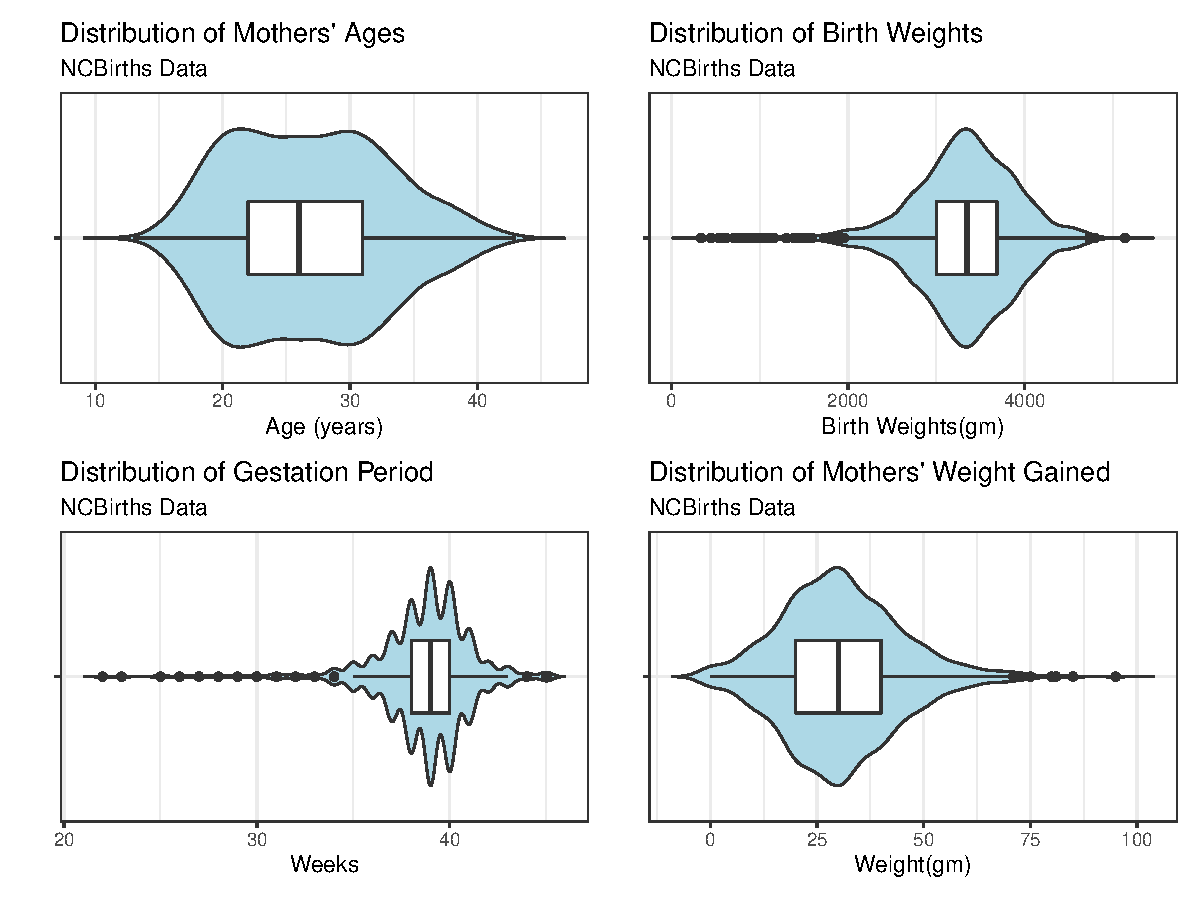
\includegraphics[width=\maxwidth]{figure/unnamed-chunk-3-1} 
\end{knitrout}
\caption{Violin plots of each variable.}
\label{ViolinSummary}
\end{figure}

From \ref{ViolinSummary} there is noticeable variability in all of the quantitative variables. We also noticed that the plots for Birthweights and Gestation Period showed many outliers on the lower tail, indicating low birth weights. 

We also wanted to visualize the distributions of these variables.

\begin{knitrout}
\definecolor{shadecolor}{rgb}{0.969, 0.969, 0.969}\color{fgcolor}\begin{kframe}
\begin{alltt}
\hlstd{histogram.BirthWeight}\hlkwb{<-} \hlkwd{ggplot}\hlstd{(births,} \hlkwd{aes}\hlstd{(}\hlkwc{x}\hlstd{=BirthWeightGm))}\hlopt{+}
  \hlkwd{geom_histogram}\hlstd{(}\hlkwc{fill} \hlstd{=} \hlstr{"lightblue"}\hlstd{,}
                 \hlkwc{color} \hlstd{=} \hlstr{"black"}\hlstd{,}
                 \hlkwc{bins} \hlstd{=} \hlnum{5}\hlstd{)} \hlopt{+}
  \hlkwd{theme_bw}\hlstd{()} \hlopt{+}
  \hlkwd{xlab}\hlstd{(}\hlstr{"Birth Weights"}\hlstd{)}\hlopt{+}
  \hlkwd{ylab}\hlstd{(}\hlstr{"Count of Weight(gm)"}\hlstd{)}\hlopt{+}
  \hlkwd{ggtitle}\hlstd{(}\hlstr{"Frequencies of Birth Weights"}\hlstd{)}


\hlstd{histogram.Gestation}\hlkwb{<-} \hlkwd{ggplot}\hlstd{(births,} \hlkwd{aes}\hlstd{(}\hlkwc{x}\hlstd{=Weeks))}\hlopt{+}
  \hlkwd{geom_histogram}\hlstd{(}\hlkwc{fill} \hlstd{=} \hlstr{"lightblue"}\hlstd{,}
                 \hlkwc{color} \hlstd{=} \hlstr{"black"}\hlstd{,}
                 \hlkwc{bins} \hlstd{=} \hlnum{5}\hlstd{)} \hlopt{+}
  \hlkwd{theme_bw}\hlstd{()} \hlopt{+}
  \hlkwd{xlab}\hlstd{(}\hlstr{"Gestation Period"}\hlstd{)}\hlopt{+}
  \hlkwd{ylab}\hlstd{(}\hlstr{"Count of Weeks"}\hlstd{)}\hlopt{+}
  \hlkwd{ggtitle}\hlstd{(}\hlstr{"Frequencies of Gestation Periods"}\hlstd{)}

\hlstd{histogram.MomAge} \hlkwb{<-} \hlkwd{ggplot}\hlstd{(births,} \hlkwd{aes}\hlstd{(}\hlkwc{x}\hlstd{=MomAge))}\hlopt{+}
  \hlkwd{geom_histogram}\hlstd{(}\hlkwc{fill} \hlstd{=} \hlstr{"lightblue"}\hlstd{,}
                 \hlkwc{color} \hlstd{=} \hlstr{"black"}\hlstd{,}
                 \hlkwc{bins} \hlstd{=} \hlnum{5}\hlstd{)} \hlopt{+}
  \hlkwd{theme_bw}\hlstd{()} \hlopt{+}
  \hlkwd{xlab}\hlstd{(}\hlstr{"Ages of Mothers(years)"}\hlstd{)}\hlopt{+}
  \hlkwd{ylab}\hlstd{(}\hlstr{"Count of Ages"}\hlstd{)}\hlopt{+}
  \hlkwd{ggtitle}\hlstd{(}\hlstr{"Frequencies of Ages"}\hlstd{)}

\hlstd{histogram.Gained}\hlkwb{<-} \hlkwd{ggplot}\hlstd{(births,} \hlkwd{aes}\hlstd{(}\hlkwc{x}\hlstd{=Gained))}\hlopt{+}
  \hlkwd{geom_histogram}\hlstd{(}\hlkwc{fill} \hlstd{=} \hlstr{"lightblue"}\hlstd{,}
                 \hlkwc{color} \hlstd{=} \hlstr{"black"}\hlstd{,}
                 \hlkwc{bins} \hlstd{=} \hlnum{5}\hlstd{)} \hlopt{+}
  \hlkwd{theme_bw}\hlstd{()} \hlopt{+}
  \hlkwd{xlab}\hlstd{(}\hlstr{"Weight Gained"}\hlstd{)}\hlopt{+}
  \hlkwd{ylab}\hlstd{(}\hlstr{"Count of Weight(gm) Gained"}\hlstd{)}\hlopt{+}
  \hlkwd{ggtitle}\hlstd{(}\hlstr{"Frequencies of Gained Weights"}\hlstd{)}

\hlstd{histogram.BirthWeight} \hlopt{+} \hlstd{histogram.Gestation} \hlopt{+} \hlstd{histogram.MomAge} \hlopt{+} \hlstd{histogram.Gained}
\end{alltt}
\end{kframe}
\end{knitrout}

\begin{figure}[H]
\centering
\begin{knitrout}
\definecolor{shadecolor}{rgb}{0.969, 0.969, 0.969}\color{fgcolor}
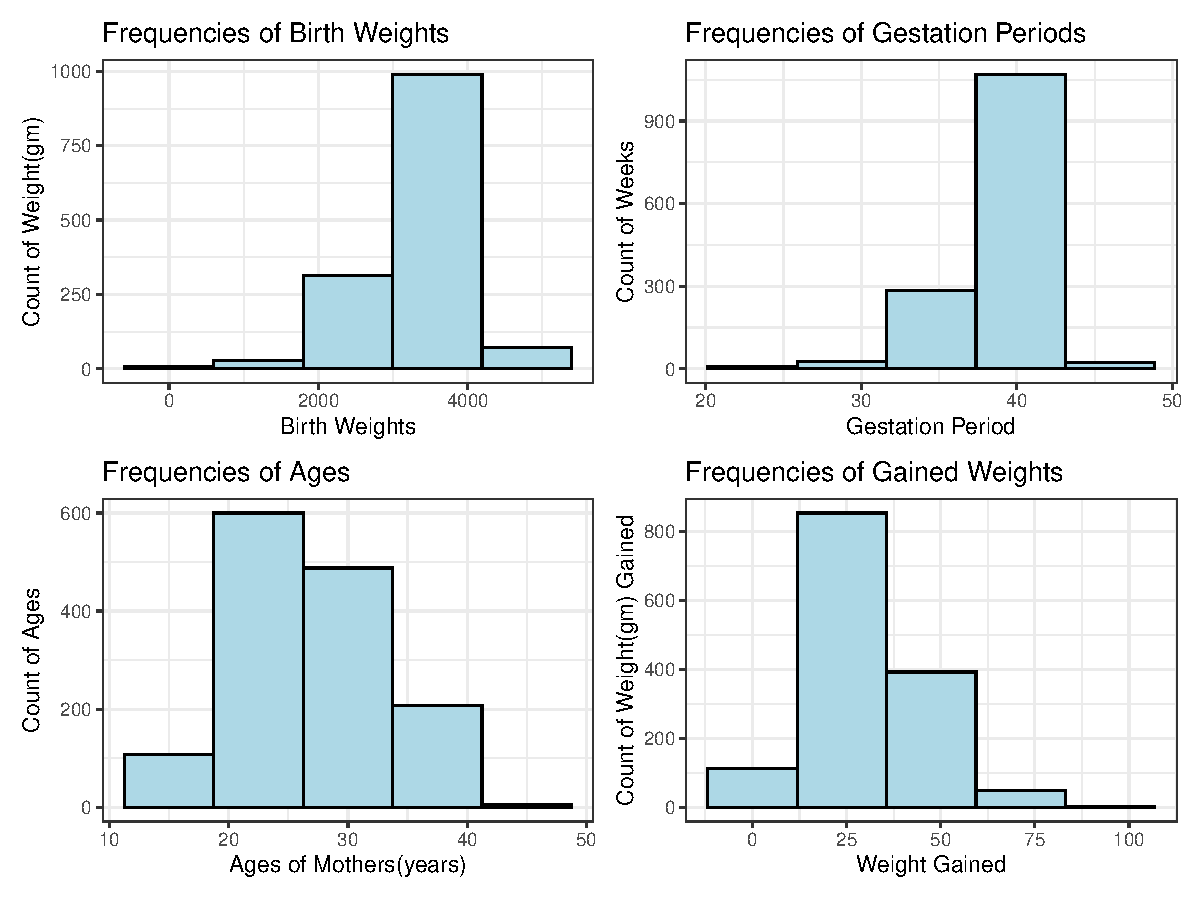
\includegraphics[width=\maxwidth]{figure/unnamed-chunk-4-1} 
\end{knitrout}
\caption{Grid of histograms for the quantitative variables.}
\label{HistogramSummary}
\end{figure}

\ref{HistogramSummary} shows that the quantitative variables do not follow normal distributions and are all skewed. We expected the distribution for birth weights and weeks of gestation to be similar in shape because those two variables are commonly known to be correlated. Typically babies that are born prematurely have low birth weights. 

We did find it interesting though, that the premature weights in the dataset influence the distribution more than we expected. 

We weren't sure if the preemie weights in the data set were outlier instances that were heavily skewing the distribution, or if there were just more preemies that we expected. To further investigate this, we created a bootstrap confidence interval to see whether the instances of low birth weights affected the lower end of our confidence interval for median birth weights. 

\begin{knitrout}
\definecolor{shadecolor}{rgb}{0.969, 0.969, 0.969}\color{fgcolor}\begin{kframe}
\begin{alltt}
\hlcom{## Bootstrapping for median weights }
\hlkwd{median}\hlstd{(births}\hlopt{$}\hlstd{BirthWeightGm)}
\end{alltt}
\begin{verbatim}
## [1] 3345.3
\end{verbatim}
\begin{alltt}
\hlkwd{set.seed}\hlstd{(}\hlnum{23}\hlstd{)}
\hlstd{alpha} \hlkwb{<-} \hlnum{0.05}
\hlstd{n} \hlkwb{<-} \hlkwd{nrow}\hlstd{(births)}
\hlstd{R} \hlkwb{<-} \hlnum{10000}
\hlstd{boot.stats} \hlkwb{<-} \hlkwd{rep}\hlstd{(}\hlnum{NA}\hlstd{, R)}
\hlkwa{for} \hlstd{(i} \hlkwa{in} \hlnum{1}\hlopt{:}\hlstd{R)\{}
  \hlstd{boot.data} \hlkwb{<-} \hlkwd{sample}\hlstd{(}\hlkwc{x} \hlstd{= births}\hlopt{$}\hlstd{BirthWeightGm,} \hlkwc{size} \hlstd{= n,} \hlkwc{replace} \hlstd{=} \hlnum{TRUE}\hlstd{)}
  \hlstd{boot.stats[i]} \hlkwb{<-} \hlkwd{median}\hlstd{(boot.data)}
\hlstd{\}}

\hlkwd{quantile}\hlstd{(boot.stats,} \hlkwc{probs} \hlstd{=} \hlkwd{c}\hlstd{(alpha}\hlopt{/}\hlnum{2}\hlstd{,} \hlnum{1} \hlopt{-} \hlstd{alpha}\hlopt{/}\hlnum{2}\hlstd{))}
\end{alltt}
\begin{verbatim}
##    2.5%   97.5% 
## 3316.95 3373.65
\end{verbatim}
\begin{alltt}
\hlstd{samp.boot.med} \hlkwb{<-} \hlkwa{function}\hlstd{(}\hlkwc{data}\hlstd{,} \hlkwc{indicies}\hlstd{)\{}
  \hlkwd{median}\hlstd{(data[indicies])}
\hlstd{\}}

\hlstd{boot.medians} \hlkwb{<-} \hlkwd{boot}\hlstd{(}\hlkwc{data} \hlstd{= births}\hlopt{$}\hlstd{BirthWeightGm,} \hlkwc{statistic} \hlstd{= samp.boot.med,} \hlkwc{R} \hlstd{=} \hlnum{10000}\hlstd{)}
\hlkwd{boot.ci}\hlstd{(boot.medians,} \hlkwc{conf} \hlstd{=} \hlnum{0.95}\hlstd{)}
\end{alltt}


{\ttfamily\noindent\color{warningcolor}{\#\# Warning in boot.ci(boot.medians, conf = 0.95): bootstrap variances needed for studentized intervals}}\begin{verbatim}
## BOOTSTRAP CONFIDENCE INTERVAL CALCULATIONS
## Based on 10000 bootstrap replicates
## 
## CALL : 
## boot.ci(boot.out = boot.medians, conf = 0.95)
## 
## Intervals : 
## Level      Normal              Basic         
## 95%   (3314, 3381 )   (3317, 3374 )  
## 
## Level     Percentile            BCa          
## 95%   (3317, 3374 )   (3289, 3345 )  
## Calculations and Intervals on Original Scale
## Some BCa intervals may be unstable
\end{verbatim}
\end{kframe}
\end{knitrout}

The median birth weight, M, calculated from our dataset was 3,345.3 grams. Our CI = $(3316.95, 3373.65)$ contained our median birth weight, and the lower bound aligned with the World Health Organization's statistic of 3,300 grams. We determined that the premature instances were not as influential as we suspected, and we continued without additional changes to the dataset. 

\item\textbf{Numerically summarize the variables in your dataset.}
\begin{knitrout}
\definecolor{shadecolor}{rgb}{0.969, 0.969, 0.969}\color{fgcolor}\begin{kframe}
\begin{alltt}
\hlcom{#add in weeks }
\hlstd{(sumstats} \hlkwb{<-} \hlstd{births} \hlopt \hlkwd{summarize}\hlstd{(}\hlkwc{meanW}\hlstd{=}\hlkwd{mean}\hlstd{(BirthWeightGm),}
                                 \hlkwc{medianW} \hlstd{=} \hlkwd{median}\hlstd{(BirthWeightGm),}
                                  \hlkwc{varianceW}\hlstd{=}\hlkwd{var}\hlstd{(BirthWeightGm),}
                                 \hlkwc{meanA}\hlstd{=}\hlkwd{mean}\hlstd{(MomAge),}
                                 \hlkwc{medianA}\hlstd{=}\hlkwd{median}\hlstd{(MomAge),}
                                 \hlkwc{varianceA} \hlstd{=} \hlkwd{var}\hlstd{(MomAge),}
                                 \hlkwc{meanWeeks} \hlstd{=} \hlkwd{mean}\hlstd{(Weeks),}
                                 \hlkwc{medianWeeks} \hlstd{=} \hlkwd{median}\hlstd{(Weeks),}
                                 \hlkwc{varianceWeeks} \hlstd{=} \hlkwd{var}\hlstd{(Weeks),}
                                 \hlkwc{meanW}\hlstd{=}\hlkwd{mean}\hlstd{(Gained),}
                                 \hlkwc{medianW} \hlstd{=} \hlkwd{median}\hlstd{(Gained),}
                                \hlkwc{varianceW}\hlstd{=}\hlkwd{var}\hlstd{(Gained)))}
\end{alltt}
\begin{verbatim}
## # A tibble: 1 x 9
##   meanW medianW varianceW meanA medianA varianceA meanWeeks medianWeeks varian~1
##   <dbl>   <dbl>     <dbl> <dbl>   <dbl>     <dbl>     <dbl>       <dbl>    <dbl>
## 1  30.6      30      193.  26.8      26      37.1      38.6          39     7.04
## # ... with abbreviated variable name 1: varianceWeeks
\end{verbatim}
\begin{alltt}
\hlstd{(}\hlkwd{var}\hlstd{(births}\hlopt{$}\hlstd{Gained))}
\end{alltt}
\begin{verbatim}
## [1] 192.5305
\end{verbatim}
\begin{alltt}
\hlkwd{xtable}\hlstd{(sumstats)}
\end{alltt}
\begin{verbatim}
## % latex table generated in R 4.2.1 by xtable 1.8-4 package
## % Thu Dec  8 04:25:38 2022
## \begin{table}[ht]
## \centering
## \begin{tabular}{rrrrrrrrrr}
##   \hline
##  & meanW & medianW & varianceW & meanA & medianA & varianceA & meanWeeks & medianWeeks & varianceWeeks \\ 
##   \hline
## 1 & 30.59 & 30.00 & 192.53 & 26.79 & 26.00 & 37.08 & 38.65 & 39.00 & 7.04 \\ 
##    \hline
## \end{tabular}
## \end{table}
\end{verbatim}
\end{kframe}
\end{knitrout}

\begin{table}[H]
\centering
\begin{tabular}{lrrrr}
  \hline
  Variable & mean & median & variance \\ 
  \hline
  Birth weight & 30.59 & 30.00 & 192.53\\
  Mother's age & 26.79 & 26.00 & 37.08 \\
  Gestation(weeks) & 38.65 & 39.00 & 7.04 \\ 
  Weight gained & 30.58978 & 30 & 192.5305 \\
  \hline
\end{tabular}
\caption{Numeric Summary of our quantitative variables.}
\end{table}

One of our initial assumptions pertained to the race of the mother, so we wanted to visualize this categorical variable with preemie, another categorical variable. The bar chart below shows the percentage of race that corresponds to the number of premature and not premature babies. 

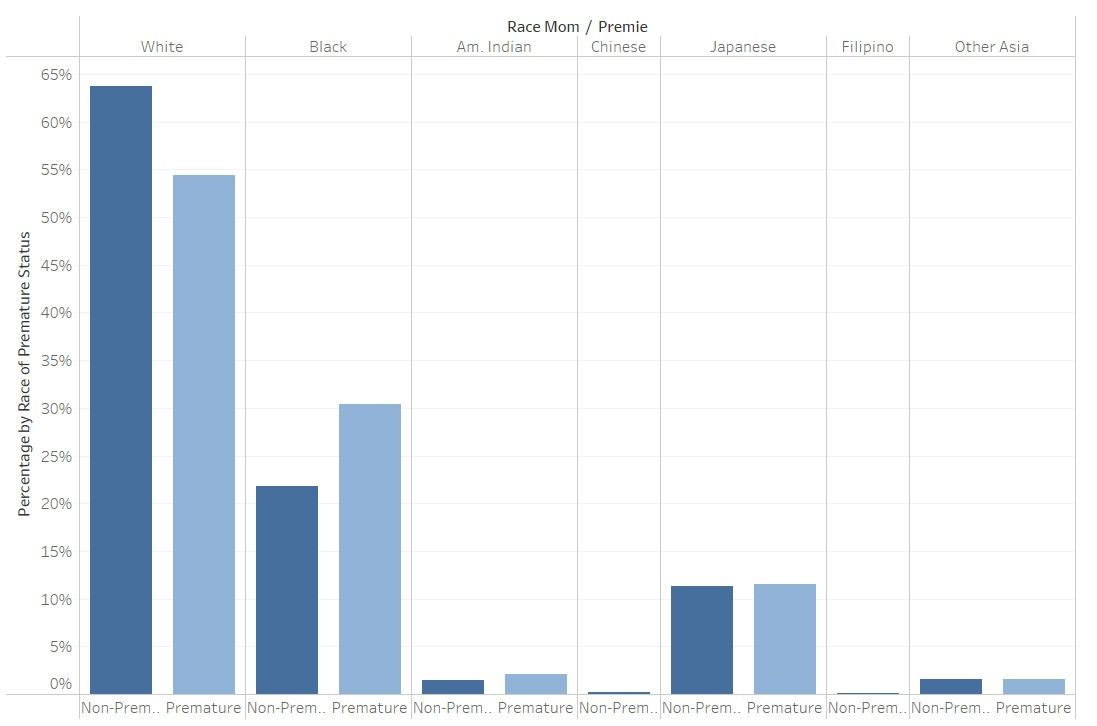
\includegraphics{./RacePremiePercent.jpg}

 We can see that white has the highest percentages for both preemies and non-preemies, however this does not necessarily mean that white is the most significant race predictor. There are 885 instances in which the mother of the child is white, which is more than half the dataset. So we focused on the race with a higher percentage of preemies compared to non-preemies, which was black. This observation aligns with our initial assumption that black should appear in our model. 

\item\textbf{Scatterplot Matrix and Table of Correlations}
\begin{knitrout}
\definecolor{shadecolor}{rgb}{0.969, 0.969, 0.969}\color{fgcolor}\begin{kframe}
\begin{alltt}
\hlstd{correlationsmatrix} \hlkwb{<-} \hlkwd{ggpairs}\hlstd{(births,} \hlkwc{columns} \hlstd{=} \hlkwd{c}\hlstd{(}\hlnum{4}\hlstd{,}\hlnum{5}\hlstd{,}\hlnum{9}\hlstd{,}\hlnum{12}\hlstd{))}
\hlstd{correlationsmatrix}
\end{alltt}
\end{kframe}
\end{knitrout}

\begin{figure}[H]
\centering
\begin{knitrout}
\definecolor{shadecolor}{rgb}{0.969, 0.969, 0.969}\color{fgcolor}
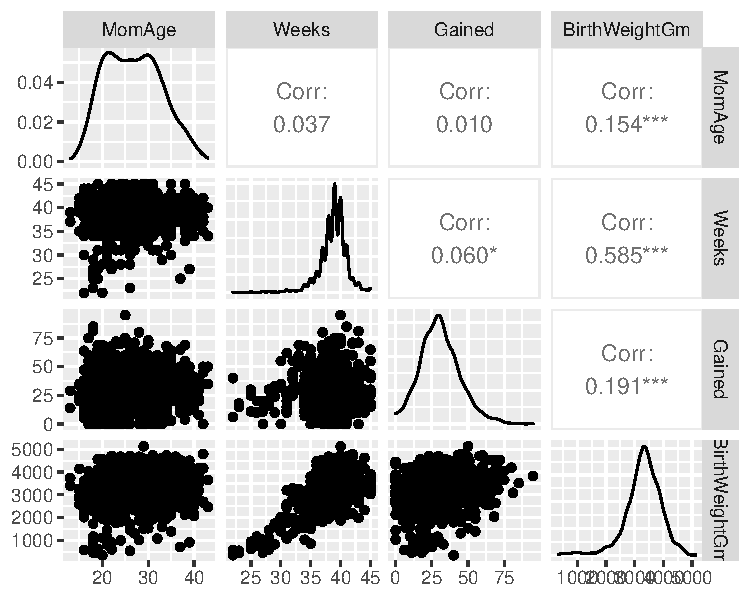
\includegraphics[width=\maxwidth]{figure/unnamed-chunk-7-1} 
\end{knitrout}
\caption{Matrix of ScatterPlots and Correlations for the variables.}
\label{CorrelationSummary}
\end{figure}

From \ref{CorrelationSummary} we can see that the relationship between birth weight and weeks coincides with our initial assumption, and they are correlated. However, we expected the correlation coefficient to be closer to 1 and it was only 0.585. Though the coefficients for the other variables in the matrix were positive, they were not high enough to be significant. Therefore, we could not make any assumptions about the model and which quantitative variables would be included at this point.

\end{enumerate}

Before we began with our first order model, we eliminated Low, a catagorical predictor that indicates true if the birth weight was low and false if the birth weight was not low. This attribute is originally calculated off of birth weight, which is our response variable. Excluding this predictor from the model eliminates any skew or strong false influence in our model from data that we could not know without having already had the response variable provided to us.

\section{First-Order Model and Model Selection.}

Before we began generating models, we first built several functions that would make analysis of the data more straightforward. One of these was to measure a statistic we devised and termed the "quantile departure" (QD) statistic. After scaling the residuals and sorting them in order, it measures how much the actual quantile positioning of each residual in a model departs from the theoretical quantiles of the model, calculated using q-norm. The value it returns is equivalent to: 

\begin{align*}
\frac{\sum_{i=1}^{n}|R_i - T_i|}{n}
\end{align*}

where $R_i$ is equal to the $i^{th}$ lowest actual residual and $T_i$ is the $i^{th}$ lowest theoretical residual. A higher value would indicate a higher departure from the theoretical quantiles, while a lower value would indicate residuals more consistent with the theoretical quantiles. 
\begin{knitrout}
\definecolor{shadecolor}{rgb}{0.969, 0.969, 0.969}\color{fgcolor}\begin{kframe}
\begin{alltt}
\hlcom{#create functions}
\hlcom{#Calculates the residuals departure from the theoretical quantiles, returning the mean abs() value of the actual minus theoretical quantiles }
\hlstd{quantDepart} \hlkwb{<-} \hlkwa{function}\hlstd{(}\hlkwc{model}\hlstd{) \{}
  \hlstd{residuals} \hlkwb{<-} \hlkwd{sort}\hlstd{(}\hlkwd{scale}\hlstd{(model}\hlopt{$}\hlstd{residuals,} \hlkwc{scale}\hlstd{=T))}
  \hlstd{i} \hlkwb{<-} \hlnum{1}\hlopt{:}\hlkwd{length}\hlstd{(residuals)}
  \hlstd{fi} \hlkwb{<-} \hlstd{(i} \hlopt{-} \hlnum{0.5}\hlstd{)} \hlopt{/} \hlkwd{length}\hlstd{(residuals)}
  \hlstd{x.norm} \hlkwb{<-} \hlkwd{qnorm}\hlstd{(fi)}

  \hlkwd{mean}\hlstd{(}\hlkwd{abs}\hlstd{(residuals} \hlopt{-} \hlstd{x.norm))}
\hlstd{\}}

\hlcom{#Displays a variety of summary stats and graphics of the model tailored based off of the specific options attributes set to True}
\hlstd{modelSummary} \hlkwb{<-} \hlkwa{function}\hlstd{(}\hlkwc{model}\hlstd{,} \hlkwc{coef}\hlstd{=T,} \hlkwc{stat}\hlstd{=T,} \hlkwc{plot}\hlstd{=T)\{}
  \hlkwa{if}\hlstd{(coef) \{}
    \hlkwd{print}\hlstd{(}\hlkwd{round}\hlstd{(}\hlkwd{summary}\hlstd{(model)}\hlopt{$}\hlstd{coefficients,}\hlnum{10}\hlstd{))}
  \hlstd{\}}
  \hlkwa{if}\hlstd{(stat) \{}
    \hlkwd{print}\hlstd{(}\hlkwd{paste}\hlstd{(}\hlstr{"R-squared:"}\hlstd{,} \hlkwd{summary}\hlstd{(model)}\hlopt{$}\hlstd{r.squared))}
    \hlkwd{print}\hlstd{(}\hlkwd{paste}\hlstd{(}\hlstr{"Adjusted R-Squared:"}\hlstd{,} \hlkwd{summary}\hlstd{(model)}\hlopt{$}\hlstd{adj.r.squared))}
    \hlkwd{print}\hlstd{(}\hlkwd{paste}\hlstd{(}\hlstr{"RMSE:"}\hlstd{,} \hlkwd{summary}\hlstd{(model)}\hlopt{$}\hlstd{sigma))}
    \hlkwd{print}\hlstd{(}\hlkwd{paste}\hlstd{(}\hlstr{"AIC:"}\hlstd{,} \hlkwd{AIC}\hlstd{(model)))}
    \hlkwd{print}\hlstd{(}\hlkwd{paste}\hlstd{(}\hlstr{"BIC:"}\hlstd{,} \hlkwd{BIC}\hlstd{(model)))}
    \hlkwd{print}\hlstd{(}\hlkwd{paste}\hlstd{(}\hlstr{"Quantile Departure:"}\hlstd{,} \hlkwd{quantDepart}\hlstd{(model)))}
  \hlstd{\}}
  \hlkwa{if}\hlstd{(plot) \{}
    \hlkwd{plotResiduals}\hlstd{(model)}
  \hlstd{\}}
\hlstd{\}}

\hlcom{#Calculates the  R squared of predicted vs actual values }
\hlstd{r_squared} \hlkwb{<-} \hlkwa{function}\hlstd{(}\hlkwc{actual}\hlstd{,} \hlkwc{predicted}\hlstd{) \{}
  \hlkwd{cor}\hlstd{(actual, predicted)}\hlopt{^}\hlnum{2}
\hlstd{\}}

\hlcom{#If provided with a model and a number of subsets of data, this will generate summary statistics for those subsets }
\hlstd{predictForSubsets} \hlkwb{<-} \hlkwa{function}\hlstd{(}\hlkwc{model}\hlstd{,} \hlkwc{class.attr}\hlstd{,} \hlkwc{...}\hlstd{,} \hlkwc{names}\hlstd{=}\hlkwd{c}\hlstd{()) \{}
  \hlstd{x} \hlkwb{<-} \hlkwd{list}\hlstd{(...)}
  \hlstd{i} \hlkwb{<-} \hlnum{1}
  \hlstd{residPlots} \hlkwb{<-} \hlkwd{list}\hlstd{()}
  \hlstd{predPlots} \hlkwb{<-} \hlkwd{list}\hlstd{()}
  \hlkwa{for} \hlstd{(v} \hlkwa{in} \hlstd{x) \{}
    \hlstd{v}\hlopt{$}\hlstd{predict} \hlkwb{<-} \hlkwd{predict}\hlstd{(model, v)}
    \hlstd{v}\hlopt{$}\hlstd{resid} \hlkwb{<-} \hlstd{v[[class.attr]]} \hlopt{-} \hlstd{v}\hlopt{$}\hlstd{predict}
    \hlstd{subsetName} \hlkwb{<-} \hlstr{""}
    \hlkwa{if} \hlstd{(}\hlkwd{length}\hlstd{(names)} \hlopt{>=} \hlstd{i) \{}
      \hlstd{subsetName} \hlkwb{<-} \hlstd{names[i]}
    \hlstd{\}} \hlkwa{else} \hlstd{\{}
      \hlstd{subsetName} \hlkwb{<-} \hlkwd{paste}\hlstd{(}\hlstr{"Subset"}\hlstd{, i)}
    \hlstd{\}}
    \hlkwd{print}\hlstd{(}\hlkwd{paste}\hlstd{(subsetName,} \hlstr{"R-Squared:"}\hlstd{,} \hlkwd{r_squared}\hlstd{(v}\hlopt{$}\hlstd{predict, v[[class.attr]])))}
    \hlkwd{print}\hlstd{(}\hlkwd{paste}\hlstd{(subsetName,} \hlstr{"Mean Abs. Error:"}\hlstd{,} \hlkwd{mean}\hlstd{(}\hlkwd{abs}\hlstd{(v}\hlopt{$}\hlstd{resid))))}

    \hlkwd{ggplot}\hlstd{(}\hlkwc{data}\hlstd{=v,} \hlkwd{aes}\hlstd{(}\hlkwc{x}\hlstd{=predict,} \hlkwc{y}\hlstd{=resid))} \hlopt{+}
      \hlkwd{geom_point}\hlstd{(}\hlkwc{size}\hlstd{=}\hlnum{1}\hlstd{,}
                 \hlkwc{shape}\hlstd{=}\hlnum{16}\hlstd{)}\hlopt{+}
      \hlkwd{theme_bw}\hlstd{()}\hlopt{+}
      \hlkwd{xlab}\hlstd{(}\hlstr{"Predicted"}\hlstd{)}\hlopt{+}
      \hlkwd{ylab}\hlstd{(}\hlstr{"Residuals"}\hlstd{)}\hlkwb{->} \hlstd{residuals}
    \hlkwd{ggplot}\hlstd{(}\hlkwc{data}\hlstd{=v,} \hlkwd{aes}\hlstd{(}\hlkwc{x}\hlstd{=predict,} \hlkwc{y}\hlstd{=}\hlkwd{get}\hlstd{(class.attr)))} \hlopt{+}
      \hlkwd{geom_point}\hlstd{(}\hlkwc{size}\hlstd{=}\hlnum{1}\hlstd{,}
                 \hlkwc{shape}\hlstd{=}\hlnum{16}\hlstd{)}\hlopt{+}
      \hlkwd{theme_bw}\hlstd{()}\hlopt{+}
      \hlkwd{xlab}\hlstd{(}\hlstr{"Predicted"}\hlstd{)}\hlopt{+}
      \hlkwd{ylab}\hlstd{(}\hlstr{"Actual"}\hlstd{)} \hlkwb{->} \hlstd{predictions}
    \hlkwa{if} \hlstd{(}\hlkwd{length}\hlstd{(x)} \hlopt{!=} \hlnum{3}\hlstd{) \{}
      \hlkwd{print}\hlstd{((predictions} \hlopt{+} \hlkwd{ggtitle}\hlstd{(}\hlstr{"Predicted versus Actual"}\hlstd{,}
           \hlkwc{subtitle}\hlstd{=subsetName))} \hlopt{+} \hlstd{(residuals} \hlopt{+} \hlkwd{ggtitle}\hlstd{(}\hlstr{"Predicted versus Residuals"}\hlstd{,}
           \hlkwc{subtitle}\hlstd{=subsetName)))}
    \hlstd{\}} \hlkwa{else} \hlstd{\{}
      \hlstd{residPlots} \hlkwb{<-} \hlkwd{append}\hlstd{(residPlots,} \hlkwd{list}\hlstd{(residuals} \hlopt{+} \hlkwd{ggtitle}\hlstd{(}\hlstr{""}\hlstd{,} \hlkwc{subtitle}\hlstd{=subsetName)))}
      \hlstd{predPlots} \hlkwb{<-} \hlkwd{append}\hlstd{(predPlots,} \hlkwd{list}\hlstd{(predictions} \hlopt{+} \hlkwd{ggtitle}\hlstd{(}\hlstr{""}\hlstd{,} \hlkwc{subtitle}\hlstd{=subsetName)))}
    \hlstd{\}}
    \hlstd{i} \hlkwb{<-} \hlstd{i} \hlopt{+} \hlnum{1}
  \hlstd{\}}
  \hlkwa{if} \hlstd{(}\hlkwd{length}\hlstd{(x)} \hlopt{==} \hlnum{3}\hlstd{) \{}
    \hlstd{topPatch} \hlkwb{<-} \hlstd{(residPlots[[}\hlnum{1}\hlstd{]]} \hlopt{+} \hlstd{residPlots[[}\hlnum{2}\hlstd{]]} \hlopt{+} \hlstd{residPlots[[}\hlnum{3}\hlstd{]])}
    \hlstd{bottomPatch} \hlkwb{<-} \hlstd{(predPlots[[}\hlnum{1}\hlstd{]]} \hlopt{+} \hlstd{predPlots[[}\hlnum{2}\hlstd{]]} \hlopt{+} \hlstd{predPlots[[}\hlnum{3}\hlstd{]])}
    \hlstd{combine} \hlkwb{<-} \hlkwd{wrap_elements}\hlstd{(topPatch} \hlopt{+} \hlkwd{plot_annotation}\hlstd{(}\hlkwc{title} \hlstd{=} \hlstr{"Predicted verses Residuals"}\hlstd{))} \hlopt{/}
                \hlkwd{wrap_elements}\hlstd{(bottomPatch} \hlopt{+} \hlkwd{plot_annotation}\hlstd{(}\hlkwc{title} \hlstd{=} \hlstr{"Predicted verses Actual"}\hlstd{))}
    \hlkwd{print}\hlstd{(combine)}
  \hlstd{\}}

\hlstd{\}}
\end{alltt}
\end{kframe}
\end{knitrout}

\subsection{First Order Model}
Before we began with our first order model, we eliminated Low, a catagorical predictor that indicates true if the birth weight was low and false if the birth weight was not low. This predictor was calculated off of BirthWeightGm, which is our response variable. Excluding this predictor from the model eliminates any skew or strong false influence in our model. 

Fitting a first-order linear model with all our acceptable predictor variables, we calculated the following estimated linear regression equation: \\

\begin{align*} \hat{y} &= -964.29 - 704.71\cdot \text{I}(\text{Plural} = 2) - 932.13\cdot \text{I}(\text{Plural} = 3) + 93.90\cdot \text{I}(\text{Sex} = \text{Male}) \\ &\quad + 10.88\cdot \text{MomAge} + 97.81\cdot \text{Weeks} -76.88\cdot \text{I}(\text{RaceMom} = \text{Black}) + 81.31\cdot \text{I}(\text{RaceMom} = \text{Chinese}) \\ &\quad -860.40\cdot \text{I}(\text{RaceMom} = \text{Filipino}) + 29.04\cdot \text{I}(\text{RaceMom} = \text{Japanese}) -58.43\cdot \text{I}(\text{RaceMom} = \text{Other\ Asian/PI}) \\ &\quad + 30.78\cdot \text{I}(\text{RaceMom} = \text{White}) -48.07\cdot \text{I}(\text{Marital} = \text{Unmarried}) + 7.87\cdot \text{Gained} \\ &\quad -203.49\cdot \text{I}(\text{Smoke} = \text{Yes}) -217.62\cdot \text{I}(\text{Preemie} = \text{Yes}) \end{align*}

  
\begin{knitrout}
\definecolor{shadecolor}{rgb}{0.969, 0.969, 0.969}\color{fgcolor}\begin{kframe}
\begin{alltt}
\hlcom{#first model = model.1}
\hlkwd{lm}\hlstd{(BirthWeightGm} \hlopt{~} \hlstd{Plural} \hlopt{+} \hlstd{Sex} \hlopt{+} \hlstd{MomAge} \hlopt{+} \hlstd{Weeks} \hlopt{+} \hlstd{RaceMom} \hlopt{+}
     \hlstd{Marital} \hlopt{+} \hlstd{Gained} \hlopt{+} \hlstd{Smoke} \hlopt{+} \hlstd{Preemie, births)} \hlkwb{->} \hlstd{model.1}

\hlkwd{modelSummary}\hlstd{(model.1,} \hlkwc{plot}\hlstd{=}\hlnum{FALSE}\hlstd{)}
\end{alltt}
\begin{verbatim}
##                           Estimate  Std. Error    t value     Pr(>|t|)
## (Intercept)             -964.28919 294.9607224 -3.2692122 0.0011048007
## Plural2                 -704.70670  76.5727750 -9.2030973 0.0000000000
## Plural3                 -932.12784 237.3884857 -3.9265925 0.0000903705
## SexMale                   93.89649  24.8249532  3.7823432 0.0001619382
## MomAge                    10.88077   2.3232147  4.6834980 0.0000030955
## Weeks                     97.81144   6.8023799 14.3790033 0.0000000000
## RaceMomBlack             -76.87702 102.7336877 -0.7483137 0.4543973043
## RaceMomChinese            81.30745 344.1690322  0.2362428 0.8132790072
## RaceMomFilipino         -860.40322 476.1359772 -1.8070536 0.0709696081
## RaceMomJapanese           29.03632 106.7611068  0.2719747 0.7856817781
## RaceMomOther Asian / PI  -58.43107 140.9347082 -0.4145967 0.6785009952
## RaceMomWhite              30.78400 101.2713293  0.3039755 0.7611919583
## MaritalUnmarried         -48.07301  32.1293957 -1.4962315 0.1348198655
## Gained                     7.86655   0.9098714  8.6457814 0.0000000000
## SmokeYes                -203.48734  36.5920140 -5.5609767 0.0000000321
## PreemieYes              -217.62136  53.3527133 -4.0789183 0.0000478089
## [1] "R-squared: 0.45706523101896"
## [1] "Adjusted R-Squared: 0.451218840828927"
## [1] "RMSE: 464.671921644458"
## [1] "AIC: 21322.7497301962"
## [1] "BIC: 21412.0105338985"
## [1] "Quantile Departure: 0.0472456539674342"
\end{verbatim}
\end{kframe}
\end{knitrout}
  
\begin{knitrout}
\definecolor{shadecolor}{rgb}{0.969, 0.969, 0.969}\color{fgcolor}\begin{kframe}
\begin{alltt}
\hlkwd{xtable}\hlstd{(model.1,} \hlkwc{caption}\hlstd{=}\hlstr{"Predictor Statistics and Significance for First-Order Model"}\hlstd{,} \hlkwc{label}\hlstd{=}\hlstr{"First.Order.Table"}\hlstd{)}
\end{alltt}
\end{kframe}
\end{knitrout}

\begin{table}[H]
\centering
\begin{tabular}{lrrrrrr}
  \hline
$R^2$ & $R^2_{adj}$ & RSE & AIC & BIC & RD\\ 
  \hline
   0.4570 & 0.4512 & 464.6719 & 21322.7497 & 21412.0105 & 0.0472 \\ 
   \hline
\end{tabular}
\caption{Summary of first order regression model R-squared, Adj R-squared, RSE, AIC, and BIC.}
\label{first.order.summary}
\end{table}

As Table \ref{First.Order.Table} indicates, Plural2 (Twins), Plural3 (Triplets), Sex = Male, MomAge, Weeks, RaceMom = Filipino, Gained, Smoke, and Preemie are all significant predictors. Table \ref{first.order.summary} demonstrates that the $R^2$ is fairly high, meaning the model is quite predictive; additionally, the quantile departure value is very close to 0, meaning it does well to satisfy the requirements for equal distribution of residuals. This is further emphasized in Figure \ref{resid.plots.un}. However, AIC and BIC values are also high, meaning that the number of predictor variables is not predictive enough to justify the variety of parameters we are using.

\begin{knitrout}
\definecolor{shadecolor}{rgb}{0.969, 0.969, 0.969}\color{fgcolor}\begin{kframe}
\begin{alltt}
\hlcom{# Log of Weight}
\hlkwd{lm}\hlstd{(WeightGmLog} \hlopt{~} \hlstd{Plural} \hlopt{+} \hlstd{Sex} \hlopt{+} \hlstd{MomAgeSC} \hlopt{+} \hlstd{WeeksSC} \hlopt{+} \hlstd{RaceMom} \hlopt{+}
     \hlstd{Marital} \hlopt{+} \hlstd{GainedSC} \hlopt{+} \hlstd{Smoke} \hlopt{+} \hlstd{Preemie, births)} \hlkwb{->} \hlstd{model.log}

\hlcom{# Square Root of Weight}
\hlkwd{lm}\hlstd{(WeightGmSqrt} \hlopt{~} \hlstd{Plural} \hlopt{+} \hlstd{Sex} \hlopt{+} \hlstd{MomAgeSC} \hlopt{+} \hlstd{WeeksSC} \hlopt{+} \hlstd{RaceMom} \hlopt{+}
     \hlstd{Marital} \hlopt{+} \hlstd{GainedSC} \hlopt{+} \hlstd{Smoke} \hlopt{+} \hlstd{Preemie, births)} \hlkwb{->} \hlstd{model.sqrt}

\hlcom{# Squared of Weight}
\hlkwd{lm}\hlstd{(WeightGmS} \hlopt{~} \hlstd{Plural} \hlopt{+} \hlstd{Sex} \hlopt{+} \hlstd{MomAgeSC} \hlopt{+} \hlstd{WeeksSC} \hlopt{+} \hlstd{RaceMom} \hlopt{+}
     \hlstd{Marital} \hlopt{+} \hlstd{GainedSC} \hlopt{+} \hlstd{Smoke} \hlopt{+} \hlstd{Preemie, births)} \hlkwb{->} \hlstd{model.s}

\hlcom{# Square of the Log of Weight}
\hlkwd{lm}\hlstd{(WeightGmSLog} \hlopt{~} \hlstd{Plural} \hlopt{+} \hlstd{Sex} \hlopt{+} \hlstd{MomAgeSC} \hlopt{+} \hlstd{WeeksSC} \hlopt{+} \hlstd{RaceMom} \hlopt{+}
     \hlstd{Marital} \hlopt{+} \hlstd{GainedSC} \hlopt{+} \hlstd{Smoke} \hlopt{+} \hlstd{Preemie, births)} \hlkwb{->} \hlstd{model.slog}

\hlcom{# Log of the Log of Weight}
\hlkwd{lm}\hlstd{(WeightGmLogLog} \hlopt{~} \hlstd{Plural} \hlopt{+} \hlstd{Sex} \hlopt{+} \hlstd{MomAgeSC} \hlopt{+} \hlstd{WeeksSC} \hlopt{+} \hlstd{RaceMom} \hlopt{+}
     \hlstd{Marital} \hlopt{+} \hlstd{GainedSC} \hlopt{+} \hlstd{Smoke} \hlopt{+} \hlstd{Preemie, births)} \hlkwb{->} \hlstd{model.loglog}

\hlcom{# Log of the Square Root of Weight}
\hlkwd{lm}\hlstd{(WeightGmLogSqr} \hlopt{~} \hlstd{Plural} \hlopt{+} \hlstd{Sex} \hlopt{+} \hlstd{MomAgeSC} \hlopt{+} \hlstd{WeeksSC} \hlopt{+} \hlstd{RaceMom} \hlopt{+}
     \hlstd{Marital} \hlopt{+} \hlstd{GainedSC} \hlopt{+} \hlstd{Smoke} \hlopt{+} \hlstd{Preemie, births)} \hlkwb{->} \hlstd{model.logsqr}

\hlcom{# Square Root of the Log of Weight}
\hlkwd{lm}\hlstd{(WeightGmSqrtLog} \hlopt{~} \hlstd{Plural} \hlopt{+} \hlstd{Sex} \hlopt{+} \hlstd{MomAgeSC} \hlopt{+} \hlstd{WeeksSC} \hlopt{+} \hlstd{RaceMom} \hlopt{+}
     \hlstd{Marital} \hlopt{+} \hlstd{GainedSC} \hlopt{+} \hlstd{Smoke} \hlopt{+} \hlstd{Preemie, births)} \hlkwb{->} \hlstd{model.sqrtlog}

\hlcom{# Inverse of the Weight}
\hlkwd{lm}\hlstd{(WeightGmInverse} \hlopt{~} \hlstd{Plural} \hlopt{+} \hlstd{Sex} \hlopt{+} \hlstd{MomAgeSC} \hlopt{+} \hlstd{WeeksSC} \hlopt{+} \hlstd{RaceMom} \hlopt{+}
     \hlstd{Marital} \hlopt{+} \hlstd{GainedSC} \hlopt{+} \hlstd{Smoke} \hlopt{+} \hlstd{Preemie, births)} \hlkwb{->} \hlstd{model.inverse}
\end{alltt}
\end{kframe}
\end{knitrout}

Before eliminating the non-significant variables from our model we wanted to test transformations of BirthWeight, to see if any of them improved our model performance statistics or residual distributions. The model statistics for each transformation are listed in Table \ref{tab.com.transform}. 

\begin{table}[H]
\centering
\begin{tabular}{lrrrrrr}
  \hline
  Transformation & $R^2$ & $R^2_{adj}$ & RSE & AIC & BIC & QD\\ 
  \hline
   No Transformation & 0.4570 & 0.4512 & 464.7 & 21322 & 21412 & 0.0472 \\ 
   $log$ of Weight & 0.5243 & 0.5192 & 0.1756 & -885.3 & -796 & 0.1573\\ 
   Square Root of Weight & 0.4994 & 0.4940 & 4.3160 & 8137 & 8227 & 0.0787 \\
   Weight Squared & 0.3699 & 0.3631 & $3.04 * 10^6$ & 46086 & 46175 & 0.0974 \\
   $log$ of Weight Squared & 0.5208 & 0.5156 & 2.7 & 6812 & 6901 & 0.1340\\
   $log$ of the $log$ of Weight & 0.5249 & 0.5198 & 0.0231 & -6597 & -6508 & 0.1824 \\
   $log$ of the Square Root of Weight & 0.5243 & 0.5192 & 0.3512 & 1068 & 1157 & 0.1573\\
   Square Root of the $log$ of Weight & 0.5250 & 0.5199 & 0.0318 & -5699 & -5610 & 0.1695\\
   Inverse of the Weight & 0.4507 & 0.4447 & 0.0001 & -21462 & -21373 & 0.3578 \\
   \hline
\end{tabular}
\caption{Summary of all adjusted first order regression model R-squared, Adj R-squared, RSE, AIC, and BIC.}
\label{tab.comp.transform}
\end{table}



Based on Table \ref{tab.comp.transform}, we have several potential transformation options. First is the un-transformed weight, which better satisfies the assumptions behind linear regression modeling, namely the equal
distribution of residuals. On the other hand, we have the log weight model, which has higher $R^2$ values and lower RMSE, AIC, and BIC values than most other models, meaning it is more accurate. This accuracy is, however, gained only at the expense of making residuals less equally distributed. As shown by the QD values, and emphasized by the comparisons between Figure \ref{resid.plots.un} and \ref{resid.plots.log}, the $log$ transformation results in a quantile departure nearly four times the size of the non-transformed. The residual disparities also seem to come much more from the lower end of the birth weights in the logarithmic model. Because of this, it does not seem to as strongly satisfy the assumptions necessary to do things like conduct statistical inference on parameters. Thus, we will be proceeding with two models, the assumptions model and the accuracy model, where one will seek to minimize departure from assumptions and the other will seek to maximize accuracy. Assumption models will use the scaled and centered gram weight as their target, while accuracy models will use the scaled and centered $log$ of gram weight.\\

Below are our two first-order models, one with no transformations and the other with the $log$ of the weight taken. Both have all numeric variables, including the response variables, scaled and centered.

\begin{knitrout}
\definecolor{shadecolor}{rgb}{0.969, 0.969, 0.969}\color{fgcolor}\begin{kframe}
\begin{alltt}
\hlcom{#First-Order Model with All Appropriate Transformations, and Numeric Attributes Scaled & Centered}
\hlkwd{lm}\hlstd{(WeightGmSC} \hlopt{~} \hlstd{Plural} \hlopt{+} \hlstd{Sex} \hlopt{+} \hlstd{MomAgeSC} \hlopt{+} \hlstd{WeeksSC} \hlopt{+} \hlstd{RaceMom} \hlopt{+}
     \hlstd{Marital} \hlopt{+} \hlstd{GainedSC} \hlopt{+} \hlstd{Smoke} \hlopt{+} \hlstd{Preemie, births)} \hlkwb{->} \hlstd{model.2.assu}

\hlkwd{modelSummary}\hlstd{(model.2.assu,} \hlkwc{coef}\hlstd{=F,} \hlkwc{stat}\hlstd{=F)}
\end{alltt}
\end{kframe}
\end{knitrout}

\begin{knitrout}
\definecolor{shadecolor}{rgb}{0.969, 0.969, 0.969}\color{fgcolor}\begin{kframe}
\begin{alltt}
\hlkwd{lm}\hlstd{(WeightLogSC} \hlopt{~} \hlstd{Plural} \hlopt{+} \hlstd{Sex} \hlopt{+} \hlstd{MomAgeSC} \hlopt{+} \hlstd{WeeksSC} \hlopt{+} \hlstd{RaceMom} \hlopt{+}
     \hlstd{Marital} \hlopt{+} \hlstd{GainedSC} \hlopt{+} \hlstd{Smoke} \hlopt{+} \hlstd{Preemie, births)} \hlkwb{->} \hlstd{model.2.accur}

\hlkwd{modelSummary}\hlstd{(model.2.accur,} \hlkwc{coef}\hlstd{=F,} \hlkwc{stat}\hlstd{=F)}
\end{alltt}
\end{kframe}
\end{knitrout}

\begin{figure}
\begin{knitrout}
\definecolor{shadecolor}{rgb}{0.969, 0.969, 0.969}\color{fgcolor}\begin{kframe}
\begin{alltt}
\hlcom{#First-Order Model with All Appropriate Transformations, and Numeric Attributes Scaled & Centered}
\hlkwd{lm}\hlstd{(WeightGmSC} \hlopt{~} \hlstd{Plural} \hlopt{+} \hlstd{Sex} \hlopt{+} \hlstd{MomAgeSC} \hlopt{+} \hlstd{WeeksSC} \hlopt{+} \hlstd{RaceMom} \hlopt{+}
     \hlstd{Marital} \hlopt{+} \hlstd{GainedSC} \hlopt{+} \hlstd{Smoke} \hlopt{+} \hlstd{Preemie, births)} \hlkwb{->} \hlstd{model.2.assu}

\hlkwd{modelSummary}\hlstd{(model.2.assu,} \hlkwc{coef}\hlstd{=F,} \hlkwc{stat}\hlstd{=F)}
\end{alltt}
\end{kframe}
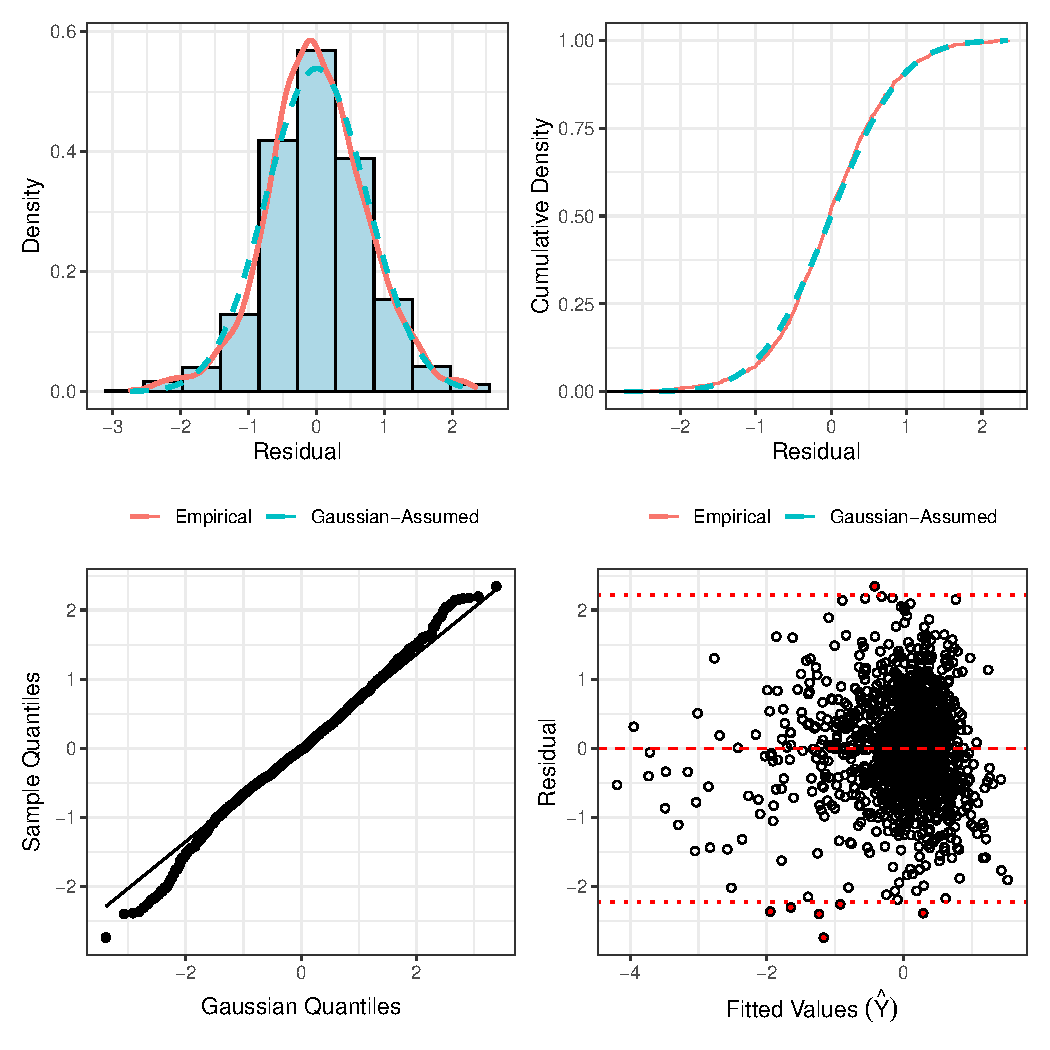
\includegraphics[width=\maxwidth]{figure/unnamed-chunk-12-1} 
\end{knitrout}
\caption{Residual Plots of Untransformed Model.} 
\label{resid.plots.un}
\end{figure}

\begin{figure}
\begin{knitrout}
\definecolor{shadecolor}{rgb}{0.969, 0.969, 0.969}\color{fgcolor}\begin{kframe}
\begin{alltt}
\hlkwd{lm}\hlstd{(WeightLogSC} \hlopt{~} \hlstd{Plural} \hlopt{+} \hlstd{Sex} \hlopt{+} \hlstd{MomAgeSC} \hlopt{+} \hlstd{WeeksSC} \hlopt{+} \hlstd{RaceMom} \hlopt{+}
     \hlstd{Marital} \hlopt{+} \hlstd{GainedSC} \hlopt{+} \hlstd{Smoke} \hlopt{+} \hlstd{Preemie, births)} \hlkwb{->} \hlstd{model.2.accur}

\hlkwd{modelSummary}\hlstd{(model.2.accur,} \hlkwc{coef}\hlstd{=F,} \hlkwc{stat}\hlstd{=F)}
\end{alltt}
\end{kframe}
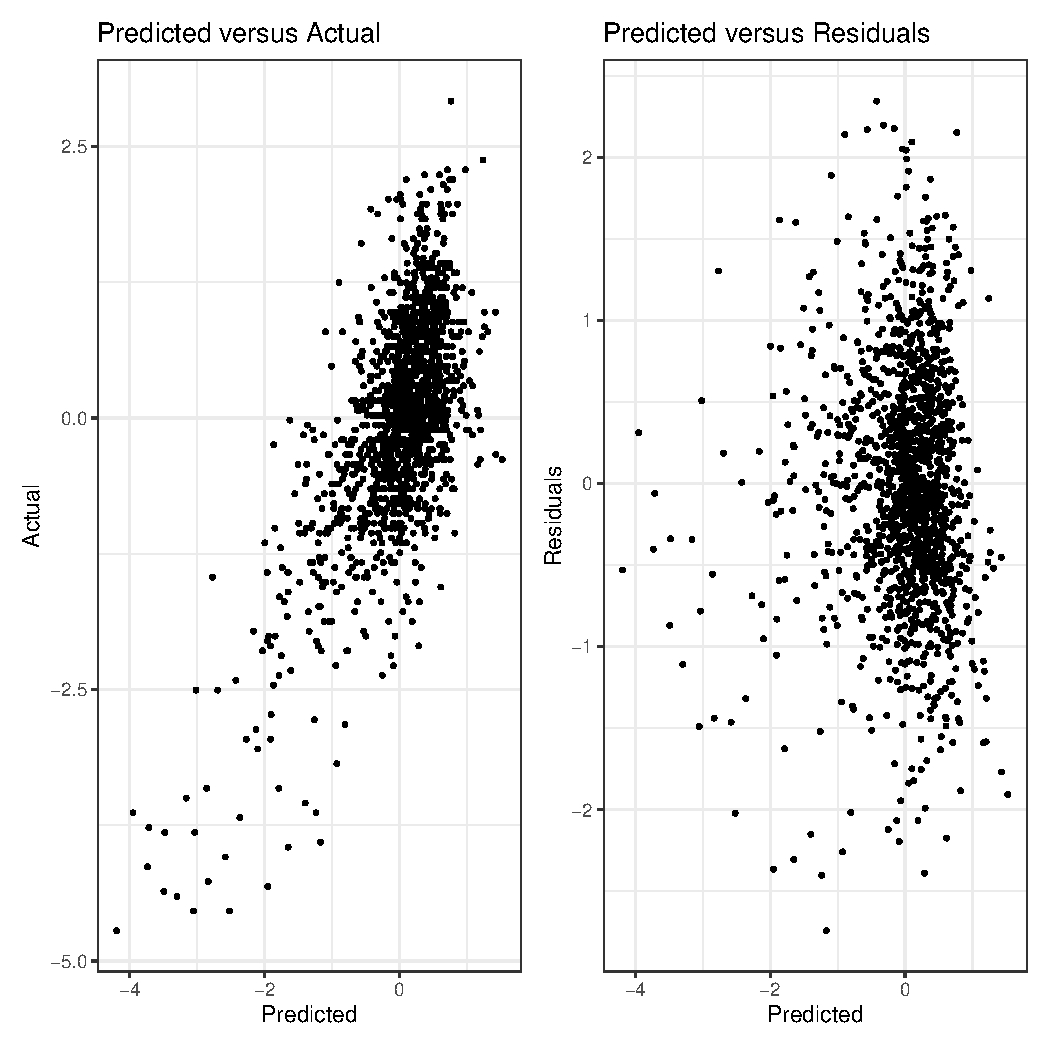
\includegraphics[width=\maxwidth]{figure/unnamed-chunk-13-1} 
\end{knitrout}
\caption{Residual Plots of Logarithmic Model.} 
\label{resid.plots.log}
\end{figure}

\subsection{First Order Model Pruning}\label{fom.prune}

Our next step was to reduce the number of variables in the two models to only those that had an affect. For both of our models, we ran AIC-based elimination, BIC-based elimination, and regression subset optimization techniques to determine which variables should be removed.

\begin{knitrout}
\definecolor{shadecolor}{rgb}{0.969, 0.969, 0.969}\color{fgcolor}\begin{kframe}
\begin{alltt}
\hlstd{x} \hlkwb{<-} \hlkwd{model.matrix}\hlstd{(model.2.assu)[,}\hlopt{-}\hlnum{1}\hlstd{]}

\hlstd{y} \hlkwb{<-} \hlstd{births}\hlopt{$}\hlstd{WeightGmSC}

\hlstd{xy} \hlkwb{<-} \hlkwd{as.data.frame}\hlstd{(}\hlkwd{cbind}\hlstd{(x,y))}
\hlstd{best.subsets.aic} \hlkwb{<-} \hlkwd{bestglm}\hlstd{(xy,} \hlkwc{IC}\hlstd{=}\hlstr{"AIC"}\hlstd{,} \hlkwc{TopModels} \hlstd{=} \hlnum{5}\hlstd{)}
\hlstd{best.model.aic} \hlkwb{<-} \hlstd{best.subsets.aic}\hlopt{$}\hlstd{BestModel}
\hlkwd{modelSummary}\hlstd{(best.model.aic,} \hlkwc{plot}\hlstd{=F)}
\end{alltt}
\begin{verbatim}
##                    Estimate Std. Error   t value     Pr(>|t|)
## (Intercept)       0.1155533 0.03565298  3.241056 0.0012189440
## Plural2          -1.1195941 0.12177905 -9.193651 0.0000000000
## Plural3          -1.4808912 0.37795193 -3.918200 0.0000935265
## SexMale           0.1502685 0.03951570  3.802753 0.0001492650
## MomAgeSC          0.1054359 0.02244925  4.696635 0.0000029051
## WeeksSC           0.4196465 0.02914455 14.398801 0.0000000000
## RaceMomBlack     -0.1665708 0.05073699 -3.283025 0.0010523894
## RaceMomFilipino  -1.4157231 0.74133018 -1.909706 0.0563756484
## MaritalUnmarried -0.0790069 0.05003876 -1.578914 0.1145821349
## GainedSC          0.1737710 0.01995059  8.710069 0.0000000000
## SmokeYes         -0.3216242 0.05699092 -5.643428 0.0000000202
## PreemieYes       -0.3511604 0.08474998 -4.143486 0.0000362603
## [1] "R-squared: 0.456717769215429"
## [1] "Adjusted R-Squared: 0.452439956374606"
## [1] "RMSE: 0.739973001957095"
## [1] "AIC: 3163.90042969188"
## [1] "BIC: 3232.15869134656"
## [1] "Quantile Departure: 0.0474199906966593"
\end{verbatim}
\begin{alltt}
\hlstd{best.subsets.bic} \hlkwb{<-} \hlkwd{bestglm}\hlstd{(xy,} \hlkwc{IC}\hlstd{=}\hlstr{"BIC"}\hlstd{,} \hlkwc{TopModels} \hlstd{=} \hlnum{5}\hlstd{)}
\hlstd{best.model.bic} \hlkwb{<-} \hlstd{best.subsets.bic}\hlopt{$}\hlstd{BestModel}
\hlkwd{modelSummary}\hlstd{(best.model.bic,} \hlkwc{plot}\hlstd{=F)}
\end{alltt}
\begin{verbatim}
##                 Estimate Std. Error   t value     Pr(>|t|)
## (Intercept)   0.09475252 0.03368651  2.812773 0.0049802705
## Plural2      -1.12009473 0.12195379 -9.184583 0.0000000000
## Plural3      -1.47212718 0.37849237 -3.889450 0.0001051871
## SexMale       0.15216134 0.03956124  3.846223 0.0001253459
## MomAgeSC      0.11860642 0.02041483  5.809816 0.0000000077
## WeeksSC       0.41869752 0.02918503 14.346313 0.0000000000
## RaceMomBlack -0.19170667 0.04813574 -3.982627 0.0000716623
## GainedSC      0.17381907 0.01997972  8.699777 0.0000000000
## SmokeYes     -0.33430893 0.05643831 -5.923439 0.0000000040
## PreemieYes   -0.35772800 0.08478370 -4.219302 0.0000260829
## [1] "R-squared: 0.45431789056999"
## [1] "Adjusted R-Squared: 0.450807426678017"
## [1] "RMSE: 0.741075281818239"
## [1] "AIC: 3166.11079739794"
## [1] "BIC: 3223.86778802883"
## [1] "Quantile Departure: 0.0461987895225344"
\end{verbatim}
\begin{alltt}
\hlstd{regsubsets.out} \hlkwb{<-} \hlkwd{regsubsets}\hlstd{(WeightGmSC} \hlopt{~} \hlstd{Plural} \hlopt{+} \hlstd{Sex} \hlopt{+} \hlstd{MomAgeSC} \hlopt{+} \hlstd{WeeksSC} \hlopt{+} \hlstd{RaceMom} \hlopt{+}
                               \hlstd{Marital} \hlopt{+} \hlstd{GainedSC} \hlopt{+} \hlstd{Smoke} \hlopt{+} \hlstd{Preemie,}
                             \hlkwc{data}\hlstd{=births,} \hlkwc{nbest} \hlstd{=} \hlnum{1}\hlstd{,} \hlkwc{nvmax}\hlstd{=}\hlnum{15}\hlstd{)}

\hlstd{fit.stats} \hlkwb{<-} \hlkwd{data.frame}\hlstd{(}\hlkwc{num.variables}\hlstd{=}\hlnum{1}\hlopt{:}\hlnum{15}\hlstd{,}
                        \hlkwc{adjr2} \hlstd{=} \hlkwd{summary}\hlstd{(regsubsets.out)}\hlopt{$}\hlstd{adjr2,}
                        \hlkwc{bic}\hlstd{=}\hlkwd{summary}\hlstd{(regsubsets.out)}\hlopt{$}\hlstd{bic)}

\hlkwd{cbind}\hlstd{(fit.stats,} \hlkwd{as.data.frame}\hlstd{(}\hlkwd{summary}\hlstd{(regsubsets.out)}\hlopt{$}\hlstd{outmat))}
\end{alltt}
\begin{verbatim}
##           num.variables     adjr2       bic Plural2 Plural3 SexMale MomAgeSC
## 1  ( 1 )              1 0.3419165 -576.0584                                 
## 2  ( 1 )              2 0.3659468 -622.2229                                 
## 3  ( 1 )              3 0.3936644 -678.9560       *                         
## 4  ( 1 )              4 0.4139286 -720.6032       *                        *
## 5  ( 1 )              5 0.4262316 -744.2497       *                        *
## 6  ( 1 )              6 0.4342432 -757.8164       *                        *
## 7  ( 1 )              7 0.4397681 -765.3984       *                        *
## 8  ( 1 )              8 0.4453965 -773.3810       *       *                *
## 9  ( 1 )              9 0.4508074 -780.9513       *       *       *        *
## 10  ( 1 )            10 0.4518552 -777.3989       *       *       *        *
## 11  ( 1 )            11 0.4524400 -772.6604       *       *       *        *
## 12  ( 1 )            12 0.4523523 -766.1931       *       *       *        *
## 13  ( 1 )            13 0.4519692 -758.9668       *       *       *        *
## 14  ( 1 )            14 0.4515905 -751.7534       *       *       *        *
## 15  ( 1 )            15 0.4512188 -744.5593       *       *       *        *
##           WeeksSC RaceMomBlack RaceMomChinese RaceMomFilipino RaceMomJapanese
## 1  ( 1 )        *                                                            
## 2  ( 1 )        *                                                            
## 3  ( 1 )        *                                                            
## 4  ( 1 )        *                                                            
## 5  ( 1 )        *                                                            
## 6  ( 1 )        *                                                            
## 7  ( 1 )        *            *                                               
## 8  ( 1 )        *            *                                               
## 9  ( 1 )        *            *                                               
## 10  ( 1 )       *            *                              *                
## 11  ( 1 )       *            *                              *                
## 12  ( 1 )       *            *                              *                
## 13  ( 1 )       *            *              *               *                
## 14  ( 1 )       *            *                              *               *
## 15  ( 1 )       *            *              *               *               *
##           RaceMomOther Asian / PI RaceMomWhite MaritalUnmarried GainedSC
## 1  ( 1 )                                                                
## 2  ( 1 )                                                               *
## 3  ( 1 )                                                               *
## 4  ( 1 )                                                               *
## 5  ( 1 )                                                               *
## 6  ( 1 )                                                               *
## 7  ( 1 )                                                               *
## 8  ( 1 )                                                               *
## 9  ( 1 )                                                               *
## 10  ( 1 )                                                              *
## 11  ( 1 )                                                     *        *
## 12  ( 1 )                       *                             *        *
## 13  ( 1 )                       *                             *        *
## 14  ( 1 )                       *            *                *        *
## 15  ( 1 )                       *            *                *        *
##           SmokeYes PreemieYes
## 1  ( 1 )                     
## 2  ( 1 )                     
## 3  ( 1 )                     
## 4  ( 1 )                     
## 5  ( 1 )         *           
## 6  ( 1 )         *          *
## 7  ( 1 )         *          *
## 8  ( 1 )         *          *
## 9  ( 1 )         *          *
## 10  ( 1 )        *          *
## 11  ( 1 )        *          *
## 12  ( 1 )        *          *
## 13  ( 1 )        *          *
## 14  ( 1 )        *          *
## 15  ( 1 )        *          *
\end{verbatim}
\end{kframe}
\end{knitrout}

For the assumption model, we found that the AIC-based technique, the BIC-based technique, and the regression subset technique all agreed that all racial attributes except for Black and Filipino should be removed. BIC also recommended removing the Marital measure and the Filipino measure. We decided to remove all of the variables recommended for removal by the algorithms; the decision to exclude Filipino was fairly easy, as only a single value in our dataset was classified as Filipino. We also were confident in removing Marital because the effect size was extremely low and the significance levels quite high in the AIC-based model that had included it. We thus ended up with the following model: 

\begin{knitrout}
\definecolor{shadecolor}{rgb}{0.969, 0.969, 0.969}\color{fgcolor}\begin{kframe}
\begin{alltt}
\hlstd{model.3.assu} \hlkwb{<-} \hlkwd{lm}\hlstd{(WeightGmSC} \hlopt{~} \hlstd{Twin} \hlopt{+} \hlstd{Triplet} \hlopt{+} \hlstd{Sex} \hlopt{+} \hlstd{MomAgeSC} \hlopt{+} \hlstd{WeeksSC} \hlopt{+} \hlstd{Black} \hlopt{+}
                      \hlstd{GainedSC} \hlopt{+} \hlstd{Smoke} \hlopt{+} \hlstd{Preemie,}
                    \hlstd{births)}
\hlkwd{xtable}\hlstd{(model.3.assu,} \hlkwc{caption}\hlstd{=}\hlstr{"Predictor Statistics and Significance for Pruned First-Order Non-Transformed Model"}\hlstd{,} \hlkwc{label}\hlstd{=}\hlstr{"pruned.first.model.un"}\hlstd{)}
\end{alltt}
\begin{verbatim}
## % latex table generated in R 4.2.1 by xtable 1.8-4 package
## % Thu Dec  8 04:25:53 2022
## \begin{table}[ht]
## \centering
## \begin{tabular}{rrrrr}
##   \hline
##  & Estimate & Std. Error & t value & Pr($>$$|$t$|$) \\ 
##   \hline
## (Intercept) & 0.0948 & 0.0337 & 2.81 & 0.0050 \\ 
##   TwinTRUE & -1.1201 & 0.1220 & -9.18 & 0.0000 \\ 
##   TripletTRUE & -1.4721 & 0.3785 & -3.89 & 0.0001 \\ 
##   SexMale & 0.1522 & 0.0396 & 3.85 & 0.0001 \\ 
##   MomAgeSC & 0.1186 & 0.0204 & 5.81 & 0.0000 \\ 
##   WeeksSC & 0.4187 & 0.0292 & 14.35 & 0.0000 \\ 
##   BlackTRUE & -0.1917 & 0.0481 & -3.98 & 0.0001 \\ 
##   GainedSC & 0.1738 & 0.0200 & 8.70 & 0.0000 \\ 
##   SmokeYes & -0.3343 & 0.0564 & -5.92 & 0.0000 \\ 
##   PreemieYes & -0.3577 & 0.0848 & -4.22 & 0.0000 \\ 
##    \hline
## \end{tabular}
## \caption{Predictor Statistics and Significance for Pruned First-Order Non-Transformed Model} 
## \label{pruned.first.model.un}
## \end{table}
\end{verbatim}
\end{kframe}
\end{knitrout}
\begin{table}[H]
\centering
\begin{tabular}{rrrrr}
  \hline
 & Estimate & Std. Error & t value & Pr($>$$|$t$|$) \\ 
  \hline
(Intercept) & 0.0948 & 0.0337 & 2.81 & 0.0050 \\ 
  Twin & -1.1201 & 0.1220 & -9.18 & 0.0000 \\ 
  Triplet & -1.4721 & 0.3785 & -3.89 & 0.0001 \\ 
  Male & 0.1522 & 0.0396 & 3.85 & 0.0001 \\ 
  MomAge (SC) & 0.1186 & 0.0204 & 5.81 & 0.0000 \\ 
  Weeks (SC) & 0.4187 & 0.0292 & 14.35 & 0.0000 \\ 
  Black & -0.1917 & 0.0481 & -3.98 & 0.0001 \\ 
  Gained (SC) & 0.1738 & 0.0200 & 8.70 & 0.0000 \\ 
  Smoke & -0.3343 & 0.0564 & -5.92 & 0.0000 \\ 
  Preemie & -0.3577 & 0.0848 & -4.22 & 0.0000 \\ 
   \hline
\end{tabular}
\caption{Predictor Statistics and Significance for Pruned First-Order Non-Transformed Model} 
\label{pruned.first.model.un}
\end{table}

\begin{figure}
\begin{knitrout}
\definecolor{shadecolor}{rgb}{0.969, 0.969, 0.969}\color{fgcolor}\begin{kframe}
\begin{alltt}
\hlkwd{modelSummary}\hlstd{(model.3.assu,} \hlkwc{coef}\hlstd{=F)}
\end{alltt}
\begin{verbatim}
## [1] "R-squared: 0.45431789056999"
## [1] "Adjusted R-Squared: 0.450807426678017"
## [1] "RMSE: 0.741075281818239"
## [1] "AIC: 3166.11079739794"
## [1] "BIC: 3223.86778802883"
## [1] "Quantile Departure: 0.0461987895225344"
\end{verbatim}
\end{kframe}
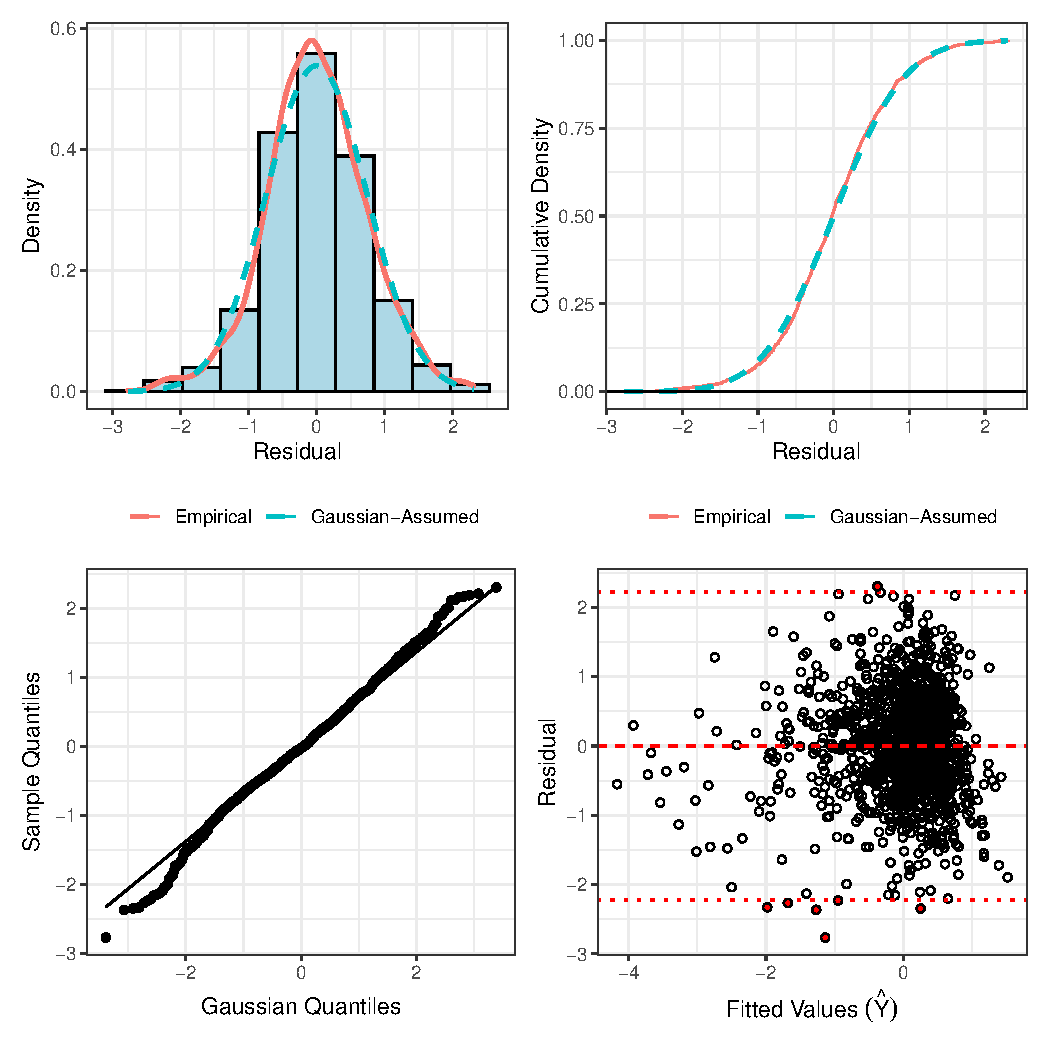
\includegraphics[width=\maxwidth]{figure/unnamed-chunk-16-1} 
\end{knitrout}
\caption{"Residual Plots of Pruned Non-Transformed Model"}
\ref{prune.resid}
\end{figure}

In our new model, according to Table \ref{pruned.first.model.un}, all remaining variables have coefficients with $p$-values $< 0.05$, indicating that the values for $\beta_i$ all fall either above or below 0. $R^2$ sees a slight decrease, but $R^2_{adj}$ is now closer to $R^2$, as $R^2 - R^2_{adj}$ goes from 0.0058 to 0.0035. Further, according to Figure \ref{prune.resid}, our residuals have remained roughly constant, compared to \ref{resid.plots.un}, and our quantile departure is approximately the same.

\begin{knitrout}
\definecolor{shadecolor}{rgb}{0.969, 0.969, 0.969}\color{fgcolor}\begin{kframe}
\begin{alltt}
\hlstd{x} \hlkwb{<-} \hlkwd{model.matrix}\hlstd{(model.2.accur)[,}\hlopt{-}\hlnum{1}\hlstd{]}

\hlstd{y} \hlkwb{<-} \hlstd{births}\hlopt{$}\hlstd{WeightLogSC}

\hlstd{xy} \hlkwb{<-} \hlkwd{as.data.frame}\hlstd{(}\hlkwd{cbind}\hlstd{(x,y))}
\hlstd{best.subsets.aic} \hlkwb{<-} \hlkwd{bestglm}\hlstd{(xy,} \hlkwc{IC}\hlstd{=}\hlstr{"AIC"}\hlstd{,} \hlkwc{TopModels} \hlstd{=} \hlnum{5}\hlstd{)}
\hlstd{best.model.aic} \hlkwb{<-} \hlstd{best.subsets.aic}\hlopt{$}\hlstd{BestModel}
\hlkwd{modelSummary}\hlstd{(best.model.aic)}
\end{alltt}
\begin{verbatim}
##                     Estimate Std. Error   t value     Pr(>|t|)
## (Intercept)       0.08513721 0.03337550  2.550889 0.0108506940
## Plural2          -1.01140649 0.11399990 -8.871994 0.0000000000
## Plural3          -1.55294830 0.35380867 -4.389232 0.0000122310
## SexMale           0.10841176 0.03699147  2.930723 0.0034367129
## MomAgeSC          0.10043150 0.02101521  4.778991 0.0000019477
## WeeksSC           0.55611048 0.02728282 20.383176 0.0000000000
## RaceMomBlack     -0.13620411 0.04749595 -2.867700 0.0041967644
## RaceMomFilipino  -1.18573278 0.69397462 -1.708611 0.0877451260
## MaritalUnmarried -0.06899117 0.04684232 -1.472838 0.1410198535
## GainedSC          0.15226585 0.01867616  8.152951 0.0000000000
## SmokeYes         -0.24364266 0.05335039 -4.566840 0.0000053871
## PreemieYes       -0.15448706 0.07933622 -1.947245 0.0517055182
## [1] "R-squared: 0.523909731643835"
## [1] "Adjusted R-Squared: 0.520160989373314"
## [1] "RMSE: 0.692704129211517"
## [1] "AIC: 2977.88217665443"
## [1] "BIC: 3046.14043830912"
## [1] "Quantile Departure: 0.157354895038271"
\end{verbatim}
\end{kframe}
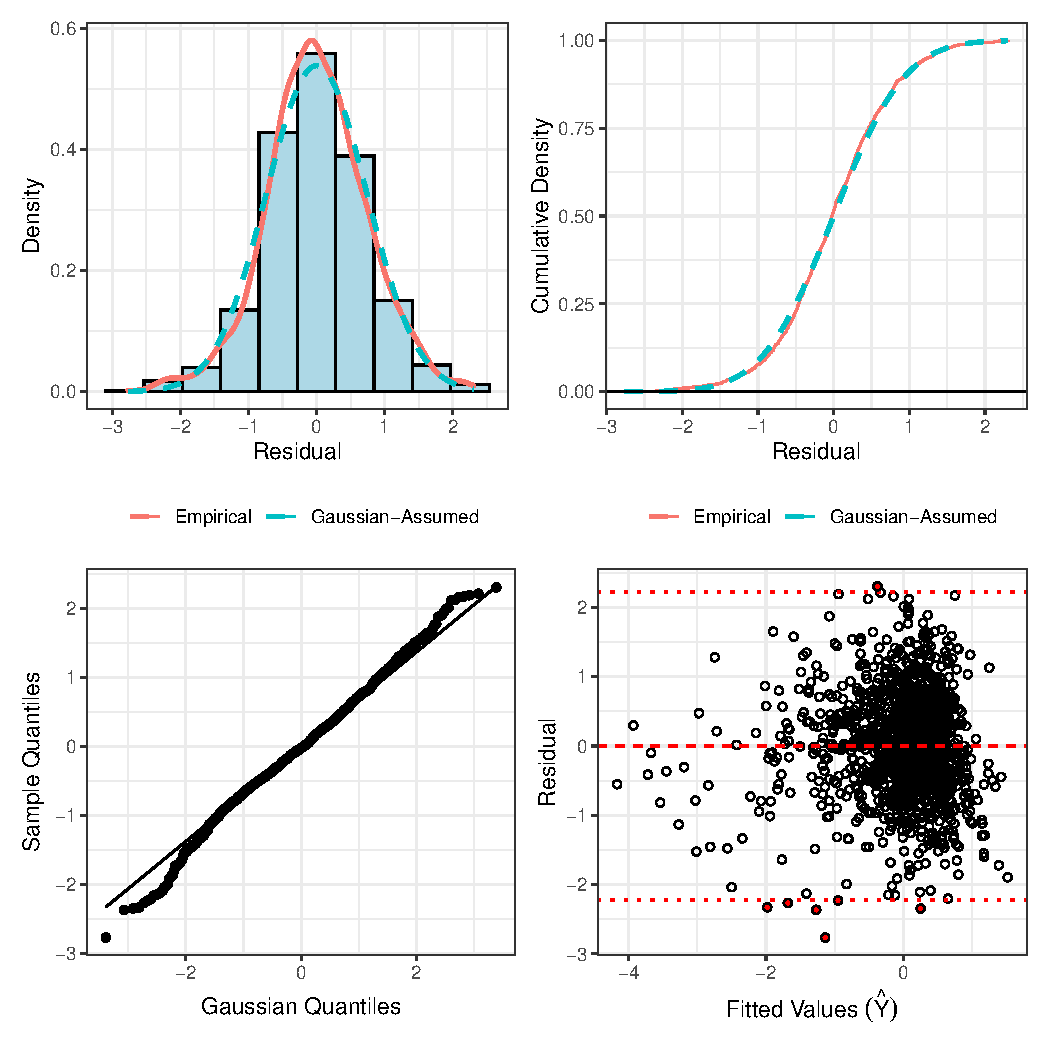
\includegraphics[width=\maxwidth]{figure/unnamed-chunk-17-1} 
\begin{kframe}\begin{alltt}
\hlstd{best.subsets.bic} \hlkwb{<-} \hlkwd{bestglm}\hlstd{(xy,} \hlkwc{IC}\hlstd{=}\hlstr{"BIC"}\hlstd{,} \hlkwc{TopModels} \hlstd{=} \hlnum{5}\hlstd{)}
\hlstd{best.model.bic} \hlkwb{<-} \hlstd{best.subsets.bic}\hlopt{$}\hlstd{BestModel}
\hlkwd{modelSummary}\hlstd{(best.model.bic)}
\end{alltt}
\begin{verbatim}
##                 Estimate Std. Error   t value     Pr(>|t|)
## (Intercept)   0.04739417 0.03001485  1.579024 0.1145563680
## Plural2      -1.03303018 0.11376403 -9.080464 0.0000000000
## Plural3      -1.59031791 0.35386995 -4.494074 0.0000075631
## SexMale       0.11093812 0.03705787  2.993645 0.0028049982
## MomAgeSC      0.11404260 0.01909745  5.971615 0.0000000030
## WeeksSC       0.59256919 0.02015023 29.407564 0.0000000000
## RaceMomBlack -0.16090779 0.04507298 -3.569939 0.0003691376
## GainedSC      0.15221554 0.01871686  8.132535 0.0000000000
## SmokeYes     -0.25749845 0.05285358 -4.871921 0.0000012309
## [1] "R-squared: 0.520773942237405"
## [1] "Adjusted R-Squared: 0.518035507621619"
## [1] "RMSE: 0.694236625638824"
## [1] "AIC: 2981.13218740264"
## [1] "BIC: 3033.63854252162"
## [1] "Quantile Departure: 0.157652048501995"
\end{verbatim}
\end{kframe}
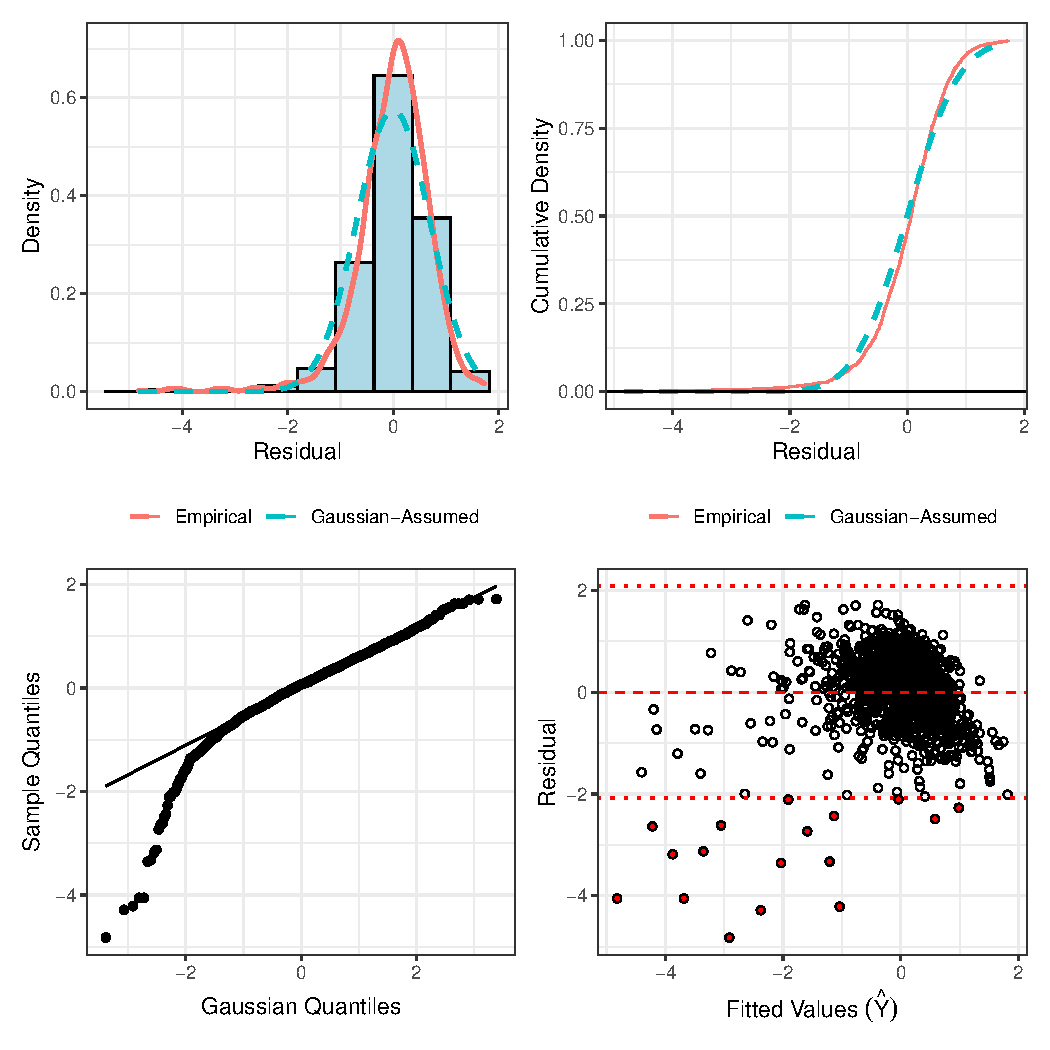
\includegraphics[width=\maxwidth]{figure/unnamed-chunk-17-2} 
\begin{kframe}\begin{alltt}
\hlstd{regsubsets.out} \hlkwb{<-} \hlkwd{regsubsets}\hlstd{(WeightLogSC} \hlopt{~} \hlstd{Plural} \hlopt{+} \hlstd{Sex} \hlopt{+} \hlstd{MomAgeSC} \hlopt{+} \hlstd{WeeksSC} \hlopt{+} \hlstd{RaceMom} \hlopt{+}
                               \hlstd{Marital} \hlopt{+} \hlstd{GainedSC} \hlopt{+} \hlstd{Smoke} \hlopt{+} \hlstd{Preemie,}
                             \hlkwc{data}\hlstd{=births,} \hlkwc{nbest} \hlstd{=} \hlnum{1}\hlstd{,} \hlkwc{nvmax}\hlstd{=}\hlnum{15}\hlstd{)}

\hlstd{fit.stats} \hlkwb{<-} \hlkwd{data.frame}\hlstd{(}\hlkwc{num.variables}\hlstd{=}\hlnum{1}\hlopt{:}\hlnum{15}\hlstd{,}
                        \hlkwc{adjr2} \hlstd{=} \hlkwd{summary}\hlstd{(regsubsets.out)}\hlopt{$}\hlstd{adjr2,}
                        \hlkwc{bic}\hlstd{=}\hlkwd{summary}\hlstd{(regsubsets.out)}\hlopt{$}\hlstd{bic)}

\hlkwd{cbind}\hlstd{(fit.stats,} \hlkwd{as.data.frame}\hlstd{(}\hlkwd{summary}\hlstd{(regsubsets.out)}\hlopt{$}\hlstd{outmat))}
\end{alltt}
\begin{verbatim}
##           num.variables     adjr2       bic Plural2 Plural3 SexMale MomAgeSC
## 1  ( 1 )              1 0.4419739 -808.4394                                 
## 2  ( 1 )              2 0.4600565 -848.6047                                 
## 3  ( 1 )              3 0.4817581 -900.1570       *                         
## 4  ( 1 )              4 0.4980496 -938.9143       *                        *
## 5  ( 1 )              5 0.5048386 -951.8545       *                        *
## 6  ( 1 )              6 0.5112379 -963.9368       *       *                *
## 7  ( 1 )              7 0.5152965 -969.4404       *       *                *
## 8  ( 1 )              8 0.5180355 -971.1805       *       *       *        *
## 9  ( 1 )              9 0.5190927 -968.0308       *       *       *        *
## 10  ( 1 )            10 0.5197597 -963.7431       *       *       *        *
## 11  ( 1 )            11 0.5201610 -958.6786       *       *       *        *
## 12  ( 1 )            12 0.5201212 -952.3202       *       *       *        *
## 13  ( 1 )            13 0.5198713 -945.3456       *       *       *        *
## 14  ( 1 )            14 0.5195516 -938.1675       *       *       *        *
## 15  ( 1 )            15 0.5192084 -930.9220       *       *       *        *
##           WeeksSC RaceMomBlack RaceMomChinese RaceMomFilipino RaceMomJapanese
## 1  ( 1 )        *                                                            
## 2  ( 1 )        *                                                            
## 3  ( 1 )        *                                                            
## 4  ( 1 )        *                                                            
## 5  ( 1 )        *                                                            
## 6  ( 1 )        *                                                            
## 7  ( 1 )        *            *                                               
## 8  ( 1 )        *            *                                               
## 9  ( 1 )        *            *                                               
## 10  ( 1 )       *            *                              *                
## 11  ( 1 )       *            *                              *                
## 12  ( 1 )       *            *                              *                
## 13  ( 1 )       *            *                              *                
## 14  ( 1 )       *            *              *               *                
## 15  ( 1 )       *            *              *               *               *
##           RaceMomOther Asian / PI RaceMomWhite MaritalUnmarried GainedSC
## 1  ( 1 )                                                                
## 2  ( 1 )                                                               *
## 3  ( 1 )                                                               *
## 4  ( 1 )                                                               *
## 5  ( 1 )                                                               *
## 6  ( 1 )                                                               *
## 7  ( 1 )                                                               *
## 8  ( 1 )                                                               *
## 9  ( 1 )                                                               *
## 10  ( 1 )                                                              *
## 11  ( 1 )                                                     *        *
## 12  ( 1 )                       *                             *        *
## 13  ( 1 )                       *            *                *        *
## 14  ( 1 )                       *            *                *        *
## 15  ( 1 )                       *            *                *        *
##           SmokeYes PreemieYes
## 1  ( 1 )                     
## 2  ( 1 )                     
## 3  ( 1 )                     
## 4  ( 1 )                     
## 5  ( 1 )         *           
## 6  ( 1 )         *           
## 7  ( 1 )         *           
## 8  ( 1 )         *           
## 9  ( 1 )         *          *
## 10  ( 1 )        *          *
## 11  ( 1 )        *          *
## 12  ( 1 )        *          *
## 13  ( 1 )        *          *
## 14  ( 1 )        *          *
## 15  ( 1 )        *          *
\end{verbatim}
\end{kframe}
\end{knitrout}

Just as with the model for the non-transformed weights, the same variables - all levels of race except for Black, as well as marital status - were recommended to be removed in the model with the $log$ transformation of the weights. Having done so, in Table \ref{pruned.first.model.log}, we found that all remaining variables were significant with $p$-values $<0.05$. 

\begin{knitrout}
\definecolor{shadecolor}{rgb}{0.969, 0.969, 0.969}\color{fgcolor}\begin{kframe}
\begin{alltt}
\hlstd{model.3.accur} \hlkwb{<-} \hlkwd{lm}\hlstd{(WeightLogSC} \hlopt{~} \hlstd{Twin} \hlopt{+} \hlstd{Triplet} \hlopt{+} \hlstd{Sex} \hlopt{+} \hlstd{MomAgeSC} \hlopt{+} \hlstd{WeeksSC} \hlopt{+} \hlstd{Black} \hlopt{+}
                      \hlstd{GainedSC} \hlopt{+} \hlstd{Smoke} \hlopt{+} \hlstd{Preemie, births)}

\hlkwd{xtable}\hlstd{(model.3.accur,} \hlkwc{caption}\hlstd{=}\hlstr{"Predictor Statistics and Significance for Pruned First-Order Log-Transformed Model"}\hlstd{,} \hlkwc{label}\hlstd{=}\hlstr{"pruned.first.model.log"}\hlstd{)}
\end{alltt}
\end{kframe}
\end{knitrout}
\begin{table}[H]
\centering
\begin{tabular}{rrrrr}
  \hline
 & Estimate & Std. Error & t value & Pr($>$$|$t$|$) \\ 
  \hline
(Intercept) & 0.0671 & 0.0315 & 2.13 & 0.0336 \\ 
  Twin & -1.0119 & 0.1141 & -8.87 & 0.0000 \\ 
  Triplet & -1.5454 & 0.3542 & -4.36 & 0.0000 \\ 
  Male & 0.1100 & 0.0370 & 2.97 & 0.0030 \\ 
  MomAge (SC) & 0.1120 & 0.0191 & 5.86 & 0.0000 \\ 
  Weeks (SC) & 0.5553 & 0.0273 & 20.33 & 0.0000 \\ 
  Black & -0.1582 & 0.0450 & -3.51 & 0.0005 \\ 
  Gained (SC) & 0.1523 & 0.0187 & 8.15 & 0.0000 \\ 
  Smoke & -0.2547 & 0.0528 & -4.82 & 0.0000 \\ 
  Preemie & -0.1602 & 0.0793 & -2.02 & 0.0436 \\ 
   \hline
\end{tabular}
\caption{Predictor Statistics and Significance for Pruned First-Order Log-Transformed Model} 
\label{pruned.first.model.log}
\end{table}

\begin{knitrout}
\definecolor{shadecolor}{rgb}{0.969, 0.969, 0.969}\color{fgcolor}\begin{kframe}
\begin{alltt}
\hlkwd{modelSummary}\hlstd{(model.3.assu,} \hlkwc{coef}\hlstd{=F,} \hlkwc{plot}\hlstd{=F)}
\end{alltt}
\begin{verbatim}
## [1] "R-squared: 0.45431789056999"
## [1] "Adjusted R-Squared: 0.450807426678017"
## [1] "RMSE: 0.741075281818239"
## [1] "AIC: 3166.11079739794"
## [1] "BIC: 3223.86778802883"
## [1] "Quantile Departure: 0.0461987895225344"
\end{verbatim}
\end{kframe}
\end{knitrout}

Just as before, our $R^2$ values decreased as we removed values, but our $R^2_{adj}$ actually remained exactly the same, going from 0.5191 to 0.5192. \\

Using these two models, we decided to conduct run cross validation tests to make sure that the data was not simply being overfit, and that our $R^2$ and MAE values were accurate to the data as a whole. We ran cross validation on both models, using both k-fold cross validation and leave-one-out cross validation. 

\begin{knitrout}
\definecolor{shadecolor}{rgb}{0.969, 0.969, 0.969}\color{fgcolor}\begin{kframe}
\begin{alltt}
\hlstd{specs} \hlkwb{<-} \hlkwd{trainControl}\hlstd{(}\hlkwc{method}\hlstd{=}\hlstr{"LOOCV"}\hlstd{)}
\hlstd{model.cval.LOO.accur} \hlkwb{<-} \hlkwd{train}\hlstd{(WeightLogSC} \hlopt{~} \hlstd{Twin} \hlopt{+} \hlstd{Triplet} \hlopt{+} \hlstd{Sex} \hlopt{+} \hlstd{MomAgeSC} \hlopt{+} \hlstd{WeeksSC} \hlopt{+} \hlstd{Black} \hlopt{+}
                      \hlstd{GainedSC} \hlopt{+} \hlstd{Smoke} \hlopt{+} \hlstd{Preemie,} \hlkwc{data}\hlstd{=births,}
                      \hlkwc{method} \hlstd{=} \hlstr{"lm"}\hlstd{,}
                      \hlkwc{trControl} \hlstd{= specs,}
                      \hlkwc{na.action} \hlstd{= na.omit)}
\hlstd{model.cval.LOO.accur}\hlopt{$}\hlstd{results[[}\hlstr{"Method"}\hlstd{]]} \hlkwb{<-} \hlstr{"LOOCV"}

\hlstd{specs} \hlkwb{<-} \hlkwd{trainControl}\hlstd{(}\hlkwc{method}\hlstd{=}\hlstr{"CV"}\hlstd{,} \hlkwc{number}\hlstd{=}\hlnum{10}\hlstd{)}

\hlstd{model.cval.cv.accur} \hlkwb{<-} \hlkwd{train}\hlstd{(WeightLogSC} \hlopt{~} \hlstd{Twin} \hlopt{+} \hlstd{Triplet} \hlopt{+} \hlstd{Sex} \hlopt{+} \hlstd{MomAgeSC} \hlopt{+} \hlstd{WeeksSC} \hlopt{+} \hlstd{Black} \hlopt{+}
                      \hlstd{GainedSC} \hlopt{+} \hlstd{Smoke} \hlopt{+} \hlstd{Preemie,} \hlkwc{data}\hlstd{=births,}
                      \hlkwc{method} \hlstd{=} \hlstr{"lm"}\hlstd{,}
                      \hlkwc{trControl} \hlstd{= specs,}
                      \hlkwc{na.action} \hlstd{= na.omit)}
\hlstd{model.cval.cv.accur}\hlopt{$}\hlstd{results[[}\hlstr{"Method"}\hlstd{]]} \hlkwb{<-} \hlstr{"K-Fold"}

\hlkwd{rbind}\hlstd{(model.cval.LOO.accur}\hlopt{$}\hlstd{results,}
      \hlstd{model.cval.cv.accur}\hlopt{$}\hlstd{results} \hlopt \hlkwd{select}\hlstd{(intercept, RMSE, Rsquared, MAE, Method))} \hlopt
  \hlkwd{select}\hlstd{(Method, RMSE, Rsquared, MAE)} \hlopt
  \hlkwd{xtable}\hlstd{(}\hlkwc{caption}\hlstd{=}\hlstr{"Comparison of Cross-Validation Techniques on Logarithmic Model"}\hlstd{,} \hlkwc{label}\hlstd{=}\hlstr{"cross.val.log"}\hlstd{)}
\end{alltt}
\end{kframe}
\end{knitrout}
\begin{table}[H]
\centering
\begin{tabular}{lrrr}
  \hline
  Method & RMSE & $R^2$ & MAE \\ 
  \hline
  None & 0.69 & 0.52 & 0.49 \\
  LOOCV & 0.70 & 0.51 & 0.50 \\ 
  K-Fold & 0.69 & 0.49 & 0.50 \\ 
   \hline
\end{tabular}
\caption{Comparison of Cross-Validation Techniques on Logarithmic Model} 
\label{cross.val.log}
\end{table}

\begin{knitrout}
\definecolor{shadecolor}{rgb}{0.969, 0.969, 0.969}\color{fgcolor}\begin{kframe}
\begin{alltt}
\hlstd{specs} \hlkwb{<-} \hlkwd{trainControl}\hlstd{(}\hlkwc{method}\hlstd{=}\hlstr{"LOOCV"}\hlstd{)}
\hlstd{model.cval.LOO.assu} \hlkwb{<-} \hlkwd{train}\hlstd{(WeightGmSC} \hlopt{~} \hlstd{Twin} \hlopt{+} \hlstd{Triplet} \hlopt{+} \hlstd{Sex} \hlopt{+} \hlstd{MomAgeSC} \hlopt{+} \hlstd{WeeksSC} \hlopt{+} \hlstd{Black} \hlopt{+}
                      \hlstd{GainedSC} \hlopt{+} \hlstd{Smoke} \hlopt{+} \hlstd{Preemie,} \hlkwc{data}\hlstd{=births,}
                      \hlkwc{method} \hlstd{=} \hlstr{"lm"}\hlstd{,}
                      \hlkwc{trControl} \hlstd{= specs,}
                      \hlkwc{na.action} \hlstd{= na.omit)}

\hlstd{model.cval.LOO.assu}\hlopt{$}\hlstd{results[[}\hlstr{"Name"}\hlstd{]]} \hlkwb{<-} \hlstr{"LOOCV"}


\hlstd{specs} \hlkwb{<-} \hlkwd{trainControl}\hlstd{(}\hlkwc{method}\hlstd{=}\hlstr{"CV"}\hlstd{,} \hlkwc{number}\hlstd{=}\hlnum{10}\hlstd{)}

\hlstd{model.cval.cv.assu} \hlkwb{<-} \hlkwd{train}\hlstd{(WeightGmSC} \hlopt{~} \hlstd{Twin} \hlopt{+} \hlstd{Triplet} \hlopt{+} \hlstd{Sex} \hlopt{+} \hlstd{MomAgeSC} \hlopt{+} \hlstd{WeeksSC} \hlopt{+} \hlstd{Black} \hlopt{+}
                      \hlstd{GainedSC} \hlopt{+} \hlstd{Smoke} \hlopt{+} \hlstd{Preemie,} \hlkwc{data}\hlstd{=births,}
                      \hlkwc{method} \hlstd{=} \hlstr{"lm"}\hlstd{,}
                      \hlkwc{trControl} \hlstd{= specs,}
                      \hlkwc{na.action} \hlstd{= na.omit)}
\hlstd{model.cval.cv.assu}\hlopt{$}\hlstd{results[[}\hlstr{"Name"}\hlstd{]]} \hlkwb{<-} \hlstr{"K-Fold"}

\hlkwd{rbind}\hlstd{(model.cval.LOO.assu}\hlopt{$}\hlstd{results,}
      \hlstd{model.cval.cv.assu}\hlopt{$}\hlstd{results} \hlopt \hlkwd{select}\hlstd{(intercept, RMSE, Rsquared, MAE, Name))} \hlopt
    \hlkwd{select}\hlstd{(RMSE, Rsquared, MAE, Name)} \hlopt
  \hlkwd{xtable}\hlstd{(}\hlkwc{caption}\hlstd{=}\hlstr{"Comparison of Cross-Validation Techniques"}\hlstd{,} \hlkwc{label}\hlstd{=}\hlstr{"cross.val.un"}\hlstd{)}
\end{alltt}
\end{kframe}
\end{knitrout}

\begin{table}[H]
\centering
\begin{tabular}{lrrr}
  \hline
 Method & RMSE & $R^2$ & MAE \\ 
  \hline
  Orig. & 0.74 & 0.45 & 0.57 \\
LOOCV & 0.74 & 0.45 & 0.58 \\ 
  K-Fold & 0.74 & 0.44 & 0.58 \\ 
   \hline
\end{tabular}
\caption{Comparison of Cross-Validation Techniques} 
\label{cross.val.un}
\end{table}

In both Table \ref{cross.val.log} and \ref{cross.val.un}, it is apparent that the cross validation yields values of RMSE, $R^2$, and MAE that are directly in line with the values we calculate using the full training data. \\

After obtaining our new model, we were curious as to how some of the predictors influenced the data set. Premature births means that the baby was born weeks before the predicted due date, and its commonly known that "Preemies" have low birth weights. They are also some of the more important subject to have accurate weight predictions of, because of their often-delicate health condition and the importance that greater levels of development can bring with it. We calculated the residuals of our models for the entire dataset, just the premature births, and just the non-premature births, and created plots comparing the distribution of residuals for each of the subsets of the data. 

\begin{figure}
\begin{knitrout}
\definecolor{shadecolor}{rgb}{0.969, 0.969, 0.969}\color{fgcolor}\begin{kframe}
\begin{alltt}
\hlkwd{predictForSubsets}\hlstd{(model.3.assu,} \hlstr{"WeightGmSC"}\hlstd{,}
                  \hlstd{births,}
                  \hlstd{births} \hlopt \hlkwd{filter}\hlstd{(Preemie}\hlopt{==}\hlstr{"Yes"}\hlstd{),}
                  \hlstd{births} \hlopt \hlkwd{filter}\hlstd{(Preemie}\hlopt{==}\hlstr{"No"}\hlstd{),}
                  \hlkwc{names}\hlstd{=}\hlkwd{c}\hlstd{(}\hlstr{"Full"}\hlstd{,} \hlstr{"Prememie"}\hlstd{,} \hlstr{"Non-Preemie"}\hlstd{))}
\end{alltt}
\begin{verbatim}
## [1] "Full R-Squared: 0.45431789056999"
## [1] "Full Mean Abs. Error: 0.573294283532389"
## [1] "Prememie R-Squared: 0.552153428004115"
## [1] "Prememie Mean Abs. Error: 0.711899847961804"
## [1] "Non-Preemie R-Squared: 0.170621641846955"
## [1] "Non-Preemie Mean Abs. Error: 0.552864636006555"
\end{verbatim}
\end{kframe}
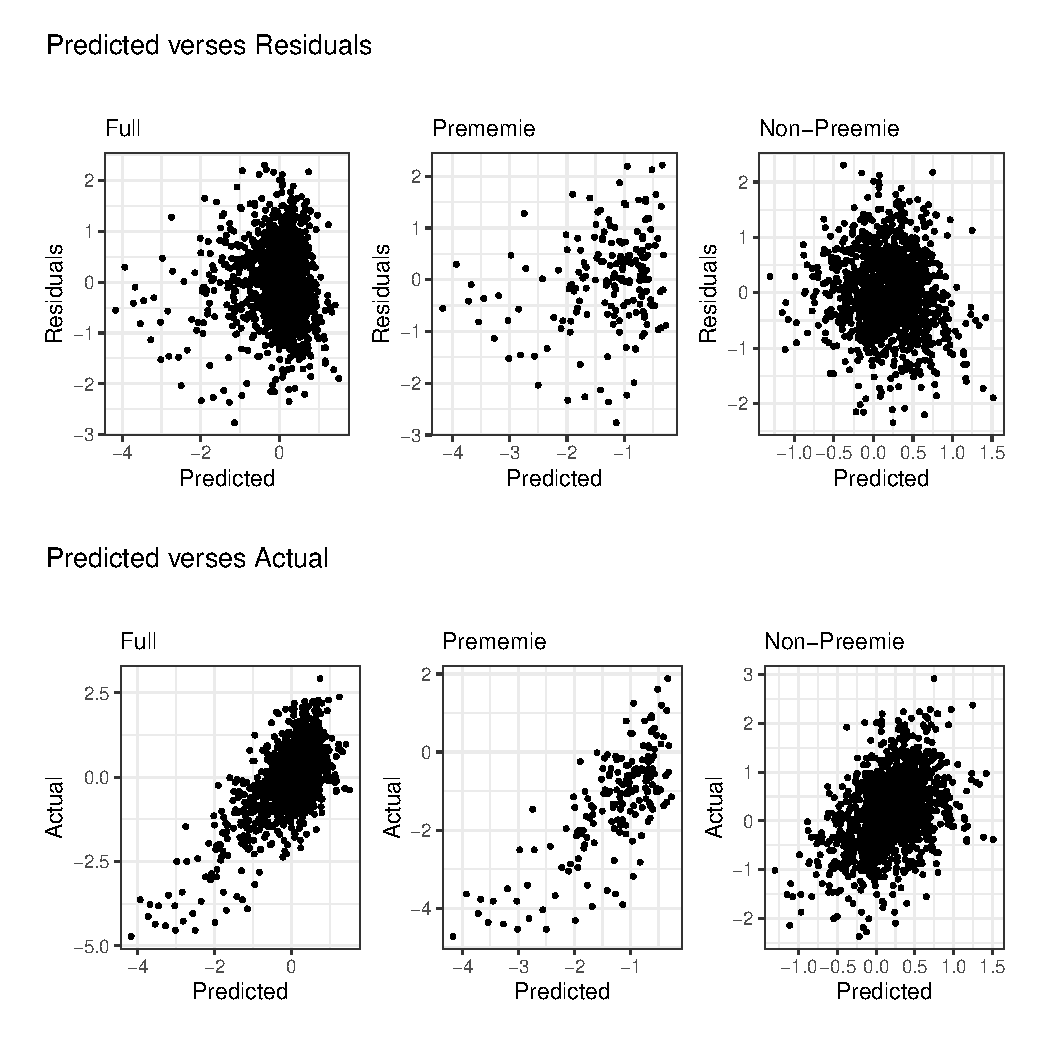
\includegraphics[width=\maxwidth]{figure/unnamed-chunk-22-1} 
\end{knitrout}
\caption{Comparison of Residual Distributions Between Datasets for Untransformed Model}
\label{resid.3.un}
\end{figure}

\begin{figure}
\begin{knitrout}
\definecolor{shadecolor}{rgb}{0.969, 0.969, 0.969}\color{fgcolor}\begin{kframe}
\begin{alltt}
\hlkwd{predictForSubsets}\hlstd{(model.3.accur,} \hlstr{"WeightLogSC"}\hlstd{,}
                  \hlstd{births,}
                  \hlstd{births} \hlopt \hlkwd{filter}\hlstd{(Preemie}\hlopt{==}\hlstr{"Yes"}\hlstd{),}
                  \hlstd{births} \hlopt \hlkwd{filter}\hlstd{(Preemie}\hlopt{==}\hlstr{"No"}\hlstd{),}
                  \hlkwc{names}\hlstd{=}\hlkwd{c}\hlstd{(}\hlstr{"Full"}\hlstd{,} \hlstr{"Prememie"}\hlstd{,} \hlstr{"Non-Preemie"}\hlstd{))}
\end{alltt}
\begin{verbatim}
## [1] "Full R-Squared: 0.522166711514882"
## [1] "Full Mean Abs. Error: 0.49562928262236"
## [1] "Prememie R-Squared: 0.655924407199486"
## [1] "Prememie Mean Abs. Error: 0.88679249101233"
## [1] "Non-Preemie R-Squared: 0.149090511038704"
## [1] "Non-Preemie Mean Abs. Error: 0.437974119170743"
\end{verbatim}
\end{kframe}
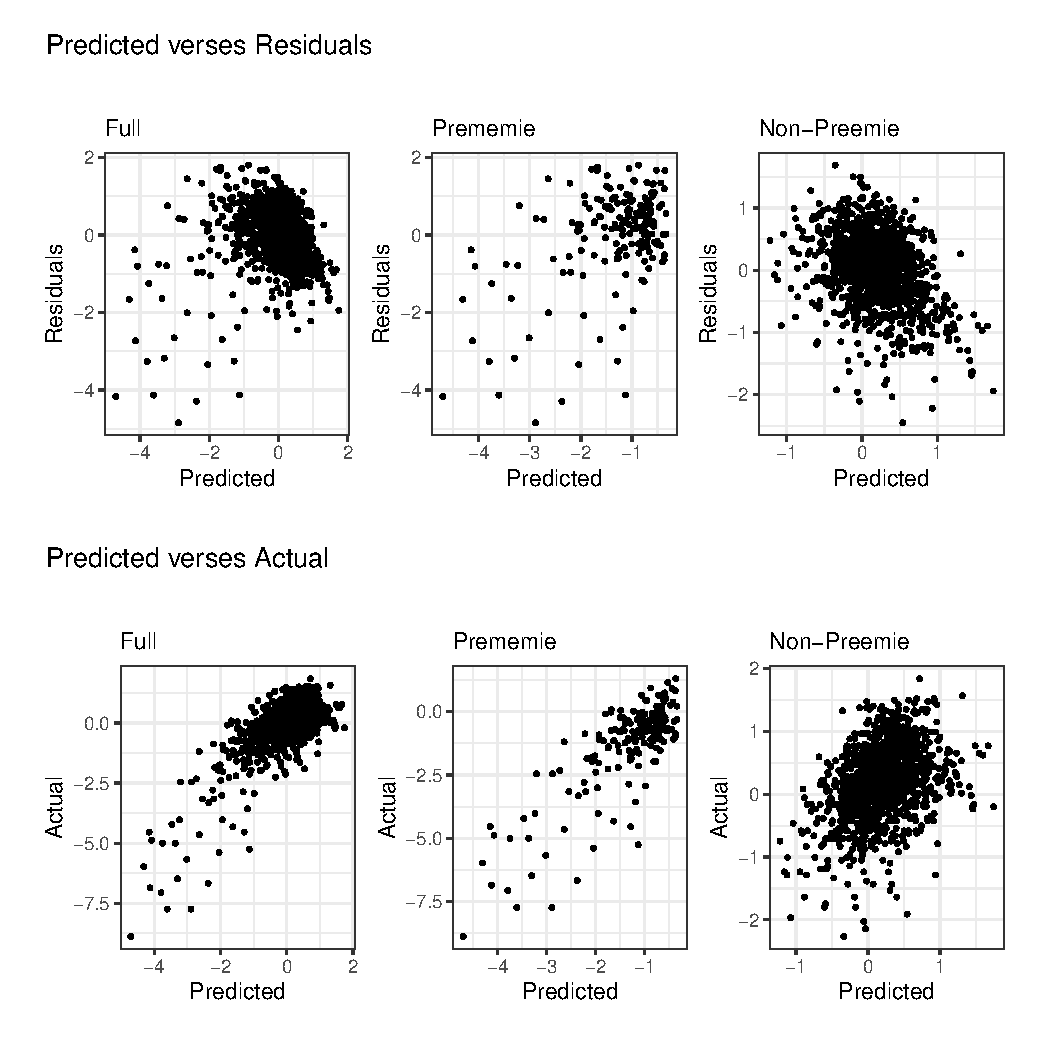
\includegraphics[width=\maxwidth]{figure/unnamed-chunk-23-1} 
\end{knitrout}
\caption{Comparison of Residual Distributions Between Subsets for Logarithmic Model}
\label{resid.3.log}
\end{figure}

As Figures \ref{resid.3.un} and \ref{resid.3.log} demonstrate, both model tend to have higher residual departures for premature births than they do for the dataset as a whole or for the subset of non-premature births. This is also reflected in the MAE values, as seen in Table \ref{subset.comp}, where the premature birth subset is always lower than the non-premature birth or the full dataset. However, Table \ref{subset.comp} also shows that premature births also have a much higher correlation with the predicted values from the model, meaning that in some sense they are both more predictive of the general trends in premature birth weights than of non-premature birth weights. Further, the logarithmic model is much better at predicting births that are at the higher ends of the weight range than at the lower end of the range, while the non-transformed model is more consistent across weight ranges. 

\begin{table}[H]
\centering
\begin{tabular}{lrrrr}
  \hline
  &  \multicolumn{2}{c}{$R^2$} & \multicolumn{2}{c}{MAE}\\
  Subset & Orig. & $log$ & Orig. & $log$\\ 
  \hline
   Births & 0.4543 & 0.5221 & 0.5732 & 0.4956 \\ 
   Preemies & 0.5521 &  0.6559 & 0.7119 &  0.8867 \\ 
   Not Preemies & 0.1706 & 0.1490 & 0.5528& 0.4380 \\
   \hline
\end{tabular}
\caption{Summary of Comparison Between Subset Evalution of Nontransformed and Logarithmic Models}
\label{subset.comp}
\end{table}

\subsection{Interaction Model}

Our next goal was to see if we could improve accuracy by fitting a full interaction model. Since the assumptions model is intended to be used for interpreting the regression term coefficients, we decided that we would only fit interaction for the accuracy-optimization model. Fitting the full interaction model yielded the following: 

\begin{knitrout}
\definecolor{shadecolor}{rgb}{0.969, 0.969, 0.969}\color{fgcolor}\begin{kframe}
\begin{alltt}
\hlstd{model.interact.accur} \hlkwb{<-} \hlkwd{lm}\hlstd{(WeightLogSC} \hlopt{~} \hlstd{(Plural} \hlopt{+} \hlstd{Sex} \hlopt{+} \hlstd{MomAgeSC} \hlopt{+} \hlstd{WeeksSC} \hlopt{+} \hlstd{Black} \hlopt{+}
                             \hlstd{GainedSC} \hlopt{+} \hlstd{Smoke} \hlopt{+} \hlstd{Preemie)}\hlopt{^}\hlnum{2}\hlstd{, births)}

\hlkwd{xtable}\hlstd{(model.interact.accur,} \hlkwc{caption}\hlstd{=}\hlstr{"Predictor Statistics and Significance for Log-Transformed Interaction Model"}\hlstd{,} \hlkwc{label}\hlstd{=}\hlstr{"interact.model.log"}\hlstd{)}
\end{alltt}
\end{kframe}
\end{knitrout}
\begin{table}[H]
\centering
\begin{tabular}{rrrrr}
  \hline
 & Estimate & Std. Error & t value & Pr($>$$|$t$|$) \\ 
  \hline
(Intercept) & 0.1686 & 0.0324 & 5.21 & 0.0000 \\ 
  Twin & -1.2867 & 0.2003 & -6.42 & 0.0000 \\ 
  Triplet & -1.6956 & 1.6094 & -1.05 & 0.2923 \\ 
  Male & 0.1304 & 0.0432 & 3.02 & 0.0026 \\ 
  MomAge (SC) & 0.0955 & 0.0278 & 3.43 & 0.0006 \\ 
  Weeks (SC) & 0.1804 & 0.0410 & 4.40 & 0.0000 \\ 
  Black & -0.1775 & 0.0632 & -2.81 & 0.0050 \\ 
  Gained (SC) & 0.1436 & 0.0282 & 5.08 & 0.0000 \\ 
  Smoke & -0.2597 & 0.0780 & -3.33 & 0.0009 \\ 
  Preemie & 0.8388 & 0.1400 & 5.99 & 0.0000 \\ 
  Twin:Male & 0.1786 & 0.2021 & 0.88 & 0.3770 \\ 
  Triplet:Male & 0.5711 & 0.8682 & 0.66 & 0.5108 \\ 
  Twin:MomAge (SC) & -0.0038 & 0.1098 & -0.03 & 0.9725 \\ 
  Triplet:MomAge (SC) & 0.1514 & 1.0843 & 0.14 & 0.8890 \\ 
  Twin:Weeks (SC) & -0.2927 & 0.1009 & -2.90 & 0.0038 \\ 
  Triplet:Weeks (SC) & -0.2034 & 0.2702 & -0.75 & 0.4518 \\ 
  Twin:Black & -0.3361 & 0.3158 & -1.06 & 0.2873 \\ 
  Twin:Gained (SC) & -0.0882 & 0.0954 & -0.92 & 0.3554 \\ 
  Twin:Smoke & 0.3392 & 0.5266 & 0.64 & 0.5196 \\ 
  Twin:Preemie & 0.0904 & 0.2789 & 0.32 & 0.7458 \\ 
  Male:MomAge (SC) & 0.0140 & 0.0330 & 0.42 & 0.6723 \\ 
  Male:Weeks (SC) & -0.0221 & 0.0497 & -0.44 & 0.6568 \\ 
  Male:Black & -0.0883 & 0.0778 & -1.13 & 0.2566 \\ 
  Male:Gained (SC) & 0.0139 & 0.0326 & 0.43 & 0.6699 \\ 
  Male:Smoke & -0.0280 & 0.0927 & -0.30 & 0.7629 \\ 
  Male:Preemie & -0.0164 & 0.1385 & -0.12 & 0.9056 \\ 
  MomAge (SC):Weeks (SC) & 0.0003 & 0.0256 & 0.01 & 0.9905 \\ 
  MomAge (SC):Black & -0.0342 & 0.0399 & -0.86 & 0.3916 \\ 
  MomAge (SC):Gained (SC) & -0.0041 & 0.0174 & -0.23 & 0.8157 \\ 
  MomAge (SC):Smoke & -0.1053 & 0.0474 & -2.22 & 0.0265 \\ 
  MomAge (SC):Preemie & -0.0329 & 0.0697 & -0.47 & 0.6371 \\ 
  Weeks (SC):Black & 0.1516 & 0.0545 & 2.78 & 0.0055 \\ 
  Weeks (SC):Gained (SC) & -0.0641 & 0.0250 & -2.56 & 0.0105 \\ 
  Weeks (SC):Smoke & -0.1369 & 0.0627 & -2.18 & 0.0293 \\ 
  Weeks (SC):Preemie & 1.1095 & 0.0663 & 16.74 & 0.0000 \\ 
  Black:Gained (SC) & -0.0330 & 0.0372 & -0.89 & 0.3759 \\ 
  Black:Smoke & 0.1584 & 0.1152 & 1.37 & 0.1694 \\ 
  Black:Preemie & 0.5377 & 0.1605 & 3.35 & 0.0008 \\ 
  Gained (SC):Smoke & -0.0404 & 0.0433 & -0.93 & 0.3507 \\ 
  Gained (SC):Preemie & -0.0642 & 0.0761 & -0.84 & 0.3992 \\ 
  Smoke:Preemie & 0.0710 & 0.1898 & 0.37 & 0.7083 \\ 
   \hline
\end{tabular}
\caption{Predictor Statistics and Significance for Log-Transformed Interaction Model} 
\label{interact.model.log}
\end{table}
\begin{knitrout}
\definecolor{shadecolor}{rgb}{0.969, 0.969, 0.969}\color{fgcolor}\begin{kframe}
\begin{alltt}
\hlkwd{modelSummary}\hlstd{(model.interact.accur,} \hlkwc{coef}\hlstd{=F,} \hlkwc{plot}\hlstd{=F)}
\end{alltt}


{\ttfamily\noindent\bfseries\color{errorcolor}{\#\# Error in summary(model): object 'model.interact.accur' not found}}\end{kframe}
\end{knitrout}

The accuracy of this model is much improved; our $R^2$ value is nearly 30\% higher than it was previously, and our RMSE, AIC and BIC values each have seen modest improvements. However, there are far too many terms, leading to a much lower proportion of significant estimations for the linear regression coefficients, and pruning is necessary to reduce the size of the model to only the most important terms.

\subsection{Interaction Model Pruning}

To prune our interaction model, we used the step-wise reduction method to reduce terms on the basis of AIC values. Doing so yields the following model:

\begin{knitrout}
\definecolor{shadecolor}{rgb}{0.969, 0.969, 0.969}\color{fgcolor}\begin{kframe}
\begin{alltt}
\hlkwd{step}\hlstd{(model.interact.accur,} \hlkwc{direction}\hlstd{=}\hlstr{"both"}\hlstd{)}
\end{alltt}
\end{kframe}
\end{knitrout}
\begin{knitrout}
\definecolor{shadecolor}{rgb}{0.969, 0.969, 0.969}\color{fgcolor}\begin{kframe}
\begin{alltt}
\hlstd{step.reduced.accur} \hlkwb{<-} \hlkwd{lm}\hlstd{(}\hlkwc{formula} \hlstd{= WeightLogSC} \hlopt{~} \hlstd{Twin} \hlopt{+} \hlstd{Triplet} \hlopt{+} \hlstd{Sex} \hlopt{+} \hlstd{MomAgeSC} \hlopt{+} \hlstd{WeeksSC} \hlopt{+}
                  \hlstd{Black} \hlopt{+} \hlstd{GainedSC} \hlopt{+} \hlstd{Smoke} \hlopt{+} \hlstd{Preemie} \hlopt{+} \hlstd{Twin}\hlopt{:}\hlstd{WeeksSC} \hlopt{+} \hlstd{Triplet}\hlopt{:}\hlstd{WeeksSC} \hlopt{+} \hlstd{MomAgeSC}\hlopt{:}\hlstd{Smoke} \hlopt{+}
                  \hlstd{WeeksSC}\hlopt{:}\hlstd{Black} \hlopt{+} \hlstd{WeeksSC}\hlopt{:}\hlstd{GainedSC} \hlopt{+} \hlstd{WeeksSC}\hlopt{:}\hlstd{Smoke} \hlopt{+} \hlstd{WeeksSC}\hlopt{:}\hlstd{Preemie} \hlopt{+}
                  \hlstd{Black}\hlopt{:}\hlstd{Smoke} \hlopt{+} \hlstd{Black}\hlopt{:}\hlstd{Preemie,} \hlkwc{data} \hlstd{= births)}
\hlkwd{xtable}\hlstd{(step.reduced.accur,} \hlkwc{caption}\hlstd{=}\hlstr{"Predictor Statistics and Significance for Log-Transformed Pruned Interaction Model"}\hlstd{,} \hlkwc{label}\hlstd{=}\hlstr{"interact.model.log.prune"}\hlstd{)}
\end{alltt}
\end{kframe}
\end{knitrout}
\begin{table}[H]
\centering
\begin{tabular}{rrrrr}
  \hline
 & Estimate & Std. Error & t value & Pr($>$$|$t$|$) \\ 
  \hline
(Intercept) & 0.1813 & 0.0279 & 6.49 & 0.0000 \\ 
  Twin & -1.2273 & 0.1369 & -8.97 & 0.0000 \\ 
  Triplet & -1.0309 & 0.6270 & -1.64 & 0.1004 \\ 
  Male & 0.1110 & 0.0316 & 3.51 & 0.0005 \\ 
  MomAge (SC) & 0.0912 & 0.0178 & 5.14 & 0.0000 \\ 
  Weeks (SC) & 0.1688 & 0.0321 & 5.26 & 0.0000 \\ 
  Black & -0.2197 & 0.0471 & -4.66 & 0.0000 \\ 
  Gained (SC) & 0.1250 & 0.0160 & 7.80 & 0.0000 \\ 
  Smoke & -0.2696 & 0.0516 & -5.22 & 0.0000 \\ 
  Preemie & 0.8473 & 0.1045 & 8.10 & 0.0000 \\ 
  Twin:Weeks (SC) & -0.2970 & 0.0700 & -4.25 & 0.0000 \\ 
  Triplet:Weeks (SC) & -0.0969 & 0.2116 & -0.46 & 0.6470 \\ 
  MomAge (SC):Smoke & -0.1005 & 0.0466 & -2.16 & 0.0313 \\ 
  Weeks (SC):Black & 0.1588 & 0.0521 & 3.05 & 0.0023 \\ 
  Weeks (SC):Gained (SC) & -0.0422 & 0.0169 & -2.50 & 0.0127 \\ 
  Weeks (SC):Smoke & -0.1502 & 0.0422 & -3.56 & 0.0004 \\ 
  Weeks (SC):Preemie & 1.1080 & 0.0601 & 18.45 & 0.0000 \\ 
  Black:Smoke & 0.1590 & 0.1121 & 1.42 & 0.1564 \\ 
  Black:Preemie & 0.5283 & 0.1537 & 3.44 & 0.0006 \\ 
   \hline
\end{tabular}
\caption{Predictor Statistics and Significance for Log-Transformed Pruned Interaction Model} 
\label{interact.model.log.prune}
\end{table}
\begin{knitrout}
\definecolor{shadecolor}{rgb}{0.969, 0.969, 0.969}\color{fgcolor}\begin{kframe}
\begin{alltt}
\hlkwd{modelSummary}\hlstd{(step.reduced.accur,} \hlkwc{coef}\hlstd{=F,} \hlkwc{plot}\hlstd{=F)}
\end{alltt}
\begin{verbatim}
## [1] "R-squared: 0.655809585063165"
## [1] "Adjusted R-Squared: 0.651352442999235"
## [1] "RMSE: 0.59046384902106"
## [1] "AIC: 2534.78504921359"
## [1] "BIC: 2639.79775945157"
## [1] "Quantile Departure: 0.0933319382706169"
\end{verbatim}
\end{kframe}
\end{knitrout}

This leaves us with a total of 18 regression attributes with associated estimated linear regression coefficients, of which all but 3 have significant $p$-values. 

\begin{knitrout}
\definecolor{shadecolor}{rgb}{0.969, 0.969, 0.969}\color{fgcolor}\begin{kframe}
\begin{alltt}
\hlstd{specs} \hlkwb{<-} \hlkwd{trainControl}\hlstd{(}\hlkwc{method}\hlstd{=}\hlstr{"LOOCV"}\hlstd{)}
\hlstd{model.cval.LOO} \hlkwb{<-} \hlkwd{train}\hlstd{( WeightLogSC} \hlopt{~} \hlstd{Twin} \hlopt{+} \hlstd{Triplet} \hlopt{+} \hlstd{Sex} \hlopt{+} \hlstd{MomAgeSC} \hlopt{+} \hlstd{WeeksSC} \hlopt{+}
                  \hlstd{Black} \hlopt{+} \hlstd{GainedSC} \hlopt{+} \hlstd{Smoke} \hlopt{+} \hlstd{Preemie} \hlopt{+} \hlstd{Twin}\hlopt{:}\hlstd{WeeksSC} \hlopt{+} \hlstd{Triplet}\hlopt{:}\hlstd{WeeksSC} \hlopt{+} \hlstd{MomAgeSC}\hlopt{:}\hlstd{Smoke} \hlopt{+}
                  \hlstd{WeeksSC}\hlopt{:}\hlstd{Black} \hlopt{+} \hlstd{WeeksSC}\hlopt{:}\hlstd{GainedSC} \hlopt{+} \hlstd{WeeksSC}\hlopt{:}\hlstd{Smoke} \hlopt{+} \hlstd{WeeksSC}\hlopt{:}\hlstd{Preemie} \hlopt{+}
                  \hlstd{Black}\hlopt{:}\hlstd{Smoke} \hlopt{+} \hlstd{Black}\hlopt{:}\hlstd{Preemie,} \hlkwc{data}\hlstd{=births,}
                      \hlkwc{method} \hlstd{=} \hlstr{"lm"}\hlstd{,}
                      \hlkwc{trControl} \hlstd{= specs,}
                      \hlkwc{na.action} \hlstd{= na.omit)}
\hlstd{model.cval.LOO}\hlopt{$}\hlstd{results[[}\hlstr{"Method"}\hlstd{]]} \hlkwb{<-} \hlstr{"LOOCV"}

\hlstd{specs} \hlkwb{<-} \hlkwd{trainControl}\hlstd{(}\hlkwc{method}\hlstd{=}\hlstr{"CV"}\hlstd{,} \hlkwc{number}\hlstd{=}\hlnum{10}\hlstd{)}

\hlstd{model.cval.cv} \hlkwb{<-} \hlkwd{train}\hlstd{( WeightLogSC} \hlopt{~} \hlstd{Twin} \hlopt{+} \hlstd{Triplet} \hlopt{+} \hlstd{Sex} \hlopt{+} \hlstd{MomAgeSC} \hlopt{+} \hlstd{WeeksSC} \hlopt{+}
                  \hlstd{Black} \hlopt{+} \hlstd{GainedSC} \hlopt{+} \hlstd{Smoke} \hlopt{+} \hlstd{Preemie} \hlopt{+} \hlstd{Twin}\hlopt{:}\hlstd{WeeksSC} \hlopt{+} \hlstd{Triplet}\hlopt{:}\hlstd{WeeksSC} \hlopt{+} \hlstd{MomAgeSC}\hlopt{:}\hlstd{Smoke} \hlopt{+}
                  \hlstd{WeeksSC}\hlopt{:}\hlstd{Black} \hlopt{+} \hlstd{WeeksSC}\hlopt{:}\hlstd{GainedSC} \hlopt{+} \hlstd{WeeksSC}\hlopt{:}\hlstd{Smoke} \hlopt{+} \hlstd{WeeksSC}\hlopt{:}\hlstd{Preemie} \hlopt{+}
                  \hlstd{Black}\hlopt{:}\hlstd{Smoke} \hlopt{+} \hlstd{Black}\hlopt{:}\hlstd{Preemie,} \hlkwc{data}\hlstd{=births,}
                      \hlkwc{method} \hlstd{=} \hlstr{"lm"}\hlstd{,}
                      \hlkwc{trControl} \hlstd{= specs,}
                      \hlkwc{na.action} \hlstd{= na.omit)}
\hlstd{model.cval.cv}\hlopt{$}\hlstd{results[[}\hlstr{"Method"}\hlstd{]]} \hlkwb{<-} \hlstr{"K-Fold"}

\hlkwd{rbind}\hlstd{(model.cval.LOO}\hlopt{$}\hlstd{results,}
      \hlstd{model.cval.cv}\hlopt{$}\hlstd{results} \hlopt \hlkwd{select}\hlstd{(intercept, RMSE, Rsquared, MAE, Method))} \hlopt
  \hlkwd{select}\hlstd{(Method, RMSE, Rsquared, MAE)} \hlopt
  \hlkwd{xtable}\hlstd{(}\hlkwc{caption}\hlstd{=}\hlstr{"Comparison of Cross-Validation Techniques on Logarithmic Model"}\hlstd{,} \hlkwc{label}\hlstd{=}\hlstr{"cross.val.log"}\hlstd{)}
\end{alltt}
\end{kframe}
\end{knitrout}

\begin{table}[H]
\centering
\begin{tabular}{lrrr}
  \hline
 Method & RMSE & $R^2$ & MAE \\ 
  \hline
  Orig. & 0.59 & 0.66 & 0.44 \\
  LOOCV & 0.60 & 0.64 & 0.45 \\ 
  K-Fold & 0.62 & 0.61 & 0.45 \\ 
   \hline
\end{tabular}
\caption{Comparison of Cross-Validation Techniques on Logarithmic Model} 
\label{cross.val.log}
\end{table}

After conducting k-fold and leave-one-out cross validation, we find that they are in general agreement with our calculations of RMSE, $R^2$, and MAE; the k-fold cross validation has a value of $R^2$ that is somewhat lower than the original calculation and the LOOCV value, but not by much, and at a level that is still much higher than our original model. \\

Similar to our estimates with the earlier model, we wanted to see how the model performed on the three sections of the dataset, our full dataset, the premature births, and the non-premature births. 

\begin{figure}
\begin{knitrout}
\definecolor{shadecolor}{rgb}{0.969, 0.969, 0.969}\color{fgcolor}\begin{kframe}
\begin{alltt}
\hlkwd{predictForSubsets}\hlstd{(step.reduced.accur,} \hlstr{"WeightLogSC"}\hlstd{,}
                  \hlstd{births,}
                  \hlstd{births} \hlopt \hlkwd{filter}\hlstd{(Preemie}\hlopt{==}\hlstr{"Yes"}\hlstd{),}
                  \hlstd{births} \hlopt \hlkwd{filter}\hlstd{(Preemie}\hlopt{==}\hlstr{"No"}\hlstd{),}
                  \hlkwc{names}\hlstd{=}\hlkwd{c}\hlstd{(}\hlstr{"Full"}\hlstd{,} \hlstr{"Prememie"}\hlstd{,} \hlstr{"Non-Preemie"}\hlstd{))}
\end{alltt}
\begin{verbatim}
## [1] "Full R-Squared: 0.655809585063165"
## [1] "Full Mean Abs. Error: 0.43790859844828"
## [1] "Prememie R-Squared: 0.739035494835646"
## [1] "Prememie Mean Abs. Error: 0.711172337610276"
## [1] "Non-Preemie R-Squared: 0.207166479655761"
## [1] "Non-Preemie Mean Abs. Error: 0.397631125493621"
\end{verbatim}
\end{kframe}
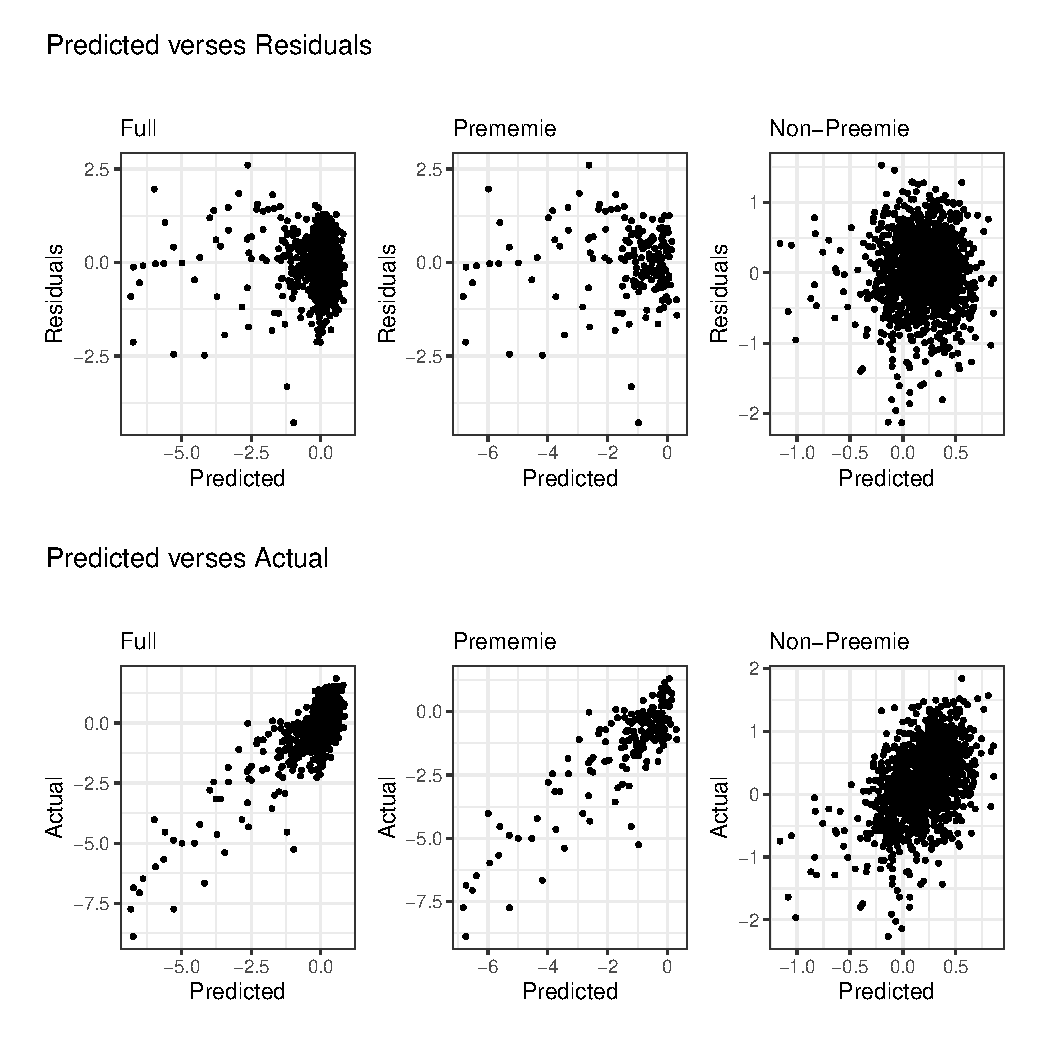
\includegraphics[width=\maxwidth]{figure/unnamed-chunk-30-1} 
\end{knitrout}
\caption{Comparison of Residual Distributions Between Subsets for Pruned Interaction Logarithmic Model}
\label{resid.final}
\end{figure}

\begin{figure}
\begin{knitrout}
\definecolor{shadecolor}{rgb}{0.969, 0.969, 0.969}\color{fgcolor}\begin{kframe}
\begin{alltt}
\hlkwd{plotResiduals}\hlstd{(step.reduced.accur)}
\end{alltt}
\end{kframe}
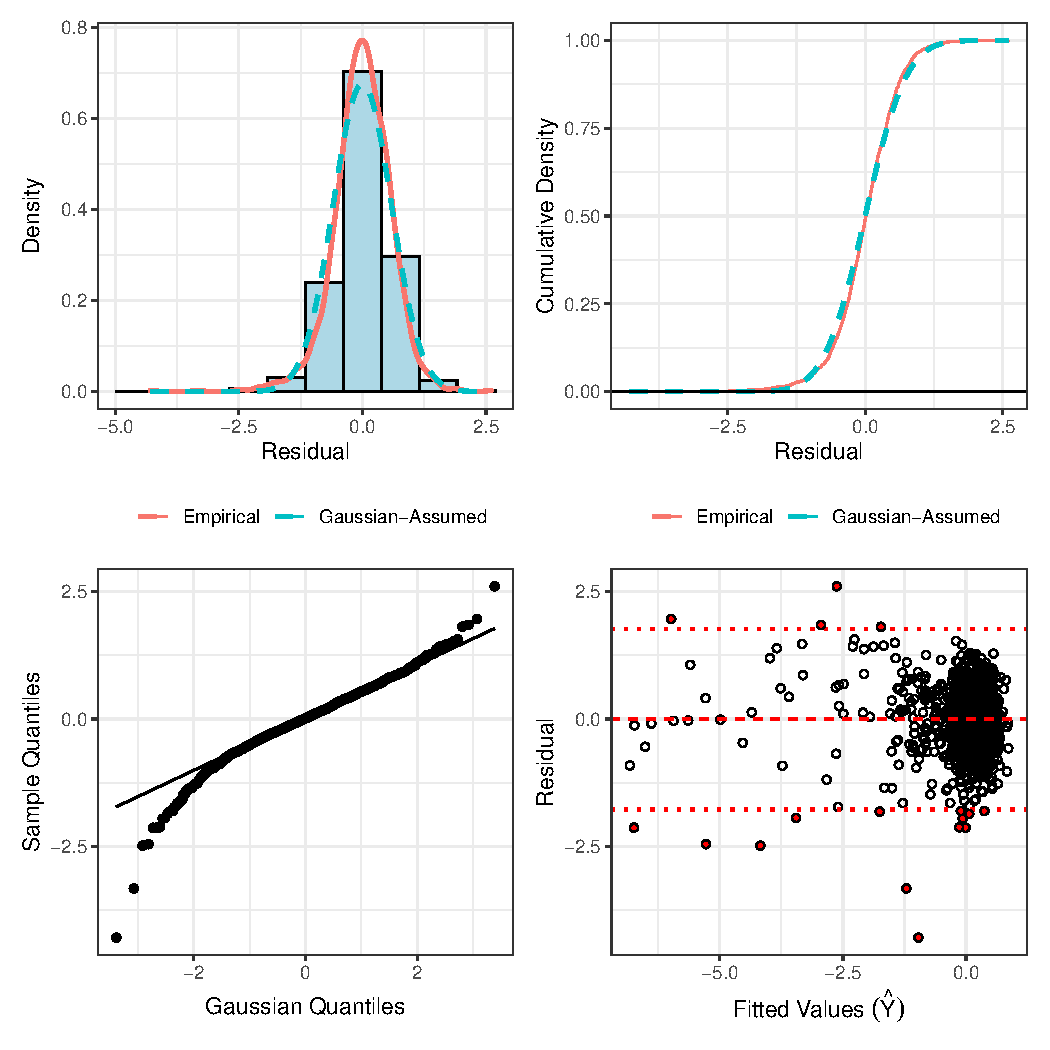
\includegraphics[width=\maxwidth]{figure/unnamed-chunk-31-1} 
\end{knitrout}
\caption{Distribution of Residuals for Pruned Interaction Logarithmic Model}
\label{resid.plots.final}
\end{figure}

As Figure \ref{resid.final} demonstrates when compared to Figure \ref{resid.3.log}, the residuals seem more evenly distributed. Premature births and birth weights around the lower end of the estimation tend to be overestimated, but predictions, especially around the main range of values, seems much more accurate, with the only notable area with large departures coming from reduction of mid-ranged values of the non-premature babies. The Residual-Density plot from Figure \ref{resid.plots.final} indicates that, if anything, residuals in the neighborhood of 0 are somewhat over-represented.

\subsection{Variance Inflation Factor Assessment}

Before finalizing our models, we checked to ensure that variance inflation did not play into the model's accurace using the VIF test. 

\begin{knitrout}
\definecolor{shadecolor}{rgb}{0.969, 0.969, 0.969}\color{fgcolor}\begin{kframe}
\begin{alltt}
\hlkwd{vif}\hlstd{(model.3.assu)} \hlopt \hlkwd{as.data.frame}\hlstd{()} \hlkwb{->} \hlstd{assu.vif}
\hlkwd{vif}\hlstd{(step.reduced.accur)} \hlopt \hlkwd{as.data.frame}\hlstd{()} \hlkwb{->} \hlstd{accur.vif}
\end{alltt}


{\ttfamily\noindent\itshape\color{messagecolor}{\#\# there are higher-order terms (interactions) in this model\\\#\# consider setting type = 'predictor'; see ?vif}}\begin{alltt}
\hlstd{assu.vif} \hlopt \hlkwd{xtable}\hlstd{(}\hlkwc{caption}\hlstd{=}\hlstr{"VIF Values for Pruned Nontransformed Regression Model"}\hlstd{,}
                    \hlkwc{label}\hlstd{=}\hlstr{"vif.val.assu"}\hlstd{)}
\hlstd{accur.vif} \hlopt  \hlkwd{xtable}\hlstd{(}\hlkwc{caption}\hlstd{=}\hlstr{"VIF Values for Pruned Logarithmic Interaction Regression Model"}\hlstd{,}
                    \hlkwc{label}\hlstd{=}\hlstr{"vif.val.accur"}\hlstd{)}
\end{alltt}
\end{kframe}
\end{knitrout}

\begin{table}[H]
\centering
\begin{tabular}{rr}
  \hline
 & VIF \\ 
  \hline
Twin & 1.13 \\ 
  Triplet & 1.04 \\ 
  Sex & 1.00 \\ 
  MomAge (SC) & 1.07 \\ 
  Weeks (SC) & 2.11 \\ 
  Black & 1.05 \\ 
  Gained (SC) & 1.02 \\ 
  Smoke & 1.02 \\ 
  Preemie & 2.06 \\ 
   \hline
\end{tabular}
\caption{VIF Values for Pruned Nontransformed Regression Model} 
\label{vif.val.assu}
\end{table}

\begin{table}[H]
\centering
\begin{tabular}{rr}
  \hline
 & VIF \\ 
  \hline
Twin & 2.24 \\ 
  Triplet & 4.50 \\ 
  Sex & 1.01 \\ 
  MomAge (SC) & 1.27 \\ 
  Weeks (SC) & 4.02 \\ 
  Black & 1.59 \\ 
  Gained (SC) & 1.04 \\ 
  Smoke & 1.34 \\ 
  Preemie & 4.95 \\ 
  Twin:Weeks (SC) & 2.98 \\ 
  Triplet:Weeks (SC) & 4.64 \\ 
  MomAge (SC) Smoke & 1.24 \\ 
  Weeks (SC) Black & 3.51 \\ 
  Weeks (SC) Gained (SC) & 1.30 \\ 
  Weeks (SC) Smoke & 1.40 \\ 
  Weeks (SC) Preemie & 7.91 \\ 
  Black:Smoke & 1.44 \\ 
  Black:Preemie & 3.64 \\ 
   \hline
\end{tabular}
\caption{VIF Values for Pruned Logarithmic Interaction Regression Model} 
\label{vif.val.accur}
\end{table}

In Table \ref{vif.val.assu}, we see that all VIF values fall below 3, and are thus very acceptable; for Table \ref{vif.val.accur}, all but one value falls below 5, which is the highly-acceptable limit, and the last remaining value still falls below 10, which is the moderatly-acceptable limit. We are thus confident that variance inflation is not a particularly heavy factor in our model, and collinearity is not a significant problem.

\section{Final Model(s) and Conclusions.}

The following are the descriptions and linear regressions of our two final models:
\begin{enumerate}
\item \textbf{step.reduced.accur}:




\item \textbf{model.3.assu}:



\begin{align*}
\hat{y} &= 0.0948 + -1.1201\cdot I(Twin = \text{TRUE}) + -1.4721\cdot I(Triplet = \text{TRUE}) + 0.1522\cdot I(Sex = \text{Male}) \\ &\quad + 0.1186\cdot \text{MomAgeSC} + 0.4187\cdot \text{WeeksSC} - 0.1917\cdot I(Black = \text{TRUE}) \\ &\quad + 0.1738\cdot \text{GainedSC} - 0.3343\cdot I(Smoke = \text{Yes}) - 0.3577\cdot I(Preemie = \text{Yes})
\end{align*}
\end{enumerate}



\begin{enumerate}[a.]
\item \textbf{Assess (and summarize) Model Diagnostics}\\
We wrote a function to perform our assumptions on one of our final models, \textbf{step.reduced.accur}, and assessed the results below.
\begin{knitrout}
\definecolor{shadecolor}{rgb}{0.969, 0.969, 0.969}\color{fgcolor}\begin{kframe}
\begin{alltt}
\hlstd{assessModel} \hlkwb{<-} \hlkwa{function}\hlstd{(}\hlkwc{model}\hlstd{,} \hlkwc{p}\hlstd{) \{}
  \hlkwd{print}\hlstd{(}\hlkwd{modelSummary}\hlstd{(model,} \hlkwc{plots}\hlstd{=F))}
  \hlkwd{cbind}\hlstd{(}\hlkwd{vif}\hlstd{(model),} \hlkwd{vif}\hlstd{(model)[,}\hlnum{3}\hlstd{]}\hlopt{^}\hlnum{2}\hlstd{)}
  \hlkwd{print}\hlstd{(}\hlkwd{summary}\hlstd{(model}\hlopt{$}\hlstd{residual))}
  \hlkwd{print}\hlstd{(}\hlkwd{confint}\hlstd{(model))}

  \hlcom{#leverage points}
  \hlstd{lev} \hlkwb{<-} \hlstd{model}\hlopt{$}\hlstd{model} \hlopt \hlkwd{mutate}\hlstd{(}\hlkwc{h.values} \hlstd{=} \hlkwd{hatvalues}\hlstd{(model))}
  \hlcom{#high leverage points }
  \hlkwd{print}\hlstd{(}\hlkwd{summary}\hlstd{(lev}\hlopt{$}\hlstd{h.values))}
  \hlstd{n} \hlkwb{<-} \hlkwd{nrow}\hlstd{(model}\hlopt{$}\hlstd{model)}
  \hlstd{high.lev} \hlkwb{<-} \hlstd{lev} \hlopt \hlkwd{filter}\hlstd{(h.values} \hlopt{>} \hlnum{2}\hlopt{*}\hlstd{p}\hlopt{/}\hlstd{n)}
  \hlkwd{print}\hlstd{(}\hlkwd{paste}\hlstd{(}\hlstr{"High Lev.:"}\hlstd{,} \hlkwd{nrow}\hlstd{(high.lev)))}
  \hlcom{#very high leverage points}
  \hlstd{v.high.lev} \hlkwb{<-} \hlstd{lev} \hlopt \hlkwd{filter}\hlstd{(h.values} \hlopt{>} \hlnum{3}\hlopt{*}\hlstd{p}\hlopt{/}\hlstd{n)}
  \hlkwd{print}\hlstd{(}\hlkwd{paste}\hlstd{(}\hlstr{"Very High Lev.:"}\hlstd{,} \hlkwd{nrow}\hlstd{(v.high.lev)))}

  \hlcom{#Stud and Stand residual quantiles }

  \hlstd{new.resid} \hlkwb{<-} \hlstd{model}\hlopt{$}\hlstd{model} \hlopt \hlkwd{mutate}\hlstd{(}\hlkwc{stdres} \hlstd{=} \hlkwd{rstandard}\hlstd{(model),}
                                      \hlkwc{stures} \hlstd{=} \hlkwd{rstudent}\hlstd{(model))}
  \hlkwd{print}\hlstd{(}\hlstr{"Standard Residual Quant.:"}\hlstd{)}
  \hlkwd{print}\hlstd{(}\hlkwd{summary}\hlstd{(new.resid}\hlopt{$}\hlstd{stdres))}
  \hlkwd{print}\hlstd{(}\hlstr{"Studentized Residual Quant.:"}\hlstd{)}
  \hlkwd{print}\hlstd{(}\hlkwd{summary}\hlstd{(new.resid}\hlopt{$}\hlstd{stures))}

  \hlcom{#outliers}
  \hlstd{s.outliers.stdres} \hlkwb{<-} \hlstd{new.resid} \hlopt \hlkwd{filter}\hlstd{(}\hlkwd{abs}\hlstd{(stdres)}\hlopt{>}\hlnum{3}\hlstd{)}
  \hlstd{(}\hlkwd{paste}\hlstd{(}\hlstr{"Strong Standard Residual Outliers:"}\hlstd{,} \hlkwd{nrow}\hlstd{(s.outliers.stdres)))}
  \hlkwd{print}\hlstd{(s.outliers.stdres)}
  \hlstd{s.outliers.stures} \hlkwb{<-} \hlstd{new.resid} \hlopt \hlkwd{filter}\hlstd{(}\hlkwd{abs}\hlstd{(stures)}\hlopt{>}\hlnum{3}\hlstd{)}
  \hlkwd{print}\hlstd{(}\hlkwd{paste}\hlstd{(}\hlstr{"String Studentized Residual Outliers:"}\hlstd{,} \hlkwd{nrow}\hlstd{(s.outliers.stures)))}
  \hlkwd{print}\hlstd{(s.outliers.stures)}

  \hlcom{#Cooks Values}
  \hlstd{cooks.values} \hlkwb{<-} \hlstd{model}\hlopt{$}\hlstd{model} \hlopt \hlkwd{mutate}\hlstd{(}\hlkwc{cooks} \hlstd{=} \hlkwd{cooks.distance}\hlstd{(model))}
  \hlkwd{print}\hlstd{(}\hlstr{"Cook's Values:"}\hlstd{)}
  \hlkwd{print}\hlstd{(}\hlkwd{summary}\hlstd{(cooks.values}\hlopt{$}\hlstd{cooks))}
  \hlstd{cooks.strong} \hlkwb{<-} \hlstd{cooks.values} \hlopt \hlkwd{filter}\hlstd{(cooks}\hlopt{>}\hlnum{1}\hlstd{)}
  \hlkwd{print}\hlstd{(}\hlkwd{paste}\hlstd{(}\hlstr{"Strong C. Values:"}\hlstd{,} \hlkwd{nrow}\hlstd{(cooks.strong)))}
\hlstd{\}}
\hlkwd{assessModel}\hlstd{(step.reduced.accur,} \hlnum{16}\hlstd{)}
\end{alltt}


{\ttfamily\noindent\bfseries\color{errorcolor}{\#\# Error in modelSummary(model, plots = F): unused argument (plots = F)}}\end{kframe}
\end{knitrout}
\begin{enumerate}[i.]
\item Independence and Representativeness \\

Our data comes from the Stat2Data library, and the data was pulled from a dataset originally collected by the North Carolina State Center for Health and Environmental Statistics. We could not find information on how the data was collected, however the dataset was created by statistician John Holcomb at Cleveland State University. Given that the data is in the Stat2Data library and was created by a statistician, we believe that the dataset must have been thoroughly vetted and must have met the requirements for independence and representativeness to be published. Though, we do know that the North Carolina State Center for Health and Environmental Statistics orginally collected the data from all 100 counties in North Carolina, as it is stated on their website. This information tells us that the data is at least somewhat randomized.

\item Multicollinearity \\
In the previous section we handled multicollinearity in this final model, and \ref{VIF Values} below verifies that all VIFs for all parameters are less than $\leq$ 5, indicating moderate multicollinearity within the model. 

\begin{knitrout}
\definecolor{shadecolor}{rgb}{0.969, 0.969, 0.969}\color{fgcolor}\begin{kframe}
\begin{alltt}
\hlkwd{xtable}\hlstd{(}\hlkwd{cbind}\hlstd{(}\hlkwd{vif}\hlstd{(step.reduced.accur),} \hlkwd{vif}\hlstd{(step.reduced.accur)[,}\hlnum{3}\hlstd{]}\hlopt{^}\hlnum{2}\hlstd{))}
\end{alltt}
\end{kframe}
\end{knitrout}
\begin{table}[H]
\centering
\begin{tabular}{rr}
  \hline
  Predictor & V4 \\ 
  \hline
  Plural & 3.17 \\ 
  Sex & 1.01 \\ 
  MomAge (SC) & 1.27 \\ 
  Weeks (SC) & 4.02 \\ 
  Black & 1.59 \\ 
  Gained (SC) & 1.04 \\ 
  Smoke & 1.34 \\ 
  Premie & 4.95 \\ 
  Plural:Weeks (SC) & 3.70 \\ 
  MomAgeSC:Smoke & 1.24 \\ 
  WeeksSC:Black & 3.51 \\ 
  WeeksSC:Gained (SC) & 1.30 \\ 
  WeeksSC:Smoke & 1.40 \\ 
  WeeksSC:Premie & 7.91 \\ 
  Black:Smoke & 1.44 \\ 
  Black:Premie & 3.64 \\ 
   \hline
\end{tabular}
\label{VIF Values}
\caption{VIF values for predictors in our final model.}
\end{table}

\item Constant Variance/Normality of Errors\\
\begin{knitrout}
\definecolor{shadecolor}{rgb}{0.969, 0.969, 0.969}\color{fgcolor}\begin{kframe}
\begin{alltt}
\hlkwd{plotResiduals}\hlstd{(step.reduced.accur)}
\end{alltt}
\end{kframe}
\end{knitrout}

\begin{figure}[H]
\centering
\begin{knitrout}
\definecolor{shadecolor}{rgb}{0.969, 0.969, 0.969}\color{fgcolor}
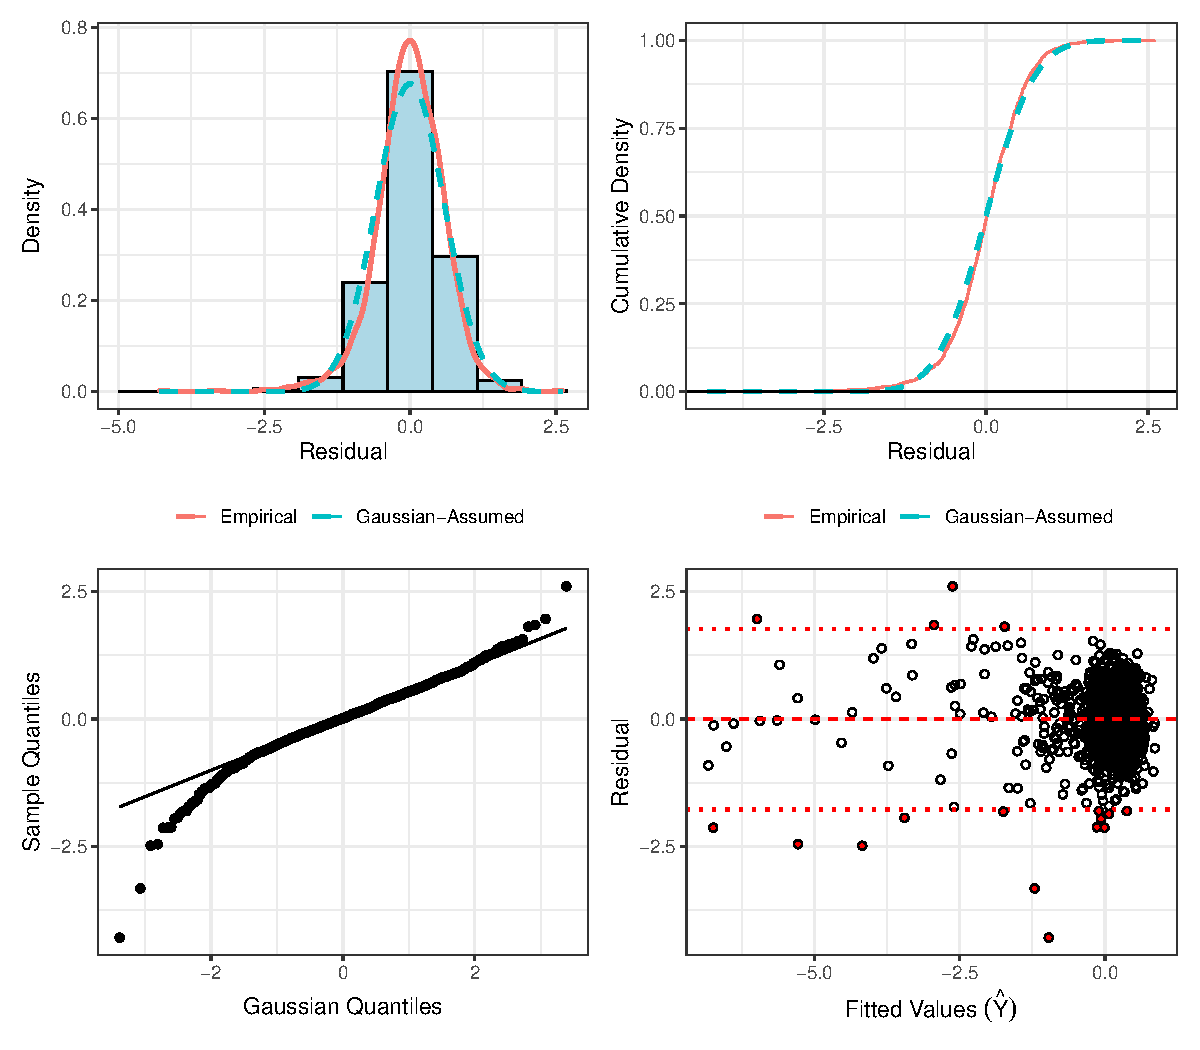
\includegraphics[width=\maxwidth]{figure/unnamed-chunk-34-1} 
\end{knitrout}
\caption{The residuals for our final model.}
\label{step.reduced.accur.residuals}
\end{figure}
\ref{step.reduced.accur.residuals}: A figure of some diagnostic plots for the linear model where Y is birth weights and the predictors are Plural, Sex, MomAgeSC, WeeksSC, Black, GainedSC, Smoke, Premie, Plural:WeeksSC, MomAgeSC:Smoke, WeeksSC:Black, WeeksSC:GainedSC, WeeksSC:Smoke, WeeksSC:Premie, Black:Smoke, and Black:Premie.

As seen in \ref{step.reduced.accur.residuals}, the constant variance assumption is met for the most part and the normality assumption is met. 
\end{enumerate}

\item{\textbf{Influence analysis}}
\begin{enumerate}[i.]
\item Leverage Points \\

From our Exploratory Analysis, we already knew that we had some outline instances. This section will help us determine if any of those outliers are actually significant.

Our function first calculated 191 high leverage values and 100 very high leverage values. They were distributed in the dataset as follows:

\begin{knitrout}
\definecolor{shadecolor}{rgb}{0.969, 0.969, 0.969}\color{fgcolor}\begin{kframe}
\begin{alltt}
  \hlstd{p} \hlkwb{<-} \hlnum{18}
  \hlcom{#leverage points}
  \hlstd{lev} \hlkwb{<-} \hlstd{step.reduced.accur}\hlopt{$}\hlstd{model} \hlopt \hlkwd{mutate}\hlstd{(}\hlkwc{h.values} \hlstd{=} \hlkwd{hatvalues}\hlstd{(step.reduced.accur))}
  \hlcom{#high leverage points }
  \hlstd{n} \hlkwb{<-} \hlkwd{nrow}\hlstd{(step.reduced.accur}\hlopt{$}\hlstd{model)}

  \hlstd{high.lev} \hlkwb{<-} \hlstd{lev} \hlopt \hlkwd{filter}\hlstd{(h.values} \hlopt{>} \hlnum{2}\hlopt{*}\hlstd{p}\hlopt{/}\hlstd{n)}
  \hlcom{#very high leverage points}
  \hlstd{v.high.lev} \hlkwb{<-} \hlstd{lev} \hlopt \hlkwd{filter}\hlstd{(h.values} \hlopt{>} \hlnum{3}\hlopt{*}\hlstd{p}\hlopt{/}\hlstd{n)}

  \hlstd{lev} \hlkwb{<-} \hlstd{lev} \hlopt \hlkwd{mutate}\hlstd{(}\hlkwc{Level} \hlstd{=} \hlkwd{case_when}\hlstd{(h.values} \hlopt{<}\hlnum{2}\hlopt{*}\hlstd{p}\hlopt{/}\hlstd{n} \hlopt{~} \hlstr{"Normal"}\hlstd{,}
                                          \hlstd{h.values} \hlopt{<} \hlnum{3}\hlopt{*}\hlstd{p}\hlopt{/}\hlstd{n} \hlopt{~} \hlstr{"High"}\hlstd{,}
                                          \hlstd{T} \hlopt{~} \hlstr{"Very High"}\hlstd{))}

  \hlstd{lev} \hlopt \hlkwd{ggplot}\hlstd{(}\hlkwd{aes}\hlstd{(}\hlkwc{x}\hlstd{=}\hlkwd{as.numeric}\hlstd{(}\hlkwd{row.names}\hlstd{(.)),} \hlkwc{y}\hlstd{=h.values,} \hlkwc{color}\hlstd{=Level))} \hlopt{+}
    \hlkwd{geom_point}\hlstd{()} \hlopt{+}
    \hlkwd{geom_hline}\hlstd{(}\hlkwc{yintercept}\hlstd{=}\hlnum{3}\hlopt{*}\hlstd{p}\hlopt{/}\hlstd{n,} \hlkwc{linetype}\hlstd{=}\hlstr{"dashed"}\hlstd{,} \hlkwc{color} \hlstd{=} \hlstr{"red"}\hlstd{)} \hlopt{+}
    \hlkwd{geom_hline}\hlstd{(}\hlkwc{yintercept}\hlstd{=}\hlnum{2}\hlopt{*}\hlstd{p}\hlopt{/}\hlstd{n,} \hlkwc{linetype}\hlstd{=}\hlstr{"dashed"}\hlstd{,} \hlkwc{color}\hlstd{=} \hlstr{"blue"}\hlstd{)} \hlopt{+}
    \hlkwd{scale_y_continuous}\hlstd{(}\hlkwc{trans}\hlstd{=}\hlstr{'log2'}\hlstd{)} \hlopt{+}
    \hlkwd{ylab}\hlstd{(}\hlstr{"H-Value (Logarithmic Scale)"}\hlstd{)} \hlopt{+}
    \hlkwd{xlab}\hlstd{(}\hlstr{"Index"}\hlstd{)} \hlopt{+}
    \hlkwd{ggtitle}\hlstd{(}\hlstr{"H-Value Distribution"}\hlstd{)} \hlopt{+}
    \hlkwd{theme_bw}\hlstd{()}
\end{alltt}
\end{kframe}
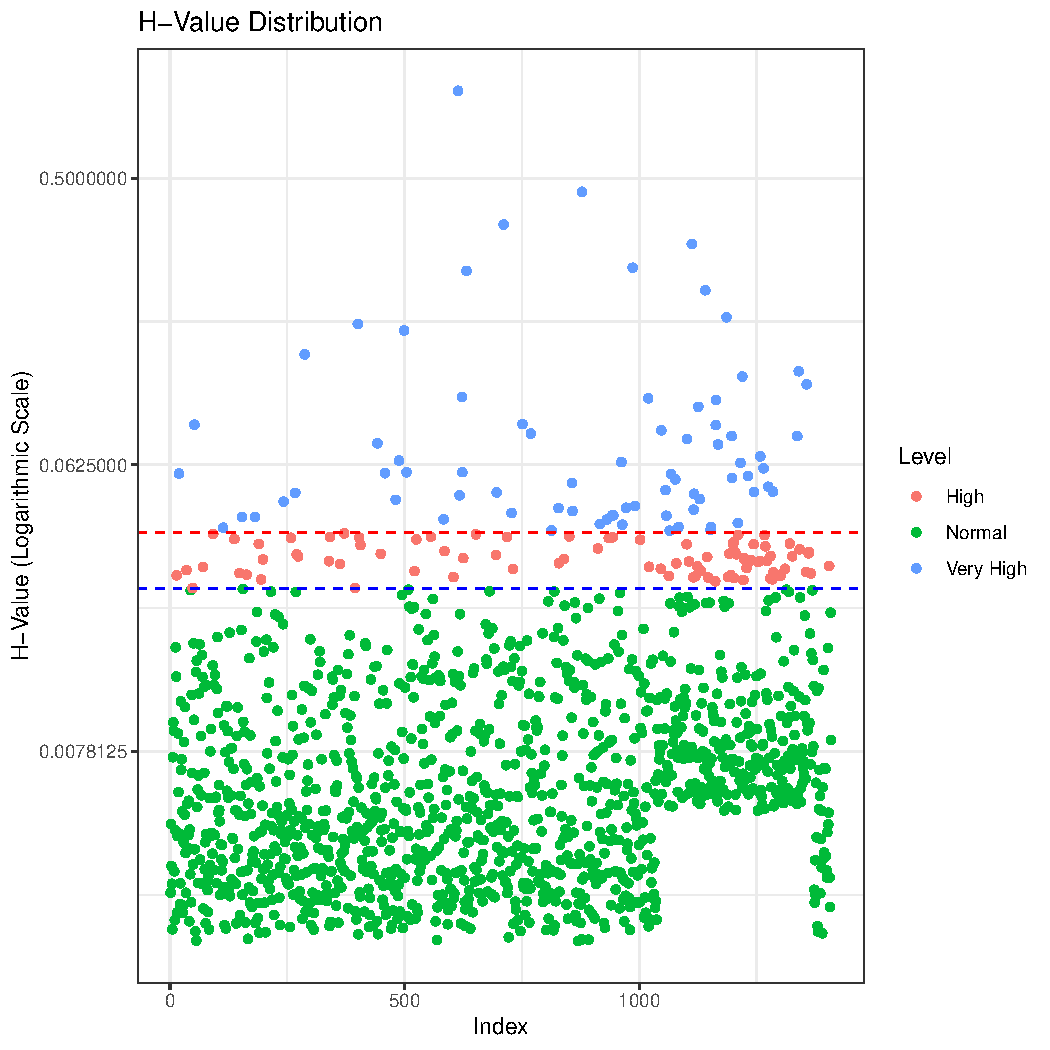
\includegraphics[width=\maxwidth]{figure/unnamed-chunk-35-1} 
\end{knitrout}

\begin{table}[H]
\centering
\begin{tabular}{rrrrrr}
  \hline
   Min. & 1st Qu. &  Median &  Mean  & 3rd Qu. &  Max \\ 
  \hline
  0.001977 & 0.003557 & 0.006024 & 0.013485 & 0.012288 & 0.942679 \\
   \hline
\end{tabular}
\label{High Leverage Values Quantile Summary}
\caption{High Leverage Values Quantile Summary.}
\end{table}


\item Standardized/Studentized Residuals\\
Next, our function output the summaries of the Standardized/Studentized Residuals and the outliers of our dataset. \\

\begin{table}[H]
\centering
\begin{tabular}{rrrrrr}
  \hline
   Min. & 1st Qu. &  Median &  Mean  & 3rd Qu. &  Max \\ 
  \hline
  -7.313842 & -0.546892 & 0.022207 & -0.000838 & 0.642574 & 4.483741 \\
   \hline
\end{tabular}
\label{Standardized Residuals Quantile Summary}
\caption{Standardized Residuals Quantile Summary.}
\end{table}

\begin{knitrout}
\definecolor{shadecolor}{rgb}{0.969, 0.969, 0.969}\color{fgcolor}\begin{kframe}
\begin{alltt}
    \hlstd{new.resid} \hlkwb{<-} \hlstd{step.reduced.accur}\hlopt{$}\hlstd{model} \hlopt \hlkwd{mutate}\hlstd{(}\hlkwc{stdres} \hlstd{=} \hlkwd{rstandard}\hlstd{(step.reduced.accur),}
                                      \hlkwc{stures} \hlstd{=} \hlkwd{rstudent}\hlstd{(step.reduced.accur))}

    \hlcom{#outliers}
  \hlstd{s.outliers.stdres} \hlkwb{<-} \hlstd{new.resid} \hlopt \hlkwd{mutate}\hlstd{(}\hlkwc{stdres_level} \hlstd{=} \hlkwd{case_when} \hlstd{(}\hlkwd{abs}\hlstd{(stdres)}\hlopt{>}\hlnum{3} \hlopt{~} \hlstr{"High"}\hlstd{, T} \hlopt{~} \hlstr{"Low"}\hlstd{))}
  \hlstd{s.outliers.stures} \hlkwb{<-} \hlstd{new.resid} \hlopt \hlkwd{mutate}\hlstd{(}\hlkwc{stures_level} \hlstd{=} \hlkwd{case_when} \hlstd{(}\hlkwd{abs}\hlstd{(stures)}\hlopt{>}\hlnum{3} \hlopt{~} \hlstr{"High"}\hlstd{, T} \hlopt{~} \hlstr{"Low"}\hlstd{))}

  \hlstd{s.outliers.stdres} \hlopt \hlkwd{ggplot}\hlstd{(}\hlkwd{aes}\hlstd{(}\hlkwc{x}\hlstd{=}\hlkwd{as.numeric}\hlstd{(}\hlkwd{row.names}\hlstd{(.)),} \hlkwc{y}\hlstd{=stdres,} \hlkwc{color}\hlstd{=stdres_level))} \hlopt{+}
    \hlkwd{geom_point}\hlstd{()} \hlopt{+}
    \hlkwd{geom_hline}\hlstd{(}\hlkwc{yintercept}\hlstd{=}\hlnum{3}\hlstd{,} \hlkwc{linetype}\hlstd{=}\hlstr{"dashed"}\hlstd{,} \hlkwc{color} \hlstd{=} \hlstr{"red"}\hlstd{)} \hlopt{+}
    \hlkwd{geom_hline}\hlstd{(}\hlkwc{yintercept}\hlstd{=}\hlopt{-}\hlnum{3}\hlstd{,} \hlkwc{linetype}\hlstd{=}\hlstr{"dashed"}\hlstd{,} \hlkwc{color}\hlstd{=} \hlstr{"blue"}\hlstd{)} \hlopt{+}
    \hlkwd{ylab}\hlstd{(}\hlstr{"Standardized Residuals"}\hlstd{)} \hlopt{+}
    \hlkwd{xlab}\hlstd{(}\hlstr{"Index"}\hlstd{)} \hlopt{+}
    \hlkwd{ggtitle}\hlstd{(}\hlstr{"Standardized Residual Distribution"}\hlstd{)} \hlopt{+}
    \hlkwd{theme_bw}\hlstd{()}  \hlkwb{->} \hlstd{stdres_plot}

  \hlstd{s.outliers.stures} \hlopt \hlkwd{ggplot}\hlstd{(}\hlkwd{aes}\hlstd{(}\hlkwc{x}\hlstd{=}\hlkwd{as.numeric}\hlstd{(}\hlkwd{row.names}\hlstd{(.)),} \hlkwc{y}\hlstd{=stures,} \hlkwc{color}\hlstd{=stures_level))} \hlopt{+}
    \hlkwd{geom_point}\hlstd{()} \hlopt{+}
    \hlkwd{geom_hline}\hlstd{(}\hlkwc{yintercept}\hlstd{=}\hlnum{3}\hlstd{,} \hlkwc{linetype}\hlstd{=}\hlstr{"dashed"}\hlstd{,} \hlkwc{color} \hlstd{=} \hlstr{"red"}\hlstd{)} \hlopt{+}
    \hlkwd{geom_hline}\hlstd{(}\hlkwc{yintercept}\hlstd{=}\hlopt{-}\hlnum{3}\hlstd{,} \hlkwc{linetype}\hlstd{=}\hlstr{"dashed"}\hlstd{,} \hlkwc{color}\hlstd{=} \hlstr{"blue"}\hlstd{)} \hlopt{+}
    \hlkwd{ylab}\hlstd{(}\hlstr{"Studentized Residuals"}\hlstd{)} \hlopt{+}
    \hlkwd{xlab}\hlstd{(}\hlstr{"Index"}\hlstd{)} \hlopt{+}
    \hlkwd{ggtitle}\hlstd{(}\hlstr{"Studentized Residual Distribution"}\hlstd{)} \hlopt{+}
    \hlkwd{theme_bw}\hlstd{()}  \hlkwb{->} \hlstd{stures_plot}

  \hlstd{stdres_plot} \hlopt{+} \hlstd{stures_plot}
\end{alltt}
\end{kframe}
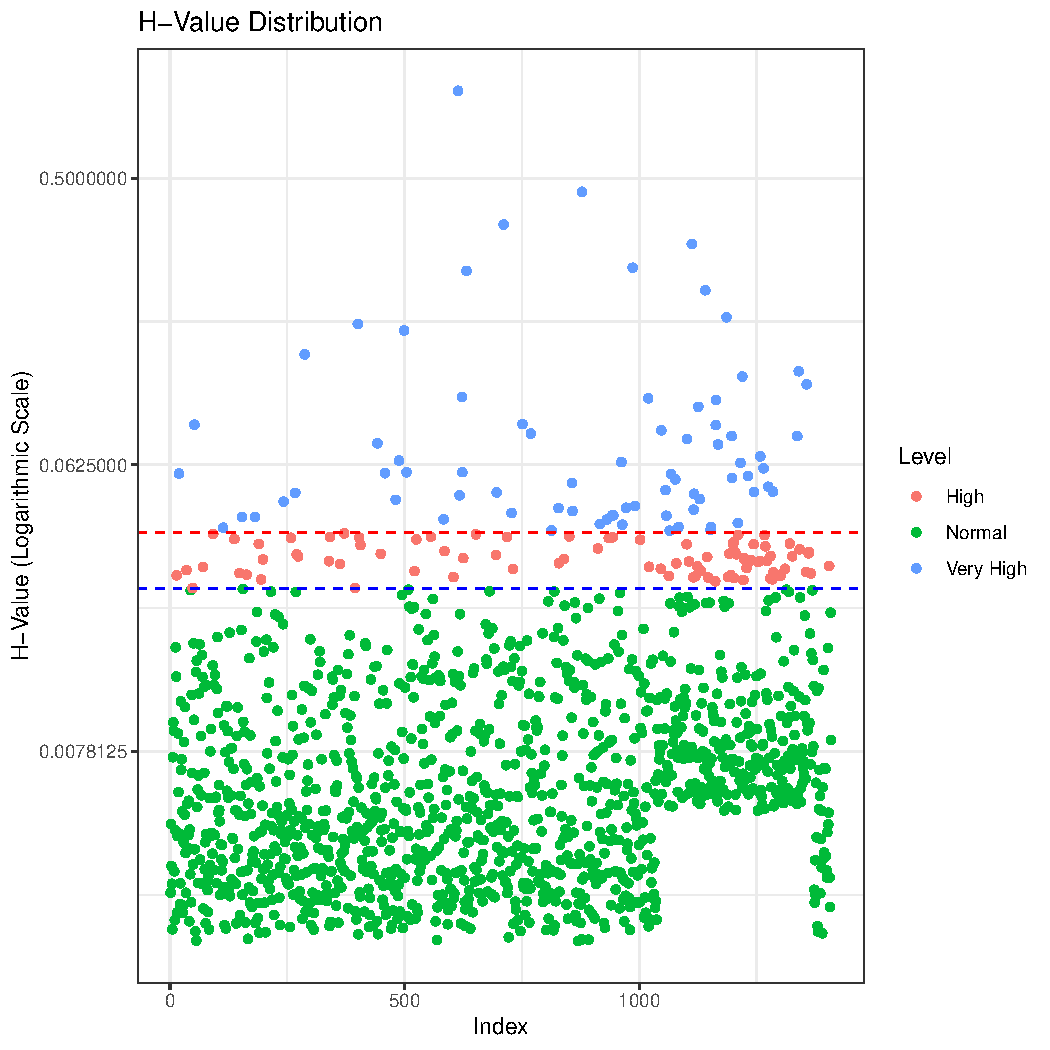
\includegraphics[width=\maxwidth]{figure/unnamed-chunk-36-1} 
\end{knitrout}


\begin{table}[H]
\centering
\begin{tabular}{rrrrrr}
  \hline
   Min. & 1st Qu. &  Median &  Mean  & 3rd Qu. &  Max \\ 
  \hline
  -7.456087 & -0.546754 & 0.022199 & -0.001093 &  0.642438 & 4.514897 \\
   \hline
\end{tabular}
\label{Studentized Residuals Quantile Summary}
\caption{Studentized Residuals Quantile Summary.}
\end{table}

\item Outliers\\

From our previous calculation of the high leverage values, we found 17 outlier instances in our dataset that fell outside the expected departures from our residual curve. They are listed in the table below:

\begin{table}[H]
\centering
\begin{tabular}{rrrrrrrrr}
  \hline
   WeightLog (SC) & Plural & Sex & MomAge (SC) & Weeks (SC) Black & Gained (SC) & Smoke & Premie \\ 
  \hline
  -1.79825625 & 1 & Male & -0.94445468 & -0.2301192 & FALSE & -0.7639289 & No & No\\
  -2.02393397 & 1 &  Male & -0.94445468 & 0.5108647 & FALSE & -1.0521654 & Yes &  No \\
  -2.14180198 & 1 & Female & -0.94445468 & 0.5108647 & FALSE & -1.8448158 & No & No \\
  -1.90948290 & 1 & Female & -0.28842628  & 1.6223405 & FALSE & -0.9080472 & Yes & No \\ 
  -1.09672028 & 1 &  Male & -1.27246888 & -2.8235628 &  FALSE & -1.4845202 & No & Yes\\
  -5.38870953 & 1 & Male & -0.94445468 & -3.5645467 & FALSE  & 0.1728397 & No & Yes\\
  -3.56718564 & 1 &  Male & 0.03958792 & -2.4530708 & FALSE & 1.0375492 & No & Yes\\
  -4.53499902 & 1 & Male & 0.20359502 & -1.7120870 & FALSE & -0.7639289 & Yes & Yes\\
  -6.66311095 & 1 & Male & -0.78044758 & -3.9350386 & FALSE & -0.7639289 & No & Yes\\
  -5.25485653 & 1 & Female & -1.43647598 & -1.3415950 & FALSE & -0.8359881 & No & Yes\\
  -7.73678282 & 1 & Male & -1.27246888 &-4.3055305 & TRUE & -1.4124611  & No & Yes\\
  -8.87263370 & 2 & Female & -1.10846178 & -6.1579902 & TRUE & 0.6772536 & No & Yes\\
  -2.26329727 & 1 & Male & -0.45243338 & -0.6006112 & TRUE & 0.1728397 & No & No\\
  -4.02151218 & 1 & Female & -1.43647598 & -4.6760225 & TRUE & -1.4845202 & No & Yes\\
   0.08477603 & 1 & Female & 0.53160922 & -2.4530708 & TRUE & 0.8934309 & Yes & Yes\\
  -0.01867841 & 1 & Male & 0.69561632 & -2.8235628 & TRUE & -0.3315742 & No & Yes\\
  -1.43192750 & 1 & Male & -0.45243338 & 0.1403727 & FALSE & 0.8213718 & No & No\\
   \hline
\end{tabular}
\label{}
\caption{Outliers that are outside the expected departure.}
\end{table}


\item Influential Observations\\
\begin{table}[H]
\centering
\begin{tabular}{rrrrrr}
  \hline
   Min. & 1st Qu. &  Median &  Mean  & 3rd Qu. &  Max \\ 
  \hline
  0.0000000 & 0.0000240 & 0.0001095 & 0.0014421 & 0.0004313 & 0.4464716 \\
   \hline
\end{tabular}
\label{Cook's test Quantile Summary}
\caption{Cook's test Quantile Summary.}
\end{table}
\end{enumerate}

After calculating Cook's distane, we found that there were no instances with values greater than 1, and thus no influential observations in the dataset. 

\begin{knitrout}
\definecolor{shadecolor}{rgb}{0.969, 0.969, 0.969}\color{fgcolor}\begin{kframe}
\begin{alltt}
  \hlstd{cooks.values} \hlkwb{<-} \hlstd{step.reduced.accur}\hlopt{$}\hlstd{model} \hlopt \hlkwd{mutate}\hlstd{(}\hlkwc{Cooks} \hlstd{=} \hlkwd{cooks.distance}\hlstd{(step.reduced.accur))}
  \hlstd{cooks.values} \hlopt \hlkwd{ggplot}\hlstd{(}\hlkwd{aes}\hlstd{(}\hlkwc{x}\hlstd{=}\hlkwd{as.numeric}\hlstd{(}\hlkwd{row.names}\hlstd{(.)),} \hlkwc{y}\hlstd{=Cooks))} \hlopt{+}
    \hlkwd{geom_point}\hlstd{()} \hlopt{+}
    \hlkwd{geom_hline}\hlstd{(}\hlkwc{yintercept}\hlstd{=}\hlnum{1}\hlstd{,} \hlkwc{linetype}\hlstd{=}\hlstr{"dashed"}\hlstd{,} \hlkwc{color} \hlstd{=} \hlstr{"red"}\hlstd{)} \hlopt{+}
    \hlkwd{ylab}\hlstd{(}\hlstr{"Cook's Distance (Square Root Scale)"}\hlstd{)} \hlopt{+}
    \hlkwd{xlab}\hlstd{(}\hlstr{"Index"}\hlstd{)} \hlopt{+}
    \hlkwd{ggtitle}\hlstd{(}\hlstr{"Cook's Distance Distribution"}\hlstd{)} \hlopt{+}
        \hlkwd{scale_y_continuous}\hlstd{(}\hlkwc{trans}\hlstd{=}\hlstr{'sqrt'}\hlstd{)} \hlopt{+}
    \hlkwd{theme_bw}\hlstd{()}  \hlkwb{->} \hlstd{cooks_plot}

  \hlstd{cooks_plot}
\end{alltt}
\end{kframe}
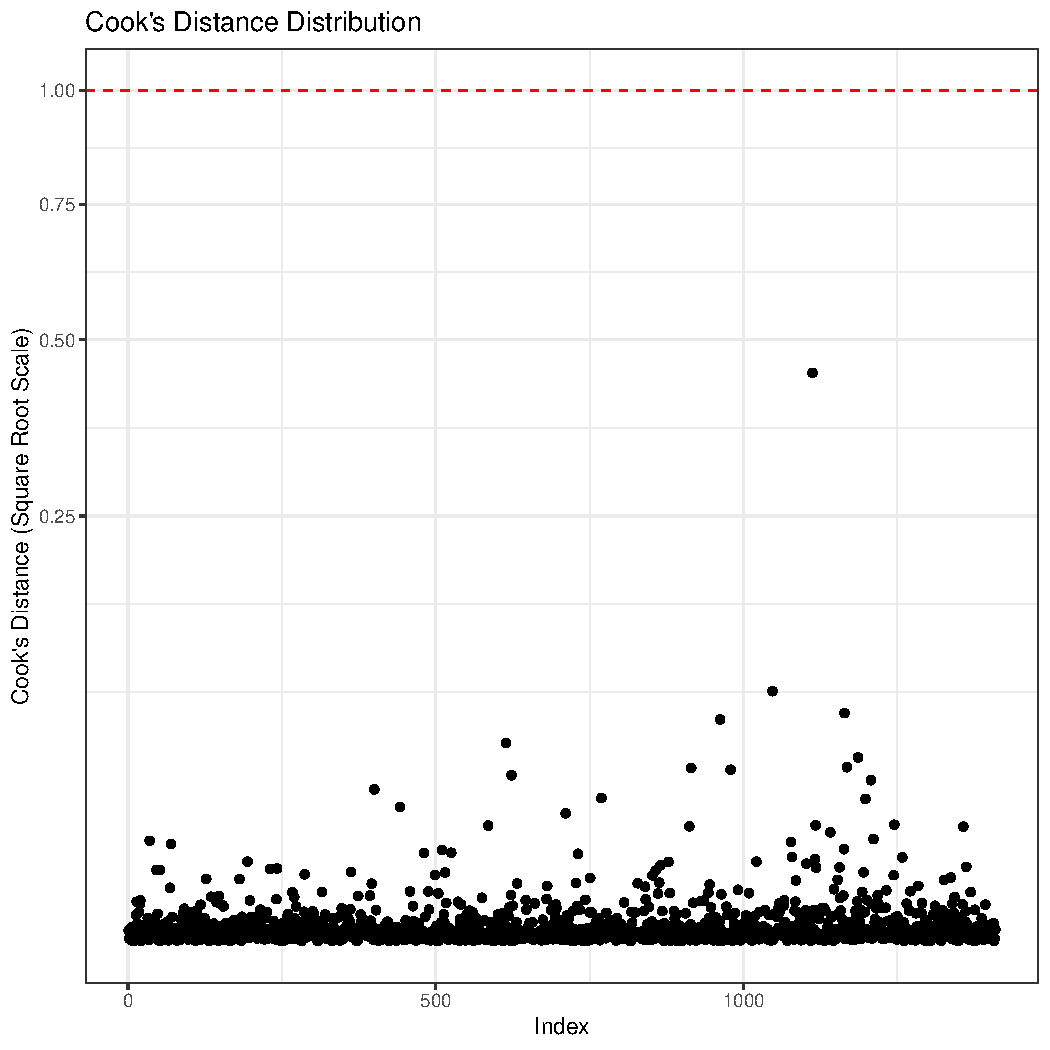
\includegraphics[width=\maxwidth]{figure/unnamed-chunk-37-1} 
\end{knitrout}

\item{\textbf{Summarize the findings of your final models}}
\begin{enumerate}[i.]
\item Fitted Model
\begin{knitrout}
\definecolor{shadecolor}{rgb}{0.969, 0.969, 0.969}\color{fgcolor}\begin{kframe}
\begin{alltt}
\hlkwd{xtable}\hlstd{(}\hlkwd{round}\hlstd{(}\hlkwd{summary}\hlstd{(step.reduced.accur)}\hlopt{$}\hlstd{coefficients,}\hlnum{4}\hlstd{))}
\end{alltt}
\end{kframe}
\end{knitrout}


\begin{table}[H]
\centering
\begin{tabular}{rrrrr}
  \hline
 & Estimate & Std. Error & t value & Pr($>$$|$t$|$) \\ 
  \hline
(Intercept) & 0.18 & 0.03 & 6.49 & 0.00 \\ 
  Twin & -1.23 & 0.14 & -8.97 & 0.00 \\ 
  Triplet & -1.03 & 0.63 & -1.64 & 0.10 \\ 
  Male & 0.11 & 0.03 & 3.51 & 0.00 \\ 
  MomAge (SC) & 0.09 & 0.02 & 5.14 & 0.00 \\ 
  Weeks (SC) & 0.17 & 0.03 & 5.26 & 0.00 \\ 
  Black & -0.22 & 0.05 & -4.66 & 0.00 \\ 
  Gained (SC) & 0.12 & 0.02 & 7.80 & 0.00 \\ 
  SmokeYes & -0.27 & 0.05 & -5.22 & 0.00 \\ 
  PremieYes & 0.85 & 0.10 & 8.10 & 0.00 \\ 
  Twin:Weeks (SC) & -0.30 & 0.07 & -4.25 & 0.00 \\ 
  Triplet:Weeks (SC) & -0.10 & 0.21 & -0.46 & 0.65 \\ 
  MomAgeSC:SmokeYes & -0.10 & 0.05 & -2.16 & 0.03 \\ 
  WeeksSC:Black & 0.16 & 0.05 & 3.05 & 0.00 \\ 
  WeeksSC:Gained (SC) & -0.04 & 0.02 & -2.50 & 0.01 \\ 
  WeeksSC:SmokeYes & -0.15 & 0.04 & -3.56 & 0.00 \\ 
  WeeksSC:PremieYes & 1.11 & 0.06 & 18.45 & 0.00 \\ 
  Black:SmokeYes & 0.16 & 0.11 & 1.42 & 0.16 \\ 
  Black:PremieYes & 0.53 & 0.15 & 3.44 & 0.00 \\ 
   \hline
\end{tabular}
\end{table}

\item Confidence intervals for partial slope parameters
\begin{knitrout}
\definecolor{shadecolor}{rgb}{0.969, 0.969, 0.969}\color{fgcolor}\begin{kframe}
\begin{alltt}
\hlkwd{xtable}\hlstd{(confint2000}\hlkwb{<-}\hlkwd{confint}\hlstd{(model.3.assu,} \hlkwc{level}\hlstd{=}\hlnum{0.95}\hlstd{))}
\end{alltt}
\end{kframe}
\end{knitrout}
\begin{table}[H]
\centering
\begin{tabular}{rrr}
  \hline
 & 2.5 \% & 97.5 \% \\ 
  \hline
(Intercept) & 0.03 & 0.16 \\ 
  Twin & -1.36 & -0.88 \\ 
  Triplet & -2.21 & -0.73 \\ 
  Male & 0.07 & 0.23 \\ 
  MomAge (SC) & 0.08 & 0.16 \\ 
  Weeks (SC) & 0.36 & 0.48 \\ 
  Black & -0.29 & -0.10 \\ 
  Gained (SC) & 0.13 & 0.21 \\ 
  SmokeYes & -0.45 & -0.22 \\ 
  PremieYes & -0.52 & -0.19 \\ 
   \hline
\end{tabular}
\end{table}

\end{enumerate}

\end{enumerate}

Highest Accuracy Model: -> mod.accur.prelim.full 
\begin{align*}
\hat{y} &= 0.1813 - 1.2273\cdot \text{I}(\text{Twin} = \text{TRUE}) - 1.0309\cdot \text{I}(\text{Triplet} = \text{TRUE}) + 0.1110\cdot \text{I}(\text{Sex} = \text{Male}) + 0.0912\cdot \text{MomAgeSC} \\
&\quad + 0.1688\cdot \text{WeeksSC} - 0.2197\cdot \text{I}(\text{Black} = \text{TRUE}) + 0.1250\cdot \text{GainedSC} - 0.2696\cdot \text{I}(\text{Smoke} = \text{Yes}) + 0.8473\cdot \text{I}(\text{Preemie} = \text{Yes}) \\
&\quad - 0.2970\cdot \text{I}(\text{Twin} = \text{TRUE})\cdot \text{WeeksSC} - 0.0969\cdot \text{I}(\text{Triplet} = \text{TRUE})\cdot \text{WeeksSC} - 0.1005\cdot \text{MomAgeSC}\cdot \text{I}(\text{Smoke} = \text{Yes}) \\ &\quad + 0.1588\cdot \text{WeeksSC}\cdot \text{I}(\text{Black} = \text{TRUE}) - 0.0422\cdot \text{WeeksSC}\cdot \text{GainedSC} - 0.1502\cdot \text{WeeksSC}\cdot \text{I}(\text{Smoke} = \text{Yes}) + 1.1080\cdot \text{WeeksSC}\cdot \text{I}(\text{Preemie} = \text{Yes}) \\
&\quad + 0.1590\cdot \text{I}(\text{Black} = \text{TRUE})\cdot \text{I}(\text{Smoke} = \text{Yes}) + 0.5283\cdot \text{I}(\text{Black} = \text{TRUE})\cdot \text{I}(\text{Preemie} = \text{Yes})
\end{align*}

Non-Interact Assumptions Model -> model.3.assu
\begin{align*}
\hat{y} &= 0.0948 - 1.1201\cdot \text{I}(\text{Twin} = \text{TRUE}) - 1.4721\cdot \text{I}(\text{Triplet} = \text{TRUE}) + 0.1522\cdot \text{I}(\text{Sex} = \text{Male}) \\
&\quad + 0.1186\cdot \text{MomAgeSC} + 0.4187\cdot \text{WeeksSC} - 0.1917\cdot \text{I}(\text{Black} = \text{TRUE}) + 0.1738\cdot \text{GainedSC} \\
&\quad - 0.3343\cdot \text{I}(\text{Smoke} = \text{Yes}) - 0.3577\cdot \text{I}(\text{Preemie} = \text{Yes})
\end{align*}

\bibliography{bibliography.bib}

\end{document}
